\documentclass[twoside,10pt,a4paper, openright, hidelinks]{extreport}
\usepackage[english]{babel}
\usepackage[T1]{fontenc}
\usepackage{kpfonts}
\usepackage[utf8]{inputenc}
\usepackage{float}
\usepackage[parfill]{parskip}
\usepackage{listings}
\usepackage{setspace}
\usepackage{multicol}
%%\usepackage{calc}
\usepackage{enumerate}
\usepackage{amsmath}
\usepackage{amssymb}
\usepackage{url}
\usepackage{hyperref}
\usepackage{cleveref}
\usepackage{graphicx}
%\usepackage{caption}
\usepackage{subcaption}
\usepackage{natbib}
\usepackage{minitoc}
\usepackage{bibentry}
\usepackage[Lenny]{fncychap}
\usepackage{cases}
\usepackage{fancybox}
%%\usepackage{subfig}
\usepackage{supertabular}
\usepackage{multirow}
\usepackage{blindtext}
%%\usepackage{newtxtext,newtxmath}
\usepackage{rotating}
\usepackage{lscape}
\usepackage{wrapfig}
\usepackage[font={small}]{caption}
\usepackage{array}

% FONT %
%\usepackage[sfdefault]{quattrocento}
%\usepackage[T1]{fontenc}

\usepackage[default,oldstyle,scale=0.95]{opensans} %% Alternatively
%% use the option 'defaultsans' instead of 'default' to replace the
%% sans serif font only.
\usepackage[T1]{fontenc}

\usepackage{wrapfig}

%%%% PAGE DIMENSIONS

%\usepackage[a5paper]{meta-donnees}
%\newcommand{\new}[1]{\textcolor{red}{#1}}
\usepackage[final]{pdfpages}
%\usepackage{meta-donnees}
\usepackage{xspace} 
\usepackage{etoolbox}  % or xpatch
\usepackage{booktabs}
\usepackage[normalem]{ulem}
\useunder{\uline}{\ul}{}
\usepackage{lineno}
\usepackage{placeins}

\usepackage{fancyhdr} %for nice page headers
\fancyhf{}
\fancyfoot{}
\fancyhead[LE,RO]{\small{\thepage}}
\fancyhead[LO]{\nouppercase{\leftmark}}
\fancyhead[RE]{}

%\usepackage[top=1.5cm,bottom=1.5cm,left=1.5cm,right=1.5cm]{geometry}
%\usepackage[papersize={170mm,240mm},top=1.5cm,bottom=1.5cm,left=1.5cm,right=1.5cm]{geometry}
\usepackage{geometry}
\geometry{a4paper} 
\geometry{margin=2.7cm}
\usepackage{pdfpages}

\setlength{\parindent}{0.5cm} % Default is 15pt.
\setlength{\parskip}{0.1 cm}

\usepackage{setspace}

%\linenumbers


%% edit by Fanny: definition of the encart environnment and associated counter
\newcounter{encartcompteur}[chapter]
\renewcommand{\theencartcompteur}{\arabic{chapter}.\arabic{encartcompteur}}

\newcommand{\encart}[2]{
\refstepcounter{encartcompteur}
\label{box:#1}
%\setlabel{#1}
\begin{wrapfigure}{r}{9cm}
\boxput*(0,1){\colorbox{white}{\textbf{Box \arabic{chapter}.\arabic{encartcompteur}: #1}}}{
\setlength
{\fboxsep}{14pt}
\fbox
{\begin{minipage}{8cm}
#2
\end{minipage}}
}
\end{wrapfigure}
}

\newcommand{\encartl}[2]{
\refstepcounter{encartcompteur}
\label{box:#1}
%\setlabel{#1}
\begin{wrapfigure}{l}{9cm}
\boxput*(0,1){\colorbox{white}{\textbf{Box \arabic{chapter}.\arabic{encartcompteur}: #1}}}{
\setlength
{\fboxsep}{14pt}
\fbox
{\begin{minipage}{7cm}
#2
\end{minipage}}
}
\end{wrapfigure}
}


\newcommand{\mwe}{m w.e. a$^{-1}$\xspace}

%\singlespacing
\onehalfspacing
%\doublespacing
%\setstretch{1.1}

%\linespread{1.2}
%\linespread{1.5}


\begin{document}

%\includepdf[pages=-]{D:/01_these/manuscrit/latex_files/couverture/couverture_these.pdf}
\newpage\null\thispagestyle{empty}\setcounter{page}{0}\newpage

\pagestyle{fancy}

\nobibliography*
\pagenumbering{roman}
\dominitoc


%\newpage\null\thispagestyle{empty}\newpage
\vspace*{\stretch{1}}
\begin{flushright}
\begin{small}
\textit{To my parents.}
\end{small}
\end{flushright}
\vspace*{\stretch{2}}
\newpage\null\thispagestyle{empty}\newpage


\section*{Abstract}
Fire in the hole
\newpage
%\input{abstract/resume}
%\newpage\null\thispagestyle{empty}\newpage
%\newpage
\section*{Acknowledgements}

This PhD work has been, by all means, a collective effort. I would have never been able to accomplish this without the help, kind words or time from a multitude of people. I am extremely grateful for that, for this work has been an incredible human experience. There are a lot of people that I would like to thank, and I sincerely hope I hope I will not forget anyone. First of all, I would like to thank my parents, for giving me the opportunity and freedom to pursue my studies, which gave me the independence to control my professional career and aim it towards the things I love and matter to me. All of this would not have been possible without Kadia, my closest companion, the hidden co-author, who took care of me during these years despite the long rants on glaciers, climate and machine learning. I am also extremely grateful for the family I have. Laia, Mariona, Andrew, for all the time shared together, especially in New Zealand; and my grandparents, who started showing interest on glaciers in the last years.

Then, I would like to thank my supervisors, who gave me the possibility to do this work, and who always respected my vision and way of working. Antoine, for his availability, dedicating whatever time needed to my problems, and protecting me from several ordeals regarding French paperwork. Being able to discuss in Spanish at the beginning of the PhD was a great way to engage in deep discussions on glaciers, and improved my confidence as a total newcomer to the field. Isabelle, who guided me in the most kind way, and provided invaluable insights on climatology and hydrology. I particularly appreciate the freedom I was given to work on the ideas that drive me, knowing the cost that this represented on her research part. For that, I am grateful, but also sorry for not having managed to include them in a better way. Eric and Thomas, who provided insightful comments throughout my work, and whose hydrological expertise helped me during the last part of this work. 

My PhD companions have proved to be my best allies for such a long journey, with many people I would like to thank. Julien, Joseph, Gabi and Nathan shared with me some of the most memorable adventures on two wheels, from the Alps to Utah. Maria, Gabi, both Juliens, Jai, Jonathan, Joseph and Ambroise shared many hours of skinning up and skiing down snowy mountains, reminding us why we love them so much. Ugo, for the long discussions in the office, attempting to solve the world's problems besides finishing our PhDs, and for the amazing time in Stiappa. Lucas, Olivier and Juan Pedro, for being excellent office partners, and for the stimulating conversations. Romain, Marion, Astrid, Diego, Hans, Foteini, Albane, Sammy, Jinwha, Laura, Pedro, Peter, Sarah, Claudio, Maxim, Fanny and Marco, for the great times shared in the lab, in conferences, in the mountains or at the bar. 

I am also grateful to Delphine, Olivier and Bruno, who taught me how to measure glacier mass balance in the field, in some of the most breathtaking landscapes I have ever seen. I had so much fun doing that, but I will particularly remember the day when, together with Delphine, we measured all the ablation stakes in Mer de Glace in one long and arduous push. I am especially thankful to the members of my PhD jury for accepting to review this work. I have been lucky enough to have exactly the jury I wished for, and I really appreciate the time and effort that it involves. Moreover, I would also like to thank Christian, Thomas and Agnès, for taking part in my thesis committee, and guiding me with insightful comments  and making it feel more like a conversation than an evaluation. There are many people in the lab(s) that I would also like to thank, for the friendly and interesting conversations in the cafeteria and for the shared small talk: Jérémie, Nico, Sophie, Patrick, Jean-Manu, Gilles, Martin, Lionel and Vincent. 

Finally, I am grateful for many scientific interactions I had outside the lab, particularly during conferences and paper reviews. I would like to thank Fabien Maussion, Ben Marzeion and Matthias Huss, who besides being an inspiration for me, they provided constructive feedback that truly managed to improve my work. I can only hope to have the same luck with reviewers in the future. I am also very thankful to Daniel Farinotti, who always showed kind interest in my work from the beginning, and who is currently helping me to pursue my scientific ideas for a postdoc. I had the chance to meet Fernando Pérez in San Francisco last year, resulting in stimulating discussions regarding scientific modelling. I hope we will be able to collaborate in the future, once the currently troubled times calm down.

\bigskip
\bigskip
\bigskip
\bigskip

\begin{flushright}
\begin{small}
\textit{This manuscript has been written and assembled in the beautiful small village of Stiappa, Tuscany (Italy).}
\end{small}
\end{flushright}

\tableofcontents
%\newpage\null\thispagestyle{empty}\newpage

\pagenumbering{arabic}

\chapter{Introduction}
\label{chap:intro}

\begin{flushright}
\begin{small}
\textit{Even in science, the object of research is no longer nature itself, but man's investigation of nature.}\\
Werner Heisenberg
\end{small}
\end{flushright}

\section{On the importance of glaciers}

Glaciers are fascinating natural systems to study. Their beauty originates from complex interactions between climate and topography, creating  unique natural features that shape landscapes, ecosystems and even climates wherever they flow. These perennial ice masses originate in places allowing the accumulation of snow, that over the course of years gradually transform into firn and eventually ice. Due to gravity, this ice flows downwards, reaching lower elevations with higher temperatures where ice is lost through different processes of ablation, such as ice melting or calving \citep{ipcc_climate_2018}. The sum of all accumulation and ablation in a glacier determines its mass balance, which is essential to track the evolution of glaciers through time and their contribution to sea level rise (Fig. \ref{intro:fig1}). Glaciers are excellent climate proxies, adjusting their geometry and size to changes in climate. They represent a large part of the cryosphere, covering some 10\% of the Earth's land surface and storing about 69\% of the world's fresh water \citep{cuffey_physics_2010}. In their study, glaciers are often divided into mountain glaciers (Fig. \ref{intro:fig1}) and ice-sheets, which differ in size and geographical location, with ice-sheets being much larger than mountain glaciers and situated in Greenland and Antarctica \citep{benn_glaciers_2014}.  

Mountains are the water towers of the world, acting as buffers that store solid precipitation and distribute fresh water resources throughout the year \citep{immerzeel_importance_2020}. Seasonal and long-term cryospheric changes in mountain environments regulate water, nutrient and sediment supply downstream \citep{huss_toward_2017}. Glaciers play a major role in this, providing water resources during the warmest months well after all snow has melted. This late summer runoff is essential to many ecosystems requiring cold water and humid habitats throughout the year \citep{cauvy-fraunie_global_2019, carlson_monitoring_2020}. About 10\% of the global population live in mountain areas and the contiguous plains, depending on these water resources for agriculture, industry, hydropower or domestic use \citep{huss_global-scale_2018,farinotti_large_2019}.  Mountain areas are amongst the most affected regions by anthropogenic climate change, outpacing global warming  with an increase of 0.3ºC per decade \citep{ipcc_climate_2018}. These rapid changes in climate are causing a widespread retreat of glaciers (Fig. \ref{intro:fig1}), with many regions already having reached "peak water", i.e. the maximum annual glacier runoff. Once this point is reached, glaciers progressively reduce their water contributions, altering the hydrological regime of watersheds \citep{huss_global-scale_2018}. The disappearance of glaciers produces an early release of accumulated precipitation in spring and early summer, with potential droughts in late summer \citep{brunner_future_2019}. These fast changes in mountain glaciers result in glaciers currently being important contributors to sea level rise (0.92 $\pm$ 0.39 mm a$^{-1}$), as much as the massive Antarctic and Greenland ice-sheets combined, despite representing less than 1\% of the ice on Earth \citep{zemp_global_2019, hock_glaciermip_2019}. 

\begin{figure*}[h]
\centering
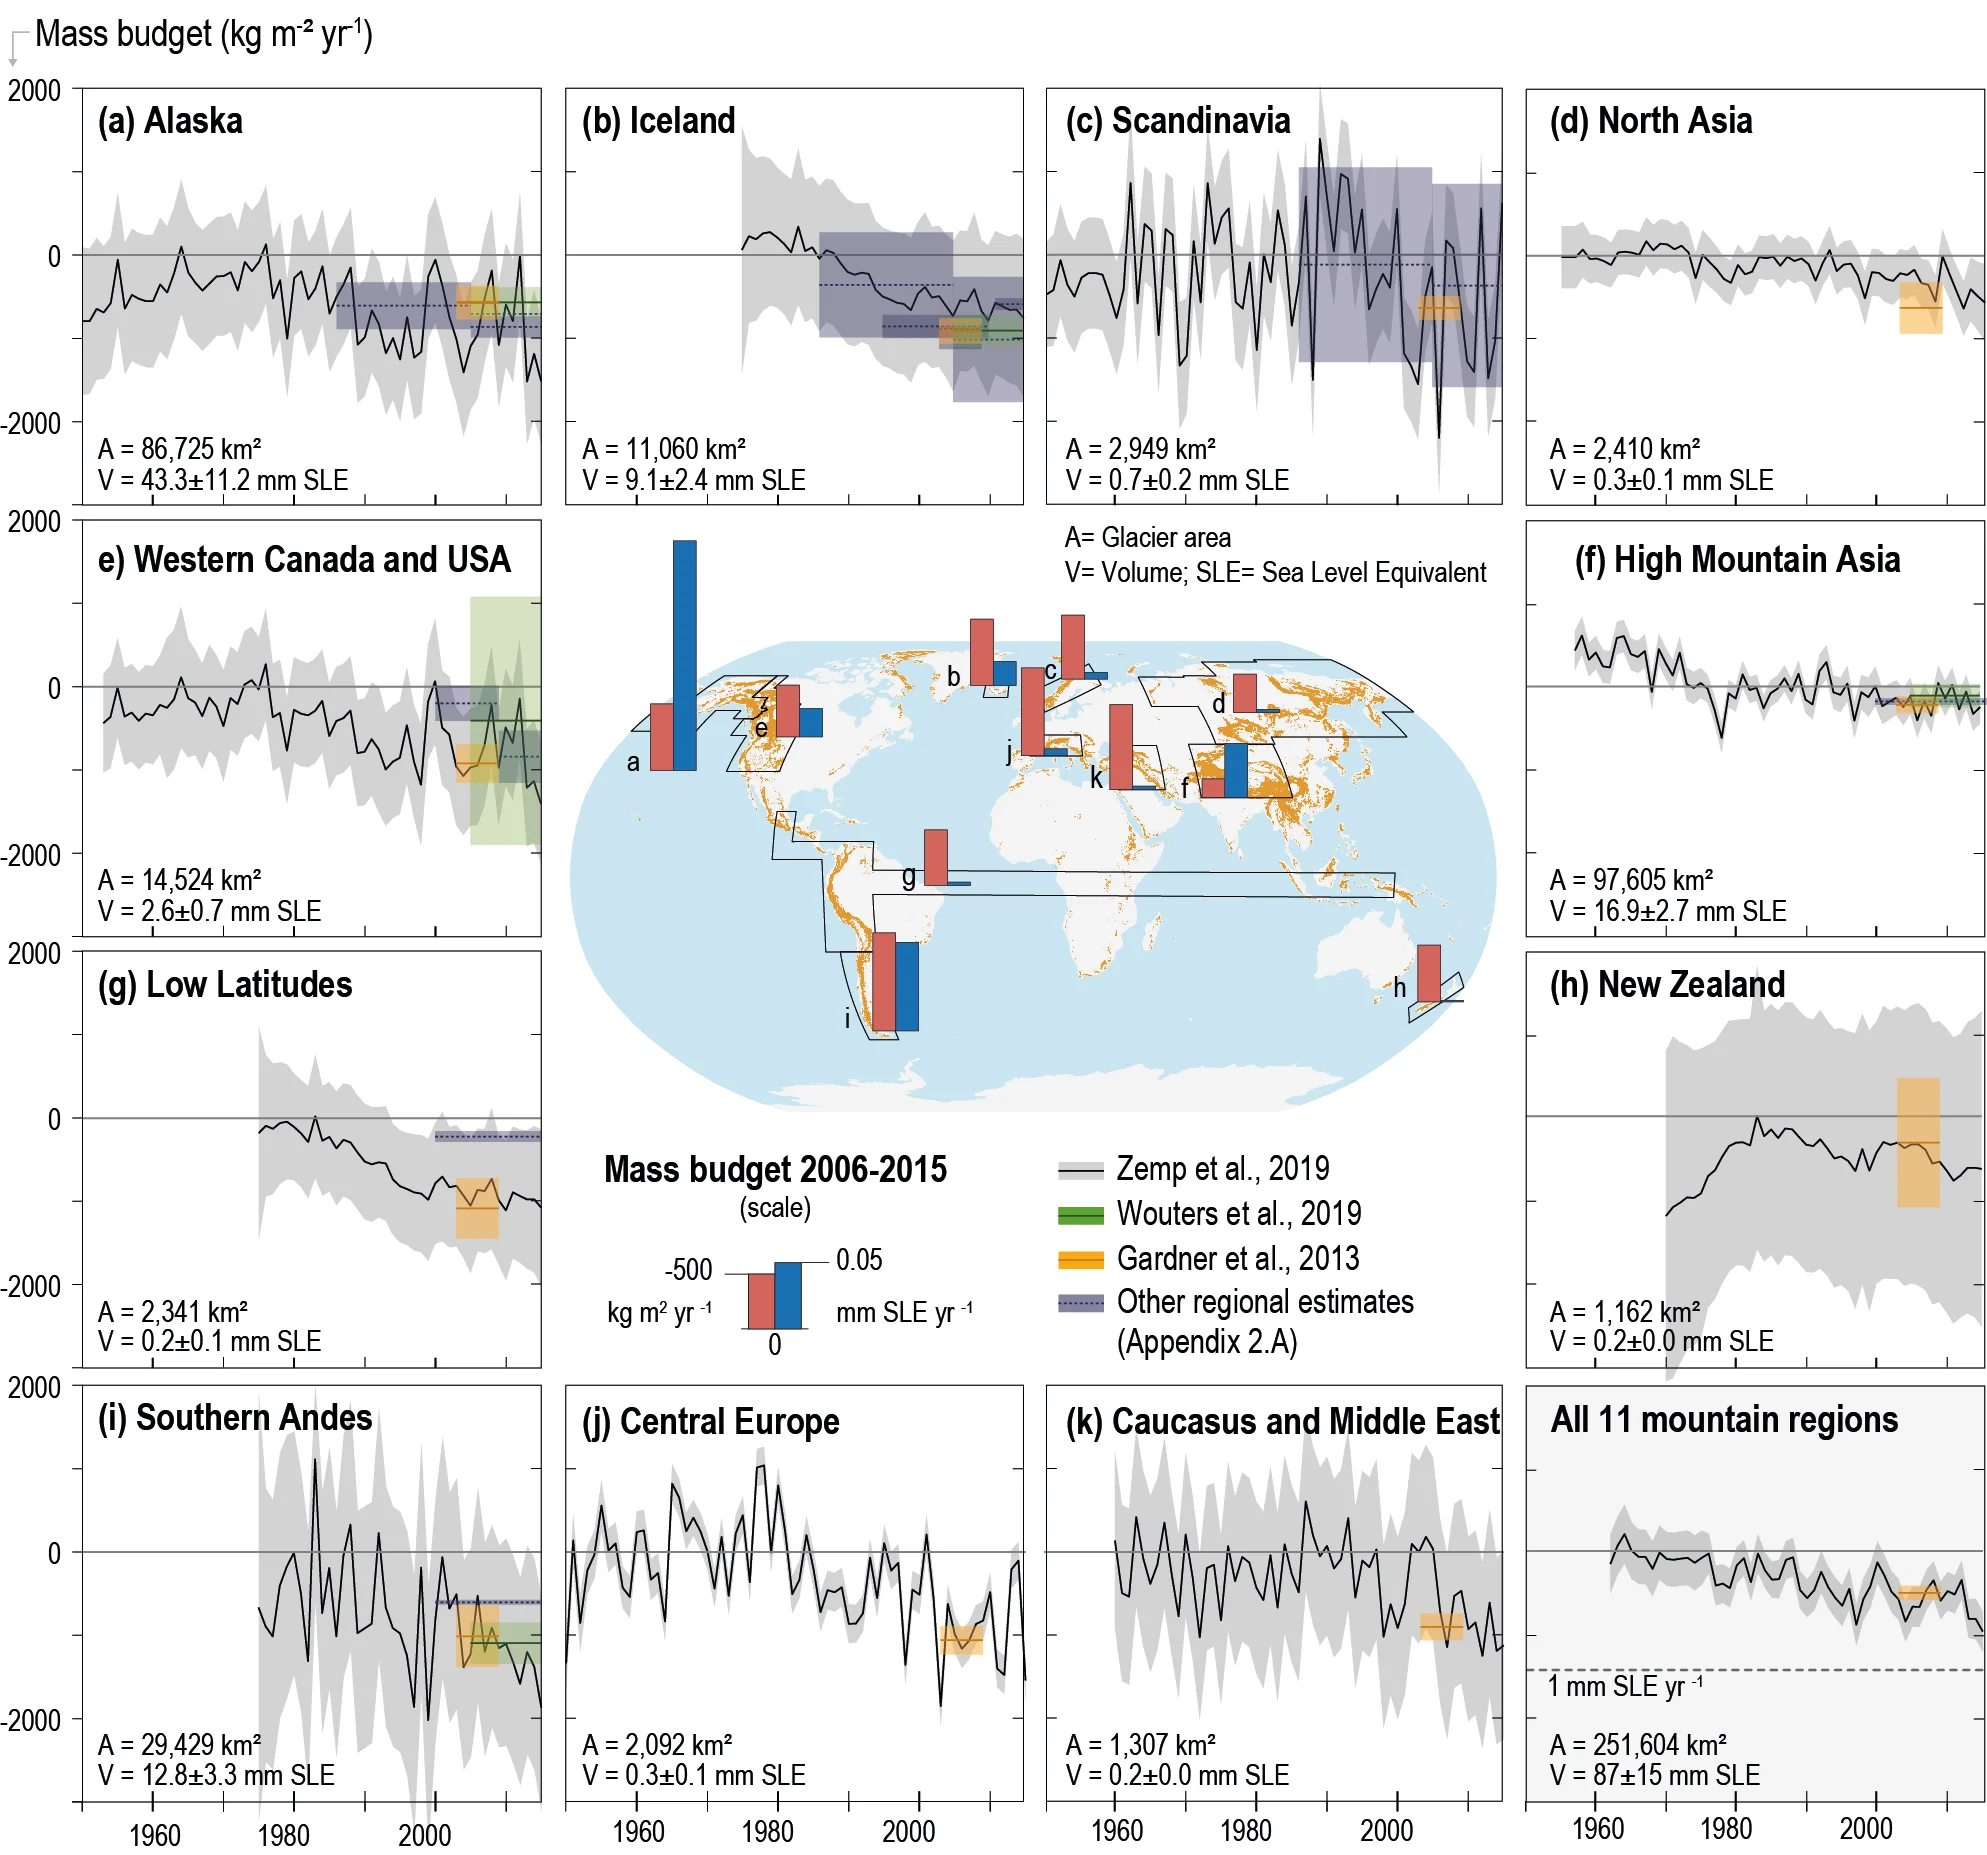
\includegraphics[width=14cm]{Figures/intro/Figure_1.png}
\caption{Glacier mass budgets for eleven different mountain regions and their combined results. Regional time series of annual mass change are based on glaciological and geodetic balances (Zemp et al., 2019). Superimposed are multi-year averages by Wouters et al. (2019) based on the Gravity Recovery and Climate Experiment (GRACE), only shown for the regions with glacier area > 3,000 km$^{2}$. Estimates by Gardner et al. (2013) were used in the IPCC 5th Assessment Report (AR5). Annual and time-averaged mass-budget estimates include the errors reported in each study. Glacier areas (A) and volumes (V) are based on RGI Consortium (2017)
and Farinotti et al. (2019), respectively. Red and blue bars on map refer to regional budgets averaged over the period 2006–2015 in units of kg m$^{–2}$ a$^{–1}$ and mm sea level equivalent (SLE) a$^{–1}$, respectively, and are derived from each region's available mass-balance estimates. \textit{Figure from IPCC's Special Report on the Ocean and Cryosphere in a Changing Climate (SROCC, 2019).}} 
\label{intro:fig1}
\end{figure*}

Mountain glaciers are predicted to lose an important fraction of their overall mass by the end of the 21$^{st}$ century, with great differences between regions \citep{hock_glaciermip_2019}. The correct assessment of future glacier evolution is essential to understand and quantify the environmental and social consequences of their retreat. Since glaciers have become an icon of climate change, accurate predictions paired with effective communication can prove a great way to raise awareness on climate change. Despite scientific efforts to precisely quantify and understand glacier retreat, the main driver of future uncertainty in long-term predictions are anthropogenic greenhouse emissions \citep{marzeion_partitioning_2020}. Scientific studies on glaciers must find their way into a wider audience in order to effectively contribute to their conservation \citep{moser_communicating_2010}. By combining an improved understanding of glacier processes with targeted communication of relevant results, we can aim at preserving our very own subject of study.  

\section{Glaciers in the French Alps}

\begin{wrapfigure}{R}{0.55\linewidth}
\centering
\includegraphics[width=8.3cm]{Figures/intro/Figure_2.pdf}
\caption{Glacierized massifs in the French Alps, with the extent of glaciers for the year 2015.}
\label{intro:fig2}
\end{wrapfigure}

The French Alps are located in the westernmost part of the European Alps, between 44º and 46º13'N and 5.08 and 7.67ºE. Their geographical location amidst the Mediterranean sea and continental Europe produces a particular climate gradient, from south-east to north-west. The southern massifs are more influenced by a Mediterranean climate, receiving less precipitation than their northern counterparts. West Atlantic fluxes bring higher amounts of precipitation to north-western massifs, whereas eastern glaciers close to the Italian border receive most precipitation from east returns \citep{durand_reanalysis_2009}. These different climatic patterns, together with altitudes ranging from sea level to 4810 m at the summit of Mont Blanc, create an array of sub-climates that influence the evolution of glaciers. A total area of 231 km$^{2}$ was covered by glaciers in the year 2015 the French Alps \citep[with 2015 update]{gardent_multitemporal_2014}.

The French Alps have been inhabited for many centuries, developing a close relationship between alpine society and mountains. As for mountain peaks, the general social attitude towards glaciers has strongly evolved in the last centuries, transitioning from disdain and terror to awe and curiosity \citep{zryd_les_2008}. This close relationship between society and glaciers has given them an important status in mountain culture, becoming symbols of identity for alpine societies throughout the European Alps. This means that the loss of glaciers has an additional social consequence in the French Alps, on top of the environmental ones found in all glacierized regions \citep{smit_exploring_2019}. 

These long-term interactions between people and glaciers resulted in some of the earliest studies and observations on glaciers in the world. From the 18$^{th}$ century, the first mountain expeditions were seen as scientific endeavours, providing valuable observations of unknown natural sites \citep{richalet_scientific_2001}. This tradition has continued ever since in the whole European Alps, with the longest observation series of glacier change in the world \citep{glamos_swiss_2019}. In France, the GLACIOCLIM national observatory is now responsible for this task, providing uninterrupted multiple glacier measurements from the field every year since the 1950's. These long-term observations, combined with the rather easy access to glaciers, provide an excellent testbed for glaciological studies. The European and French Alps are one of the regions in the world with a strongest glacier retreat (Fig. \ref{intro:fig1}), and they are also among the regions with the highest forecasted mass loss for this century \citep{marzeion_partitioning_2020}.

In many aspects, people in the French Alps have built their lives around mountains and glaciers, whose vast forecasted retreat will impact their socio-economic model \citep{mourey_evolution_2017, spandre_winter_2019}. Emblematic regions such as the Mont-Blanc massif depend on glaciers for tourism \citep{schut_sport_2013, spandre_climate_2019}, water resources and hydro-power generation  \citep{laurent_impact_2020}. Moreover, natural hazards derived from glacier retreat might potentially impact populations in valleys \citep{magnin_estimating_2020}. All these effects demand deep changes in the socio-economic model of these regions in order to correctly adapt to these changes in time. This adaptation is impossible without accurate predictions of future glacier evolution. Models can provide answers to these questions, allowing the anticipation and prioritization of actions.

\section{Modelling large-scale glacier evolution}

\emph{"At last, combining the three causes which contribute to the maintenance of glaciers, it would be interesting to arrive at the mass which is supplied to them each year; but one feels that it is only possible to have on this subject more or less probable conjectures; it is especially here that we lack and will always lack observations, which must be the first element to lead to the intelligence of nature."}.

Like an oracle, the French canon Rendu stated in 1840 what all modern glacier modellers are still struggling with. First and foremost, observations are a key element in our understanding of glacier processes. Past observations enable the creation of equations and models to represent in an approximate manner the complex behaviour of glaciers. All glacier models, independently from their approach, will have to solve the two main processes that determine the evolution of glaciers: (a) Glacier mass balance, as the consequence of the mass gained via accumulation (e.g. snowfall, avalanche deposition) and the mass lost through ablation (e.g. ice melting, calving). Mass balance can be seen as the main consequence of climate-glacier interactions \citep{benn_glaciers_2014}; (b) Glacier ice dynamics govern the movement of ice downwards due to gravity. Since ice is a viscoelastic material, this movement can occur as a combination of plastic deformation of the ice (also known as creep), sliding of ice over the bed and the deformation of the bed itself \citep{cuffey_physics_2010}. The interplay of mass balance and ice dynamics determines the advance or retreat of glaciers, as a consequence of climate and topography. Past observations of these two main processes have enabled the development of a variety of glacier models of different complexities, used to simulate glacier evolution at different geographical scales. As for any geophysical problem, the larger the study area the more simplifications are added to models. This holds especially true for glaciers, for which several parametrizations and simplifications are needed for models to operate at regional or global scale \citep[e.g.][]{marzeion_past_2012, huss_new_2015, maussion_open_2019}. 

Predicting the future of glaciers is a complex task. It demands a correct representation of past observed glacier changes, accompanied with the hypothesis that the past observed relationships will remain constant in the future. This hypothesis would not be necessary with a detailed-enough representation of the physical processes involved in glacier evolution, but a large geographical scale hinders this level of detail in current models. Most importantly, future climate and therefore glacier evolution depend on future anthropogenic greenhouse emissions, introducing large uncertainties in projections that cannot be avoided \citep{marzeion_partitioning_2020}. Therefore, the quest of the modern glacier modeller is to strike a balance between data availability, model complexity and geographical scale.

\section{Teaching machines about glaciers}
\label{intro:ml}

Regional and global glacier evolution models have been developed following a wide variety of approaches. The detailed representation of glacier processes is still a huge challenge, so modellers approach simplifications in different fashions. 

Complex physics involved in glacier processes can be simplified using empirical parametrizations, based on assumptions derived from observations. Despite their simplicity, these parametrizations often display a better performance than more complex approaches, since they are well adapted to large-scale problems where some physical processes become less important compared to others \citep{reveillet_relative_2018}. Parametrizations have been applied to both glacier mass balance (e.g. a temperature-index model) and ice dynamics (e.g. area-volume scaling, $\Delta$h parametrization), providing the tools for the vast majority of regional and global glacier evolution models \citep[e.g.][]{marzeion_past_2012, huss_new_2015, maussion_open_2019}.

\begin{figure*}[h]
\centering
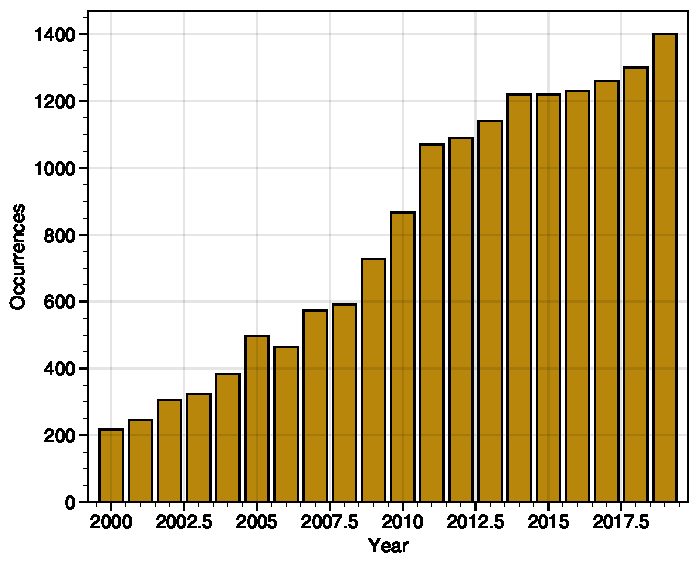
\includegraphics[width=9cm]{Figures/intro/Figure_3.pdf}
\caption{Number of scientific articles containing the words "glacier machine learning", based on queries on Google Scholar. \textit{Made with} \citet{strobel_pold87academic-keyword-occurrence_2018}.}
\label{intro:fig3}
\end{figure*} 

Alternatively, statistical models approach simplifications from a purely data-driven perspective. Relationships found in past observations can be used to create statistical models, used to analyse these relationships and performing predictions for unseen cases. Traditional linear statistical models have been applied in glaciology for more than 50 years \citep{hoinkes_glacier_1968, martin_correlation_1974}. In the last decades, statistics have seen a massive increase in both their popularity and research output with the advent of machine learning. The ever-growing amount of data stored by humans is becoming increasingly challenging to use, process and interpret, leading to the development of advanced methods in data science \citep{mjolsness_machine_2001}. As in many research fields, machine learning has made its way into glaciology (Fig.  \ref{intro:fig3}), albeit with less intensity than other fields in earth sciences such as climatology \citep[e.g.][]{liu_application_2016,ham_deep_2019,jiang_deep_2018} or oceanography \citep[e.g.][]{ducournau_deep_2016,lguensat_learning_2019}. Linear machine learning models have been applied to regression problems in order to interpret climate-glacier interactions \citep{maussion_enso_2015}, and a shallow neural network was applied to model a glacier's mass balance and length \citep{steiner_application_2005,steiner_sensitivity_2008}.  In the last years, neural networks have been revolutionized with new methods enabling the training of deep neural networks (i.e. deep learning), composed of multiple intermediate layers. This depth allows the neural networks to capture more complex non-linear patterns in data, resulting in improved performance in a wide range of problems \citep{wang_origin_2017}. Nonetheless, very few efforts have been made in this direction in glaciology in the recent years, with most recent research focusing on classification problems \citep{mohajerani_detection_2019, baumhoer_automated_2019, zhang_automatically_2019}. Classification problems offer a more straightforward problem to validate in geosciences, avoiding the tricky question of reproducing physical processes with a "black box" approach \citep{karpatne_theory-guided_2017}. Applying deep learning to geophysical regression problems is a complex task, demanding a solid validation of the results in order to avoid pitfalls related to spatiotemporal data independence \citep{roberts_cross-validation_2017}. 

\encart{The "black box" effect}{Machine learning is a relatively new research field, with a lot of complicated jargon that is in constant evolution due to the high research output of the last years. This rapid evolution, often displaying rather spectacular results in particular applications, has nonetheless been counterbalanced by a reputation that machine learning models act essentially as "black boxes". They are regarded as opaque models, taking input data, training on them in order to reproduce the patterns in the dataset, and spitting out the results without the possibility of understanding what is going on inside them. While this might be true for certain situations, this general statement is quite misleading, and it can the source of a great deal of confusion. Deep learning, being a particular family of machine learning, can often act as a black box as I am going to show in this work, but this is not the case for many other algorithms. The so-called "accuracy \textit{vs} interpretability" tradeoff tells us that, as a rule of thumb, methods with the strongest predictive power are also the most complex ones to interpret. Therefore, machine learning can still be used to interpret relationships in data, at the cost of sacrificing some predictive power \citep{riccia_machine_1997}. Nonetheless, this notion is currently being challenged by a new wave of interpretable machine learning methods, spearheaded by interpretable deep learning \citep[e.g.][]{dong_improving_2017, zhang_interpretable_2018, rackauckas_universal_2020}. These new methods, as I am going to elaborate in the last chapter, have a huge potential to overcome the current limitations of machine learning.}

In this manuscript, I introduce my attempt to apply deep learning to model glacier evolution at a regional scale. The French Alps are used as a case study, for which their evolution is studied from the late 1960's until the end of the 21$^{st}$ century. As it often happens in science, this objective was not included in my original PhD project. Initial tests with a simple statistical glacier mass balance model slowly evolved into more complex linear machine learning and eventually into deep learning. A great deal of what is included in this manuscript are the lessons learnt from numerous problems, mistakes and dilemmas that I encountered during these three years. 

\section{Modelling glacierized mountain catchments}

The correct assessment of the consequences of glacier retreat requires not only an understanding of the evolution of glaciers, but a hydrological perspective of their role at catchment scale. In the French Alps, this type of studies are only found at the scale of the whole European Alps \citep{coppola_impact_2018} or the Mont-Blanc massif \citep{laurent_impact_2020}. The J2K hydrological model \citep{krause_quantifying_2002}, developed at the University of Jena (Germany), has been applied and co-developed for many years by hydrologists in many countries, including France, in a wide variety of catchment configurations \citep{branger_investigating_2012, braud_j2000-rhone_2017, horner_information_2020}. Among these studies, a special focus was placed in glacierized catchments, with a few hydroglaciological modelling studies in Himalayan mountain catchments \citep{gao_test_2012, nepal_understanding_2014}. The current representation of glaciers in J2K takes into account a wide variety of processes, including snow evaporation, the compaction of the snow pack or even debris cover \citep{nepal_understanding_2014}. Nonetheless, the absence of glacier geometry evolution hinders its application for long-term projections in glacierized mountain catchments. Glaciers are included as static objects, acting as unchanging ice reservoirs \citep{nepal_understanding_2014}. This approach is highly problematic in the current context of rapid glacier retreat.  Other popular hydrological models in France (e.g. GR rainfall-runoff models, \cite{coron_suite_2017}) suffer from the same limitations, highlighting the gap in knowledge on the fate of glacierized catchments in the French Alps. 

In this manuscript, I introduce an attempt to solve this problem, using output data from a glacier evolution model developed during this project \citep{bolibar_alpgm_2020}, in order to take into account glacier evolution in the J2K hydrological model. Due to the unexpected turn of events during the three years of this project, a great fraction of the time was focused on machine learning applications for glacier evolution modelling (Sect. \ref{intro:ml}). This impacted the original objectives, leaving less time to work on regional hydroglaciological modelling. Therefore, efforts on hydroglaciological modelling have been focused on a technical implementation of this method in a well-documented glacierized catchment. This work provides a validated novel methodology, ready to be applied at a larger geographical scale in future studies.

\section*{Objectives of this PhD work}
\addcontentsline{toc}{chapter}{Objectives of this PhD work}

The work of my PhD has contributed to two main research axis: (a) the methods, where I introduce a first effort to apply deep learning to model glacier evolution at a regional scale, and the addition of glacier evolution into a process-based hydrological model; (b) the results, where I analyse and present the results of numerical simulations of the evolution of all glaciers in the French Alps from the late 1960's to the end of the 21$^{st}$ century. With the combination of these two axis I attempt to address the following scientific questions:
 
\begin{list}{\textbf{Question}}{}

\item \textbf{1} - Can deep learning be applied to model annual glacier mass balance changes at a regional scale? What are the benefits of using nonlinear deep learning models compared to linear machine learning?

\item \textbf{2}  - What are the annual glacier changes of all glaciers in the French Alps during the last 50 years? 

\item \textbf{3} - How will French alpine glaciers evolve during the 21$^{st}$ century? How does glacier retreat affect the climate signal on glaciers? What are the main factors that determine glacier survival in the French Alps?

\end{list}

After answering these questions during this work, a new one arose, setting the direction of future research venues:

\begin{list}{\textbf{Question}}{}

\item \textbf{4} - What are the caveats of the deep learning modelling approach used in this work? What improvements are needed to overcome these limitations for glaciological studies?

\end{list}

\section*{A short note to the reader}
\addcontentsline{toc}{chapter}{A short note to the reader}

This manuscript consists of three parts: one dedicated to regional glacier evolution modelling, another one to hydroglaciological modelling of glacierized  alpine catchments and a final one as an outlook. Part I, being the largest one, is built around three papers: two published and one in preparation. Each paper is included as a dedicated chapter, with a small preface giving the necessary context to the reader. This regional glacier modelling part follows a logical structure found in most publications: a first paper dedicated to the methods (Chapter 2), a second paper dedicated to the results of the application of this method to reconstruct past mass balance changes in the French Alps (Chapter 3), and a third paper dedicated to the future evolution of French Alpine glaciers under different scenarios of climate change (Chapter 4). Part II, dedicated to hydroglaciological modelling of glacierized catchments, is included as a single chapter (Chapter 5) with a section detailing the modelling approach, and a results section presenting the preliminary results. At last, Part III, with Chapter 6, serves as a conclusion, where various relevant topics of this manuscript are discussed and some perspectives are laid down regarding the most promising future research venues of this work.

\newpage\null\thispagestyle{empty}\newpage

\newpage \thispagestyle{empty}
%\setcounter{page}{0}
%\pagestyle{empty}

\newpage\null\thispagestyle{empty}

\part{Glaciers}

%\vspace*{\stretch{1}}
%\begin{center}
%\begin{LARGE}
%\textbf{Part I: Glaciers}
%\end{LARGE}
%\end{center}
%\vspace*{\stretch{2}}

\chapter{Deep learning applied to glacier evolution modelling}
\label{chap:methods}

\begin{flushright}
\begin{small}
\textit{All models are wrong, but some are useful.}\\
George Box
\end{small}
\end{flushright}

\section*{Preface}

\section{Abstract}
We present a novel approach to simulate and reconstruct annual glacier-wide surface mass balance (SMB) series based on a deep artificial neural network (\textit{i.e.} deep learning). This method has been included as the SMB component of an open-source regional glacier evolution model. While most glacier models tend to incorporate more and more physical processes, here we take an alternative approach by creating a parameterized model based on data science. Annual glacier-wide SMBs can be simulated from topo-climatic predictors using either deep learning or Lasso (regularized multilinear regression), whereas the glacier geometry is updated using a glacier-specific parameterization. We compare and cross-validate our nonlinear deep learning SMB model against other standard linear statistical methods on a dataset of 32 French alpine glaciers. Deep learning is found to outperform linear methods, with improved explained variance (up to +64\% in space and +108\% in time) and accuracy (up to +47\% in space and +58\% in time), resulting in an estimated \(r^2\) of 0.77 and RMSE of 0.51 m.w.e. Substantial nonlinear structures are captured by deep learning, with around 35\% of nonlinear behaviour in the temporal dimension. For the glacier geometry evolution, the main uncertainties come from the ice thickness data used to initialize the model. These results should encourage the use of deep learning in glacier modelling as a powerful nonlinear tool, capable of capturing the nonlinearities of the climate and glacier systems, that can serve to reconstruct or simulate SMB time series for individual glaciers in a whole region for past and future climates. 


\section{Introduction} \label{methods:intro}

Glaciers are arguably one of the most important icons of climate change, being climate proxies which can depict the evolution of climate for the global audience \citep{ipcc_climate_2018}. In the coming decades, mountain glaciers will be some of the most important contributors to sea level rise and will most likely drive important changes in the hydrological regime of glaciarized catchments \citep{beniston_european_2018, vuille_rapid_2018, hock_glaciermip_2019}. The reduction in ice volume may produce an array of hydrological, ecological and economic consequences in mountain regions which requires to be properly predicted. These consequences will strongly depend on the future climatic scenarios, which will determine the timing and magnitude for the transition of hydrological regimes \citep{huss_global-scale_2018}. Understanding these future transitions is key for societies to adapt to future hydrological and climate configurations. 

Glacier and hydro-glaciological models can help answer these questions, giving several possible outcomes depending on multiple climate scenarios. (a) Surface mass balance (SMB) and (b) glacier dynamics both need to be modelled to understand glacier evolution on regional and sub-regional scales. Models of varying complexity exist for both processes. In order to model these processes at large scale (\textit{i.e.} on several glaciers at a catchment scale), some compromises need to be made, which can be approached in different ways:

(a) Regarding SMB:

\begin{enumerate}
\item Empirical models, like the temperature-index model \citep[e.g.][]{hock_temperature_2003}, simulate glacier SMB through empirical relationships between air temperature and melt and snow accumulation. 
\item Statistical or machine learning models describe and predict glacier SMB based on statistical relationships found in data from a selection of topographical and climate predictors \citep[e.g.][]{martin_correlation_1974, steiner_application_2005}.
\item Physical and Surface Energy Balance (SEB) models take into account all energy exchanges between the glacier and the atmosphere, and can simulate the spatial and temporal variability of snowmelt and the changes in albedo \citep[e.g.][]{gerbaux_surface_2005}.
\end{enumerate}

(b) Regarding glacier dynamics:

\begin{enumerate}
\item Parameterized models do not explicitly resolve any physical processes, but implicitly take them into account using parameterizations, based on statistical or empirical relationships, in order to modify the glacier geometry. This type of models range from very simple statistical models \citep[e.g.][]{carlson_accounting_2014} to more complex ones based on different approaches, such as a calibrated equilibrium-line altitude (ELA) model \citep[e.g.][]{zemp_alpine_2006}, a glacier retreat parameterization specific for glacier size groups \citep{huss_new_2015} or volume/length-area scaling \citep[e.g.][]{marzeion_past_2012, radic_regional_2014}. 
\item Process-based models, like GloGEMflow \citep[e.g.][]{zekollari_modelling_2019} and OGGM \citep[e.g.][]{maussion_open_2019}, approximate a number of glacier physical processes involved in ice flow dynamics using the shallow ice approximation. 
\item Physics-based models, like the finite elements Elmer/Ice model \citep[e.g.][]{gagliardini_capabilities_2013}, approach glacier dynamics by explicitly simulating physical processes and solving the full Stokes equations \citep[e.g.][]{jouvet_numerical_2009, reveillet_simulations_2015}. 
\end{enumerate}

At the same time, the use of these different approaches strongly depend on available data, whose spatial and temporal resolutions have an important impact on the results’ quality and uncertainties \citep[e.g.,][]{reveillet_relative_2018}. Parameterized glacier dynamics models and empirical and statistical SMB models require a reference or training dataset to calibrate the relationships, which can then be used for projections with the hypothesis that relationships remain stationary in time. On the contrary, process-based and specially physics-based glacier dynamics and SMB models have the advantage of representing physical processes, but they require larger datasets at higher spatial and temporal resolutions with a consequently higher computational cost \citep{reveillet_relative_2018}. For SMB modelling, meteorological reanalyses provide an attractive alternative to sparse point observations, although their spatial resolution and suitability to complex high-mountain topography are often not good enough for high-resolution physics-based glacio-hydrological applications. However, parameterized models are much more flexible, equally dealing with fewer and coarser meteorological data as well as the state of the art reanalyses, which allows to work at resolutions much closer to glaciers’ scale and to reduce uncertainties. The current resolution of climate projections is still too low to adequately drive most glacier physical processes, but the ever-growing datasets of historical data are paving the way for the training of parameterized machine learning models. 

In glaciology, statistical models have been applied for more than half a century, starting with simple multiple linear regressions on few meteorological variables \citep{hoinkes_glacier_1968, martin_correlation_1974}. Statistical modelling has made enormous progress in the last decades, specially thanks to the advent of machine learning. Compared to other fields in geosciences, such as oceanography \citep[e.g.,][]{ducournau_deep_2016, lguensat_eddynet:_2018}, climatology \citep[e.g.,][]{rasp_deep_2018, jiang_deep_2018} and hydrology \citep[e.g.,][]{marcais_prospective_2017, shen_transdisciplinary_2018}, we believe that the glaciological community has not yet exploited the full capabilities of these approaches. Despite this fact, a number of studies have taken steps towards statistical approaches. \citet{steiner_application_2005} pioneered the very first study to use artificial neural networks (ANNs) in glaciology to simulate mass balances of the Grosse Aletschgletscher in Switzerland. They showed that a nonlinear model is capable of better simulating glacier mass balances compared to a conventional stepwise multiple linear regression. Furthermore, they found a significant nonlinear part within the climate/glacier mass balance relationship. This work was continued in \citet{steiner_sensitivity_2008} and \citet{nussbaumer_reseau_2012} for the simulation of glacier length instead of mass balances. Later on, \citet{maussion_enso_2015} developed an empirical statistical downscaling tool based on machine learning in order to retrieve glacier surface energy and mass balance (SEB/SMB) fluxes from large-scale atmospheric data. They used different machine learning algorithms, but all of them were linear, which are not necessarily the most suitable for modelling the nonlinear climate system \citep{houghton_climate_2001}. Nonetheless, more recent developments in the field of machine learning and optimization enabled the use of deeper network structures than the 3-layer ANN of \citet{steiner_application_2005}. These deeper ANNs, which remain unexploited in glaciology, allow to capture more nonlinear structures in the data even for relatively small datasets  \citep{ingrassia_neural_2005, olson_modern_2018}. 

Here, we present a parameterized regional open-source glacier model: the ALpine Parameterized Glacier Model \cite[ALPGM,][]{bolibar_jordibolibar/alpgm:_2019}. When most glacier evolution models tend to incorporate more and more physical processes in SMB or ice dynamics \citep[e.g.,][]{maussion_open_2019, zekollari_modelling_2019}, ALPGM takes an alternative approach based on data science for SMB modelling and parameterizations for glacier dynamics simulation. ALPGM simulates annual glacier-wide SMB and the evolution of glacier volume and surface area over time scales from a few years to a century at a regional scale. Glacier-wide SMBs are computed using a deep ANN, fed by several topographical and climatic variables, an approach which is compared to different linear methods in the present paper. In order to distribute these annual glacier-wide SMBs and to update the glacier geometry, a refined version of the $\Delta$h methodology \citep[e.g.,][]{huss_modelling_2008} is used, for which we dynamically compute glacier-specific $\Delta$h functions. In order to validate this approach, we use a case study with 32 French alpine glaciers for which glacier-wide annual SMBs are available over the period 1984-2014 and 1959-2015 for certain glaciers. High resolution meteorological reanalyses for the same time period are used \citep[SAFRAN,][]{durand_reanalysis_2009} while the initial ice thickness distribution of glaciers are taken from \citet{farinotti_consensus_2019}, for which we performed a sensitivity analysis based on field observations.

In the next section, we present an overview of the proposed glacier evolution model framework with a detailed description of the two components used to simulate the annual glacier-wide SMB and the glacier geometry update. Then, a case study using French alpine glaciers is presented, which enables to illustrate an example of application of the proposed framework including a rich dataset, the parameterized functions, as well as the results and their performance. In the end, several aspects regarding machine and deep learning modelling in glaciology are discussed, from which we make some recommendations and draw the final conclusions.


\section{Model overview and methods} \label{methods:methods}

In this section we present an overview of the ALPGM glacier model. Moreover, the two components of this model are presented in detail: the Glacier-wide SMB Simulation component and the Glacier Geometry Update component.

\subsection{Model overview and workflow} \label{methods:methods:workflow}

ALPGM is an open-source glacier model coded in Python. The source code of the model is accessible in the project repository (see Code availability). It is structured in multiple files which execute specific separate tasks. The model can be divided into two main components: (1) the Glacier-wide SMB Simulation and (2) the Glacier Geometry Update. The Glacier-wide SMB Simulation component is based on machine learning, taking both meteorological and topographical variables as inputs. The Glacier Geometry Update component generates the glacier-specific parameterized functions and modifies annually the geometry of the glacier (\textit{e.g.} ice thickness distribution, glacier outline) based on the glacier-wide SMB models generated by the Glacier-wide SMB simulation component.

\begin{figure*}[t]
\centering
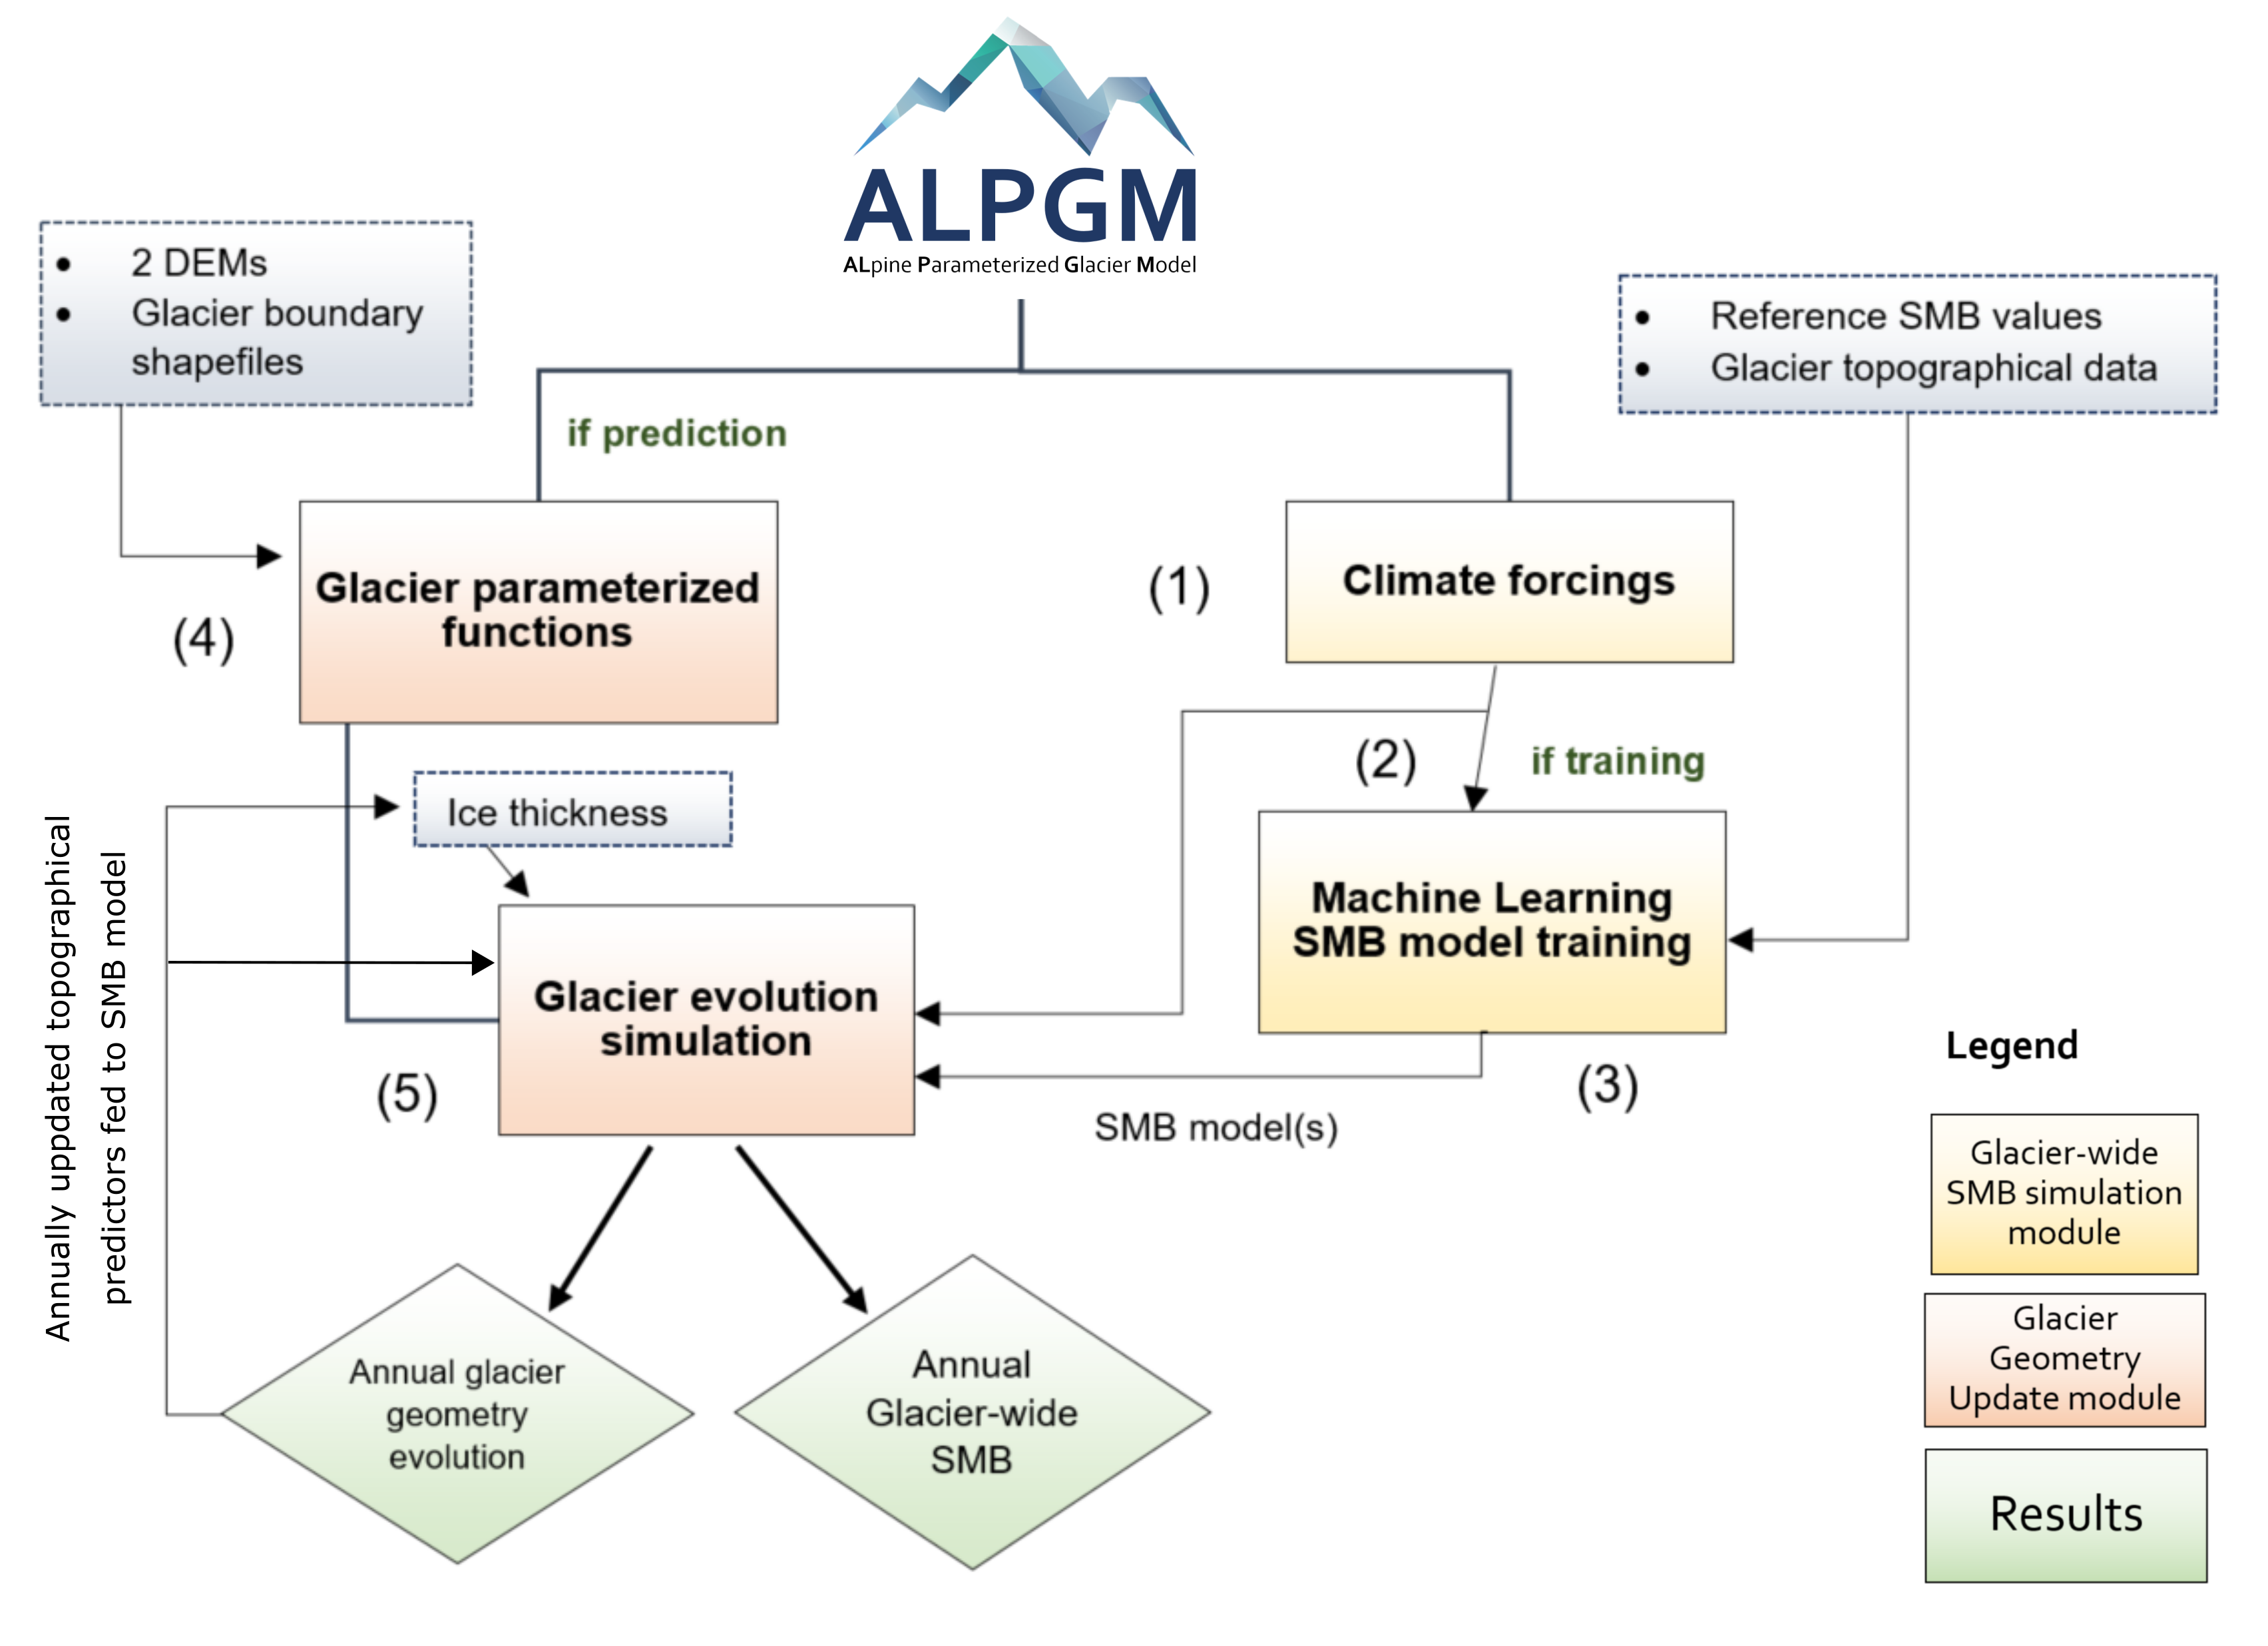
\includegraphics[width=14cm]{Figures/methods/Figure_1.png}
\caption{ALPGM structure and workflow}
\label{methods:fig1}
\end{figure*}

Figure \ref{methods:fig1} presents ALPGM’s basic workflow. The workflow execution can be configured via the model interface, allowing to run or skip any of the following steps:

\begin{enumerate}
\item The meteorological forcings are preprocessed in order to extract the necessary data closest to each glacier’s centroid. The meteorological features are stored in intermediate files in order to reduce computation times for future runs, automatically skipping this preprocessing step when the files have already been generated.
\item The SMB machine learning component retrieves the preprocessed climate predictors from the stored files, retrieves the topographical predictors from the multitemporal glacier inventories, and then it assembles the training dataset by combining all the necessary topo-climatic predictors. A machine learning algorithm is chosen for the SMB model, which can be loaded from a previous run or it can be trained again with a new dataset. Then, the SMB model(s) are trained with the full topo-climatic dataset. These model(s) are stored in intermediate files, allowing to skip this step for future runs.
\item Performances of the SMB models can be evaluated with a leave-one-glacier-out (LOGO) or a leave-one-year-out (LOYO) cross-validation. This step can be skipped when using already established models. Basic statistical performance metrics are given for each glacier and model, as well as plots with the simulated cumulative glacier-wide SMBs compared to their reference values with uncertainties for each of the glaciers from the training dataset.
\item The Glacier Geometry Update component starts with the generation of the glacier specific parameterized functions, using a raster containing the difference of the two pre-selected digital elevation models (DEMs) covering the study area for two separate dates, as well as the glacier contours. These parameterized functions are then stored in individual files to be used in the final simulations.
\item Once all previous steps have been run, the glacier evolution simulations are launched. For each glacier, the initial ice thickness and DEM rasters and the glacier geometry update function are retrieved. Then, in a loop, for every glacier and year, the topographical data is computed from these raster files. The climate predictors at the glacier’s current centroid are retrieved from the climate data (e.g. reanalysis or projections) and with all this data the input topo-climatic data for the glacier-wide SMB model is assembled. Afterwards, the glacier-wide SMB for this glacier and year is simulated, which combined with the glacier-specific geometry update function allows to update the glacier’s ice thickness and DEM rasters. This process is repeated in a loop, therefore updating the glacier’s geometry with an annual timestep and taking into account the glacier’s morphological and topographical changes in the glacier-wide SMB simulations. For the simulation of the following year’s SMB, the previously updated ice thickness and DEM rasters is used to re-compute the topographical parameters, which in turn are used as input topographical predictors for the glacier-wide SMB machine learning model.  If all the ice thickness raster pixels of a glacier become zero, the glacier is considered as disappeared and is removed from the simulation pipeline. For each year, multiple results are stored in data files as well as the raster DEM and ice thickness values for each glacier. 
\end{enumerate}

\subsection{Glacier-wide surface mass balance simulation} \label{methods:methods:SMB}
Annual glacier-wide SMBs are simulated using machine learning. Due to the regional characteristics and specificities of topographical and climate data, this glacier-wide SMB modelling method is, for now, a regional approach.

\subsubsection{Selection of explanatory topographical and climatic variables} 

In order to narrow down which topographical and climatic variables best explain glacier-wide SMB in a given study area, a literature review as well as a statistical sensitivity analysis are performed. Typically used topographical predictors are longitude, latitude, glacier slope and mean altitude. As for meteorological predictors, cumulative positive degree days (CPDD), but also mean monthly temperature, snowfall and possibly other variables that influence the surface energy budget are often used in the literature. Examples of both topographic and meteorological predictors can be found in the case study in Sect. \ref{methods:case_study}. A way to prevent biases when making predictions with different climate data is to work with anomalies, calculated as differences of the variable with respect to its average value over a chosen reference period. 

For the machine learning training, the relevant predictors must be selected, so we perform a sensitivity study of the annual glacier-wide SMB to topographical and climatic variables over the study training period. This can be performed with individual linear regressions between each variable and glacier-wide SMB data. After identification of the topographical and climatic variables that can potentially explain annual glacier-wide SMB variability for the region of interest, a training dataset is built. An effective way of expanding the training dataset in order to dig deeper into the available data is to combine the climatic and topographical input variables \citep{weisberg_applied_2014}. Such combinations can be expressed following equation \ref{eq:1}

\begin{equation} \label{eq:1}
SMB_{g, y}=f(\hat{\Omega}, \hat{C})+\varepsilon_{g, y}
\end{equation}

Where $\hat{\Omega}$ is a vector of the selected topographical predictors, $\hat{C}$ is a vector with the selected climatic features and $\varepsilon_{g, y}$ is the residual error for each annual glacier-wide SMB value, $SMB_{g, y}$.

Once the training dataset is created, different algorithms $f$ (two linear and one nonlinear, for the case of this study) can be chosen to create the SMB model: (1) OLS (Ordinary Least Squares) all-possible multiple linear regressions; (2) Lasso (Least absolute shrinkage and selection operator) \citep{tibshirani_regression_1996}; and (3) a deep Artificial Neural Network (ANN). ALPGM uses some of the most popular machine learning Python libraries: StatsModels \citep{seabold_statsmodels:_2010}, Scikit-learn \citep{pedregosa_scikit-learn:_2012} and Keras \citep{chollet_keras_2015} with a TensorFlow backend. The overall workflow of the machine learning glacier-wide SMB model production in ALPGM is summarized in Fig. \ref{methods:fig2}.  

\begin{figure}[t]
\centering
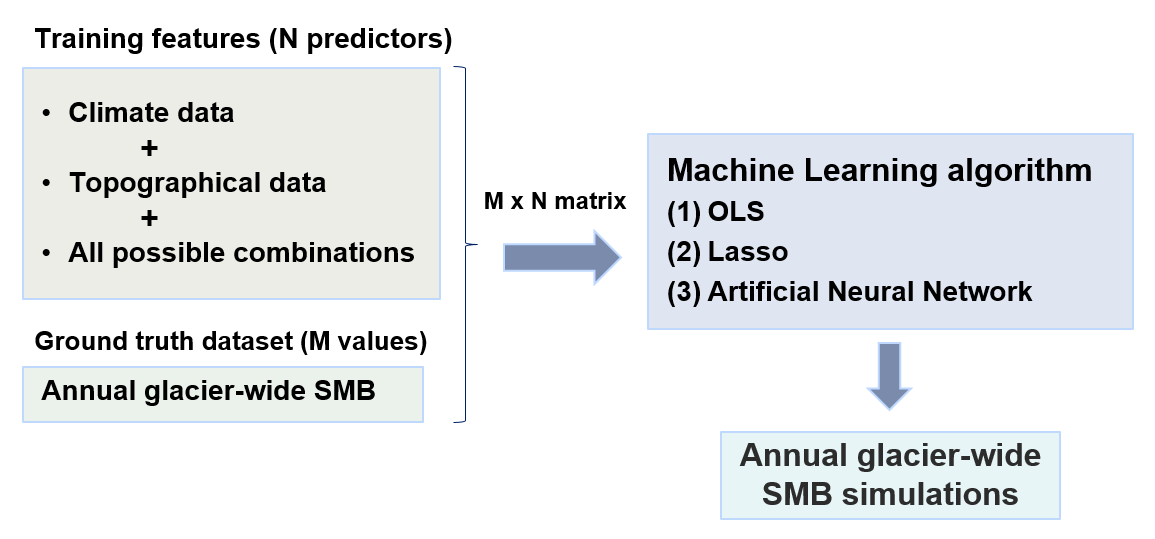
\includegraphics[width=9cm]{Figures/methods/Figure_2.png}
\caption{Glacier-wide SMB simulation component workflow. Machine learning models are dynamically created based on training data}
\label{methods:fig2}
\end{figure}

\subsubsection{All-possible multiple linear regressions} \label{methods:methods:ols}

With the ordinary least squares (OLS) all-possible multiple linear regressions, we attempt to find the best subset of predictors in Eq. \ref{eq:1} based on the resulting \(r^2\) adjusted, while at the same time avoiding overfitting \citep{hawkins_problem_2004} and collinearity, and limiting the complexity of the model. As its name indicates, the goal is to minimize the residual sum of squares for each subset of predictors \citep{hastie_elements_2009}. $n$ models are produced by selecting all possible subsets of $k$ predictors. It is advisable to narrow down the number of predictors for each subset in the search to reduce the computational cost. Models with low performance are filtered out, keeping only models with highest \(r^2\) adjusted possible, a variance inflation factor ($VIF$) < 1.2 and a p-value < 0.01/$n$ (in order to ensure the Bonferroni correction). Retained models are combined by averaging their predictions, thereby avoiding the pitfalls related to stepwise single model selection \citep{whittingham_why_2006}. These criteria ensure that the models explain as much variability as possible, avoid collinearity and are statistically significant. 

\subsubsection{Lasso} \label{methods:methods:lasso}

The Lasso (Least absolute shrinkage and selection operator) \citep{tibshirani_regression_1996} is a shrinkage method which attempts to overcome the shortcomings of the simpler step-wise and all-possible regressions. In these two classical approaches, predictors are discarded in a discrete way, giving subsets of variables which have the lowest prediction error. However, due to its discrete selection, these different subsets can exhibit high variance, which does not reduce the prediction error of the full model. The Lasso performs a more continuous regularization by shrinking some coefficients and setting others to zero, thus producing more interpretable models \citep{hastie_elements_2009}. Because of its properties, it strikes a balance between subset selection (like all-possible regressions) and Ridge regression \citep{hoerl_ridge_1970}. All input data is normalized by removing the mean and scaling to unit variance. In order to determine the degree of regularisation applied to the coefficients used in the linear OLS regression, an alpha parameter needs to be chosen using cross-validation. ALPGM performs different types of cross-validations to choose from: the Akaike Information Criterion (AIC), the Bayes Information Criterion (BIC) and a classical cross-validation with iterative fitting along a regularization path (used in the case study). Alternatively, a Lasso model with Least Angle Regression, also known as Lasso Lars \citep{tibshirani_least_2004}, can also be chosen with a classical cross-validation. 

\subsubsection{Deep artificial neural networks} \label{methods:methods:ann}

Artificial neural networks (ANNs) are nonlinear statistical models inspired by biological neural networks \citep{fausett_fundamentals_1994, hastie_elements_2009}. A neural network is characterized by: (1) the architecture or pattern of connections between units and the number of layers (input, output and hidden layers); (2) the optimizer: which is the method for determining the weights of the connections between units; and (3) its (usually nonlinear) activation functions \citep{fausett_fundamentals_1994}. When ANNs have more than one hidden layer (\textit{e.g.} Fig. \ref{methods:fig3}), they are referred to as deep ANNs or deep learning. The description of neural networks is beyond the scope of this study, so for more details and a full explanation please refer to \citet{fausett_fundamentals_1994}, \citet{hastie_elements_2009}, as well as \citet{steiner_application_2005, steiner_sensitivity_2008} where the reader can find a thorough introduction to the use of ANNs in glaciology. ANNs gained recent interest thanks to improvements of optimization algorithms enabling the training of deep neural networks, that lead to better representation of complex data patterns. As their learnt parameters are difficult to interpret, ANN are adequate tools when the quality of predictions prevails over the interpretability of the model (the latter likely involving causal inference, sensitivity testing or modelling of ancillary variables). This is precisely the case in our study context here, where abundant knowledge about glacier physics further helps choosing adequate variables as input to deep learning. Their ability to model complex functions of the input parameters makes them particularly suitable for modelling complex nonlinear systems such as the climate system \citep{houghton_climate_2001} and glacier systems \citep{steiner_application_2005}.

ALPGM uses a feedforward fully-connected ANN (Fig. \ref{methods:fig3}). In such an architecture, the processing units - or neurons - are grouped into layers where all the units of a given layer are fully connected to all units of the next layer. The flow of information is directional, from the input layer (\textit{i.e.}. in which each neuron corresponds to one of the N explanatory variables) to the output neuron (\textit{i.e.}. corresponding to the target variable of the model, the SMB). For each connection of the ANN, weights are initialized in a random fashion following a specific distribution (generally centred around 0). In each unit of each hidden layer, the weighted values are summed before going through a nonlinear activation function, responsible for introducing the nonlinearities in the model. Using a series of iterations known as epochs, the ANN will try to minimize a specific loss function (the mean squared error (MSE) in our case) comparing the processed values of the output layer with the ground truth ($y$). In order to avoid falling into local minima of the loss function, some regularisation is needed to prevent the ANN from overfitting \citep{hastie_elements_2009}.  To prevent overfitting during the training process (\textit{i.e.}. to increase the ability of the model to generalize to new data), we used a classical regularization method called dropout, consisting in training iteratively smaller subparts of the ANN by randomly disconnecting a certain amount of connections between units. The introduction of Gaussian noise at the input of the ANN also helped to generalize, as it performs a similar effect to data augmentation. The main consequence of regularisation is generalization, for which the produced model is capable of better adapting to different configurations of the input data. 

\begin{figure*}[t]
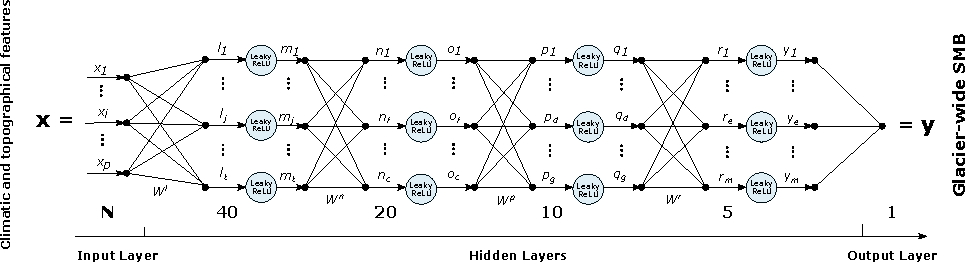
\includegraphics[width=15cm]{Figures/methods/Figure_3.pdf}
\caption{Deep Artificial Neural Network architecture used in ALPGM. The numbers indicate the number of neurons in each layer}
\label{methods:fig3}
\end{figure*}

The hyperparameters used to configure the ANN are determined using cross-validation, in order to find the best performing combination of number of units, hidden layers, activation function, learning rate and regularisation method. Due to the relatively small size of our dataset, we encountered the best performances with a quite small deep ANN, with a total of 6 layers (4 hidden layers) with a ($N$, 40, 20, 10, 5, 1) architecture (Fig. \ref{methods:fig3}), where $N$ is the number of selected features. Since the ANN already performs all the possible combinations between features (predictors), we use a reduced version of the training matrix from Eq. \ref{eq:1}, with no combination of climatic and topographical features. Due to the relatively small size of the architecture, the best dropout rates are small \citep{srivastava_dropout:_2014}, and range between 0.3 and 0.01 depending on the number of units of each hidden layer. Leaky ReLUs have been chosen as the activation function, because of their widespread reliability and the fact they help prevent the “dead ReLU” problem, where certain neurons can stop “learning” \citep{xu_empirical_2015}. The He uniform initialization \citep{he_delving_2015} has been used as it is shown to work well with Leaky ReLUs, and all unit bias were initialized to zero. In order to optimize the weights of the gradient descent, we used the RMSprop optimizer, for which we fine-tuned the learning rate, obtaining the best results at 0.0005 in space and 0.02 in time. Each batch was normalized before applying the activation function in order to accelerate the training \citep{ioffe_batch_2015}. 

Like for many other geophysical processes found in nature, extreme annual glacier-wide SMB values occur much less often than average values, approximately following an unbounded Gumbel-type distribution \citep{thibert_causes_2018}. From a statistical point of view, this means that ANN will “see” few extreme values and will accord less importance to them. For future projections in a warmer climate, extreme positive glacier-wide SMB balances should not be the main concern of glacier models. However, extreme negative annual glacier-wide SMB values should likely increase in frequency, so it is in the modeller’s interest to reproduce them as well as possible. Setting the sample weights as the inverse of the probability density function during the ANN training can partly compensate for the imbalance of a dataset. This boosts the performance of the model for the extreme values, at the cost of sacrificing some performance on more average values, which can be seen as a \(r^2\)/RMSE trade-off (Fig. \ref{methods:fig6} and \ref{methods:fig9} from the case study). The correct setting of the sample weights allows the modeller to adapt the ANN to each dataset and application. 

\subsection{Glacier geometry update} \label{methods:methods:deltah}

Since the first component of ALPGM simulates annual glacier-wide SMBs, these changes in mass need to be redistributed over the glacier surface-area in order to reproduce glacier dynamics. This redistribution is applied using the $\Delta$h parameterization. The idea was first developed by \citet{johannesson_timescale_1989} and then adapted and implemented by \citet{huss_modelling_2008}. The main idea behind it is to use two or more DEMs covering the study area. These DEMs should have dates covering a period long enough (which will be later discussed in detail). By subtracting them, the changes in glacier surface elevation over time can be computed, which corresponds to a change in thickness (considering no basal erosion). Then, these thickness changes are normalized and considered as a function of the normalized glacier altitude. This $\Delta$h function is specific for each glacier and represents the normalized glacier thickness evolution over its altitudinal range. One advantage of such a parametrized approach is that it implicitly considers the ice flow which redistributes the mass from the accumulation to the ablation area. In order to make the glacier volume evolve in a mass-conserving fashion, we apply this function to the annual glacier-wide SMB values in order to scale and distribute its change in volume. 

As discussed in \citet{vincent_future_2014}, the time period between the two DEMs used to calibrate the method needs to be long enough to show important ice thickness differences. The criteria will of course depend on each glacier and each period, but it will always be related to the achievable signal-to-noise ratio. \citet{vincent_future_2014} concluded that for their study on the Mer de Glace glacier (28.8 \(km^2\), mean altitude = 2868 m.a.s.l.) in the French Alps, the 2003-2008 period was too short, due to the delayed response of glacier geometry to a change in surface mass balance. Indeed, the results for that 5-year period diverged from the results from longer periods. Moreover, the period should be long enough to be representative of the glacier evolution, which will often encompass periods with strong ablation and others with no retreat or even with positive SMBs. 

Therefore, by subtracting the two DEMs, the ice thickness difference is computed for each specific glacier. These values can then be classified by altitude, thus obtaining an average glacier thickness difference for each pixel altitude. As a change to previous studies \citep{vincent_future_2014, huss_new_2015, hanzer_projected_2018, vincent_declin_2019}, we no longer work with altitudinal transects, but with individual pixels. In order to filter noise and artefacts coming from the DEM raster files, different filters are applied to remove outliers and pixels with unrealistic values, namely at the border of glaciers or where the surface slopes are high (refer to Supplements for detailed information). Our methodology thus allows to better exploit the available spatial information based on its quality, and not on arbitrary location within transects. 

\section{Case study: French alpine glaciers} \label{methods:case_study}
\subsection{Data} \label{methods:case_study:data}

All data used in this case study is based on the French Alps (Fig. \ref{methods:fig4}), located in the westernmost part of the European Alps, between 5.08° and 7.67°E, and 44° and 46°13’N. This region is particularly suited for the validation of a glacier evolution model because of the wealth of available data. Moreover, ALPGM has been developed as part of a hydro-glaciological study to understand the impact of the retreat of French alpine glaciers in the Rhône river catchment (97,800 \(km^2\)). 

\subsubsection{Glacier-wide surface mass balance }

An annual glacier-wide SMB dataset, reconstructed using remote sensing based on changes in glacier volume and the snow line altitude, is used \citep{rabatel_spatio-temporal_2016}. This dataset is constituted by annual glacier-wide SMB values for 30 glaciers in the French Alps (Fig. \ref{methods:fig4}) for 31 years, between 1984-2014. The great variety in topographical characteristics of the glaciers included in the dataset, with a good coverage of the three main clusters or groups of glaciers in the French Alps (Fig. \ref{methods:fig4}), makes them an ideal training dataset for the model. Each of the clusters represents a different setup of glaciers with different contrasting latitudes (Écrins and Mont-Blanc), longitudes (Écrins and Vanoise), glacier size (smaller glaciers in Écrins and Vanoise $vs$ larger ones in Mont-Blanc) and climatic characteristics with a Mediterranean influence towards the south of the study region. For more details regarding this dataset refer to \citet{rabatel_spatio-temporal_2016}. Data from the Mer de Glace, Saint-Sorlin, Sarennes and Argentière glaciers is also used, coming from field observations from the GLACIOCLIM observatory. For some of these glaciers, glacier-wide SMB values are available since 1949, although only values from 1959 onwards were used to match the meteorological reanalysis. This makes a total of 32 glaciers (Argentière and Saint-Sorlin glaciers belonging to the two datasets), representing 1048 annual glacier-wide SMB values (taking into account some gaps in the dataset).

\subsubsection{Topographical glacier data and altimetry} 

The topographical data used for the training of the glacier-wide SMB machine learning models is taken from the multitemporal inventory of the French Alps glaciers \citep[e.g.,][]{gardent_multitemporal_2014} partly available through the GLIMS Glacier Database \citep{glims_and_nsidc_global_2005}. We worked with the 1967, 1985, 2003 and 2015 inventories \citep[with 2015 update]{gardent_multitemporal_2014}. Between these dates, the topographical predictors are linearly interpolated. On the other hand, in the glacier evolution component of ALPGM (Fig. \ref{methods:fig1}, step 5), the topographical data is re-computed every year for each glacier from the evolving and annually updated glacier-specific ice thickness and DEM rasters (Sect. \ref{methods:case_study:data}). Since these raster files are estimates for the year 2003 (\citet{farinotti_consensus_2019} for the ice thickness), the full glacier evolution simulations can start the earliest at this date. For the computation of the glacier-specific geometry update functions, two DEMs covering the whole French Alps have been used: (1) one from 2011 generated from SPOT5 stereo-pair images, acquired on 15 October 2011; and (2) a 1979 aerial photogrammetric DEM from the French National Geographic Institute (Institut Géographique National, IGN), processed from aerial photographs taken around 1979. Both DEMs have an accuracy between 1 and 4 meters \citep{rabatel_spatio-temporal_2016}, and their uncertainties are negligible compared to many other parameters in this study. 

\subsubsection{Glacier ice thickness} 

\begin{wrapfigure}{R}{0.55\linewidth}
\centering
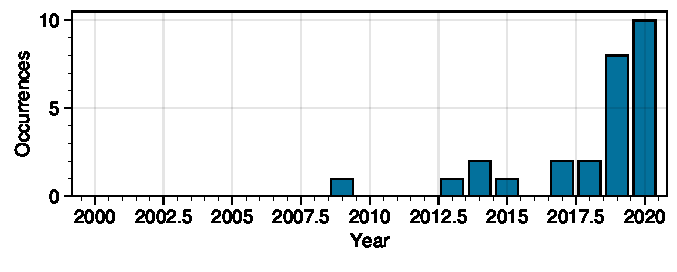
\includegraphics[width=8.3cm]{Figures/methods/Figure_4.pdf}
\caption{French alpine glaciers used for model training and validation and their classification into 3 clusters/regions (Écrins, Vanoise, Mont-Blanc). Coordinates of bottom left map corner: 44º32'N, 5º40'E, coordinates of the top right map corner: 46º08'N, 7º17'E.}
\label{methods:fig4}
\end{wrapfigure}

Glacier ice thickness data come from \citet{farinotti_consensus_2019}, hereafter F19, based on the Randolph Glacier Inventory v6.0 \citep[RGI,][]{consortium_randolph_2017}. The ice thickness values represent the latest consensus estimate, averaging an ensemble of different methods based on the principles of ice flow dynamics to invert the ice thickness from surface characteristics.

We also have ice thickness data acquired by diverse field methods \citep[seismic, ground penetrating radar or hot water drilling,][]{rabatel_estimation_2018} for four glaciers of the GLACIOCLIM observatory. We compared these in situ thickness data, with the simulated ice thicknesses from F19 (refer to Supplements for detailed information). Although differences can be found (locally up to 100\% in the worst cases), no systematic biases were found with respect to glacier local slope nor glacier altitude; therefore, no systematic correction was applied to the dataset. The simulated ice thicknesses for Saint-Sorlin (2 \(km^2\), mean altitude = 2920 m.a.s.l., Écrins cluster) and Mer de Glace (28 \(km^2\), mean altitude = 2890 m.a.s.l., Mont-Blanc cluster) glaciers are  satisfactorily modelled by F19. Mer de Glace's tongue presents local errors of about 50 m, peaking at 100 m (30\% error) around 2000-2100 m.a.s.l, but the overall distribution of the ice is well represented. Saint Sorlin glacier follows a similar pattern, with maximum errors of around 20 m (20\% error) at 2900 m.a.s.l. and a good representation of the ice distribution. The ice thicknesses for Argentière Glacier (12.8 \(km^2\), mean altitude = 2808 m.a.s.l., Mont-Blanc cluster) and Glacier Blanc (4.7 \(km^2\), mean altitude = 3196 m.a.s.l., Écrins cluster) are underestimated by F19 with an almost constant bias with respect to altitude, as seen in \citet{rabatel_estimation_2018}. Therefore, a manual correction was applied to the F19 datasets for these two glaciers based on the field observations from the GLACIOCLIM observatory. A detailed plot (Fig. \ref{methods:figS2}) presenting these results can be found in the supplementary material.

\subsubsection{Climate data}

In our French Alps case study, ALPGM is forced with daily mean near-surface (2 m) temperatures, daily cumulative snowfall and rain. The SAFRAN dataset is used to provide this data close to the glaciers’ centroids. SAFRAN meteorological data \citep{durand_reanalysis_2009} is a reanalysis of weather data including observations from different networks, and specific to the French mountain regions (Alps, Pyrenees and Corsica). Instead of being structured as a grid, data is provided at the scale of massifs, which are in turn divided into altitude bands of 300 meters and into 5 different aspects (north, south, east, west and flat). 

\subsection{Glacier-wide surface mass balance simulations: validation and results} \label{methods:case_study:SMB}

In this section, we go through the selection of SMB predictors, we introduce the procedure for building machine learning SMB models, we assess their performance in space and time and we show some results of simulations using the French alpine glaciers dataset. 

\subsubsection{Selection of predictors}

Statistical relationships between meteorological and topographical variables with respect to glacier-wide SMB are frequent in the literature for the European Alps \citep{hoinkes_glacier_1968}. \citet{martin_correlation_1974} performed a sensitivity study on the SMB of the Saint-Sorlin and Sarennes glaciers (French Alps) with respect to multi-annual meteorological observations for the 1957-1972 period. \citet{martin_correlation_1974} obtained a multiple linear regression function based on annual precipitation and summer temperatures, and he concluded that it could be further improved by differentiating winter and summer precipitations. \citet{six_sensitivity_2014} studied the sensitivity of the SMB to climate change in the French Alps from 1998 until 2014. They found that the variance of summer SMB is responsible for over 90\% of the variance of the annual glacier-wide SMB. \citet{rabatel_changes_2013, rabatel_spatio-temporal_2016} performed an extensive sensitivity analysis of different topographical variables (slope of the lowermost 20\% of the glacier area, mean elevation, surface area, length, minimum elevation, maximum elevation, surface area change and length change) with respect to glacier ELA and annual glacier-wide SMBs of French alpine glaciers. Together with \citet{huss_extrapolating_2012}, who performed a similar study with SMB, the most significant statistical relationships were found for the lowermost 20\% area slope, the mean elevation, glacier surface area, aspect and easting and northing. \citet{rabatel_changes_2013} also determined that the climatic interannual variability is mainly responsible for driving the glacier equilibrium-line altitude temporal variability, whereas the topographical characteristics are responsible for the spatial variations in the mean ELA. 

Summer ablation is often accounted for by means of cumulative positive degree days (CPDD). However, in the vast majority of studies, accumulation and ablation periods are defined between fixed dates (\textit{e.g.}, 1st October - 30th April for the accumulation period in the northern mid-latitudes) based on optimizations. As discussed in \citet{zekollari_statistical_2018}, these fixed periods may not be the best to describe SMB variability through statistical correlation. Moreover, the ablation season will likely evolve in the coming century, due to climate warming. In order to overcome these limitations, we dynamically calculate each year the transition between accumulation and ablation seasons (and vice-versa) based on a chosen quantile in the CPDD. We found higher correlations between annual SMB and ablation-period CPDD calculated using this dynamical ablation season. On the other hand, it was not the case for the separation between summer and winter snowfall. Therefore, we decided to keep constant periods to account for winter (1st October-1st May) and summer (1st May-1st October) snowfalls, and to keep them dynamical for the CPDD calculation.

Following this literature review, vectors $\hat{\Omega}$ and $\hat{C}$ from (Eq. \ref{eq:1}) read as:

\begin{equation} \label{eq:2}
\hat{\Omega}=\left[\begin{array}{lllllll}{\overline{Z}   \quad Z_{\max }   \quad \alpha_{20\%}  \quad \text {Area}  \quad \text{Lat}  \quad \text{Lon }  \quad \Phi }\end{array}\right]
\end{equation}

\begin{equation} \label{eq:3}
\widehat{C}=\left[\begin{array}{lllll}{\Delta C P D D} \quad {\Delta W S} \quad {\Delta S S} \quad {\Delta \overline{T}_{\operatorname{mon}}} \quad {\Delta \overline{S}_{\operatorname{mon}}}\end{array}\right]
\end{equation}
\\ 
Where: \\
$\overline{Z}$: Mean glacier altitude \\
$\quad Z_{\max }$: Maximum glacier altitude \\
$\quad \alpha_{20\%}$: Slope of the lowermost 20\% glacier altitudinal range \\
$Area$: Glacier surface area \\
$Lat$: Glacier latitude \\
$Lon$: Glacier longitude \\
$\Phi$: Cosine of the glacier’s aspect (North = 0º) \\
${\Delta C P D D}$: CPDD (Cumulative Positive Degree Days) anomaly \\
${\Delta W S}$: Winter snow anomaly \\
${\Delta S S}$: Summer snow anomaly \\
${\Delta \overline{T}_{\operatorname{mon}}}$: Average temperature anomaly for each month for the hydrological year \\
${\Delta \overline{S}_{\operatorname{mon}}}$: Average snowfall anomaly for each month for the hydrological year \\

For the linear machine learning models training, we chose a function $f$ that linearly combines $\hat{\Omega}$ and $\hat{C}$, generating new combined predictors (Eq. \ref{eq:4}). In $\hat{C}$, only ${\Delta CPDD}$, ${\Delta WS}$, and ${\Delta SS}$ are combined, to avoid generating an unnecessary amount of predictors with the combination of $\hat{\Omega}$ with ${\Delta \overline{T}_{\operatorname{mon}}}$ and ${\Delta \overline{S}_{\operatorname{mon}}}$.

\begin{equation} \label{eq:4}
\begin{flushleft}
\begin{math}
\begin{aligned}
S M B_{g, y} ={} & ((a_{1} \overline{Z}+a_{2} Z_{\max }+a_{3} \alpha_{20\%}+a_{4} Area+a_{5} Lat+a_{6} L o n+a_{7} \Phi+a_{8}) \Delta CPDD + \\
& (b_{1} \overline{Z}+b_{2} Z_{\max }+b_{3} \alpha_{20\%}+b_{4} Area+b_{5} L a t+b_{6} L o n+b_{7} \Phi+b_{8}) \Delta SS + \\
& (c_{1} \overline{Z}+c_{2} Z_{\max }+c_{3} \alpha_{20\%}+c_{4} Area+c_{5} Lat+c_{6} Lon+c_{7} \Phi+c_{8}) \Delta WS + \\
& d_{1} \overline{Z}+d_{2} Z_{\max }+d_{3} \alpha_{20\%}+d_{4} Area+d_{5} Lat+d_{6} Lon+d_{7} \Phi+d_{8} + d_{n}{\Delta \overline{T}_{\operatorname{mon}}} + d_{m}{\Delta \overline{S}_{\operatorname{mon}}} + \varepsilon )_{\text{g,y}}
\end{aligned}
\end{math}
\end{flushleft}
\end{equation}
\\
32 glaciers over variable periods between 31 and 57 years result in 1048 glacier-wide SMB ground truth values. For each glacier-wide SMB value, 55 predictors were produced following Eq. \ref{eq:4} 33 combined predictors, with ${\Delta \overline{T}_{\operatorname{mon}}}$ and ${\Delta \overline{S}_{\operatorname{mon}}}$ accounting for 12 predictors each, one for each month of the year. All these values combined produce a 1048x55 matrix, given as input data to the OLS and Lasso machine learning libraries. Early Lasso tests (not shown here) using only the predictors from Eq. \ref{eq:2} and \ref{eq:3} demonstrated the benefits of expanding the number of predictors, as it is later shown in Fig. \ref{methods:fig5}. For the training of the ANN, no combination of topo-climatic predictors is done as previously mentioned (Sect. \ref{methods:methods:SMB}), since it is already done internally by the ANN. 

\subsubsection{Causal analysis}

\begin{wrapfigure}{R}{0.55\linewidth}
\centering
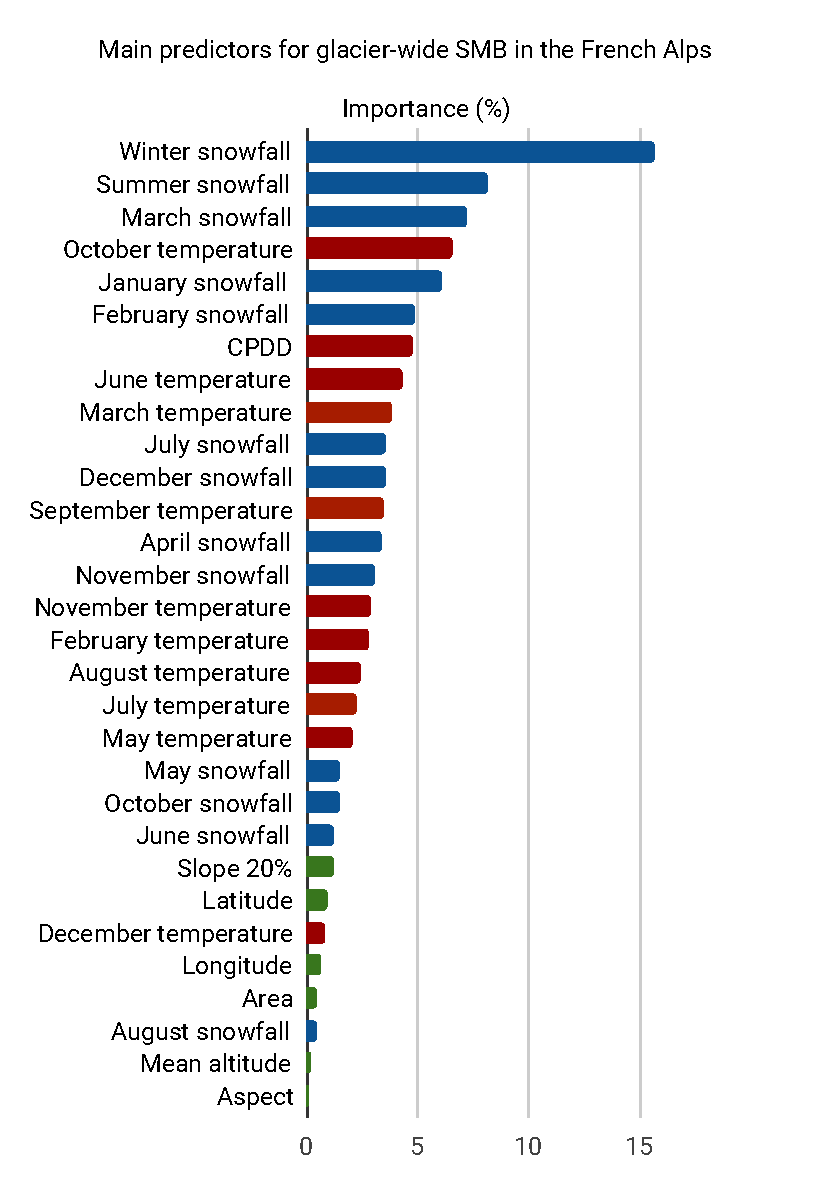
\includegraphics[width=8.3cm]{Figures/methods/Figure_5.pdf}
\caption{Contribution to the total variance of the 30 top topo-climatic predictors out of 55 predictors using Lasso. Green bars indicate predictors including topographical features, blue ones including accumulation-related features, and red ones including ablation-related features}
\label{methods:fig5}
\end{wrapfigure}

By running the Lasso algorithm on the dataset based on Eq. \ref{eq:2} and \ref{eq:3}, we obtain the contribution of each predictor in order to explain the annual glacier-wide SMB variance. Regarding the climatic variables, accumulation-related predictors (winter snowfall, summer snowfall as well as several winter, spring and even summer months), appear as the most important predictors. Ablation-related predictors also seem to be relevant, mainly with CPDD and summer and shoulder season months (Fig. \ref{methods:fig5}). Interestingly, meteorological conditions in the transition months are crucial for the annual glacier-wide SMB in the French Alps: (1) October temperature is determinant for the transition between the ablation and the accumulation season, favouring a lengthening of melting when temperature remains positive, or conversely allowing snowfalls that protect the ice and contribute to the accumulation when temperatures are negative; (2) March snowfall has a similar effect: positive anomalies contribute to the total accumulation at the glacier surface, and a thicker snow pack will delay the snow/ice transition during the ablation season leading to a less negative ablation rate \citep[e.g. Fig. \ref{methods:fig6}b,][]{reveillet_relative_2018}. Therefore, meteorological conditions of these transition months seem to strongly impact the annual glacier-wide SMB variability, since their variability oscillates between positive and negative values, unlike the months in the heart of summer or winter. 

In a second term, topographical predictors do play a role, albeit a secondary one. The slope of the 20\% lowermost altitudinal range, the glacier area, the glacier mean altitude and aspect help to modulate the glacier-wide SMB signal, which unlike point or altitude-dependent SMB, partially depends on glacier topography \citep{huss_conventional_2012}. Moreover, latitude and longitude are among the most relevant topographical predictors, which for this case study are likely to be used as bias correctors of precipitation of the SAFRAN climate reanalysis. SAFRAN is suspected of having a precipitation bias, with higher uncertainties for high altitude precipitations \citep{vionnet_numerical_2016}. Since the French Alps present an altitudinal gradient, with higher altitudes towards the eastern and the northern massifs, we found that the coefficients linked to latitude and longitude enhanced glacier-wide SMBs with a north-east gradient. 

\subsubsection{Spatial predictive analysis}

In order to evaluate the performance of the machine learning SMB models in space, we perform a leave-one-glacier-out (LOGO) cross-validation. For relatively small datasets like the one used in this study, cross-validation ensures that the model is validated on the full dataset. Such validation aims at understanding the model’s performance for predictions on other glaciers for the same time period as during the training. 

An important aspect is the comparison between linear and nonlinear machine learning algorithms used in this study. \citet{steiner_application_2005} already proved that a nonlinear ANN improved the results with respect a classic stepwise multiple linear regression. Here, we draw a similar comparison using more advanced methods for a larger dataset: OLS and Lasso as linear machine learning algorithms and a deep ANN as a nonlinear one. We observed significant differences between OLS, Lasso and deep learning, both in terms of explained variance (\(r^2\)) and accuracy (RMSE) of predicted glacier-wide SMBs. On average, we found improvements between +55\% and +61\% in the explained variance (from 0.49 to 0.76-0.79) using the nonlinear deep ANN compared to Lasso, whereas the accuracy was improved up to 45\% (from 0.74 to 0.51-0.62). This means that 27\% more variance is explained with a nonlinear model in the spatial dimension for glacier-wide SMB in this region (Fig. \ref{methods:fig6}). An interesting consequence of the nonlinearity of the ANN is the fact that it better captures extreme SMB values compared to a linear model. A linear model can correctly approximate the main cluster of values around the median, but the linear approximation performs poorly for extreme annual glacier-wide SMB values. The ANN solves this problem, with an increased explained variance which translates into a better accuracy for extreme SMB values, even without the use of sample weights (Fig. \ref{methods:fig6}). 

\begin{figure*}[t]
\centering
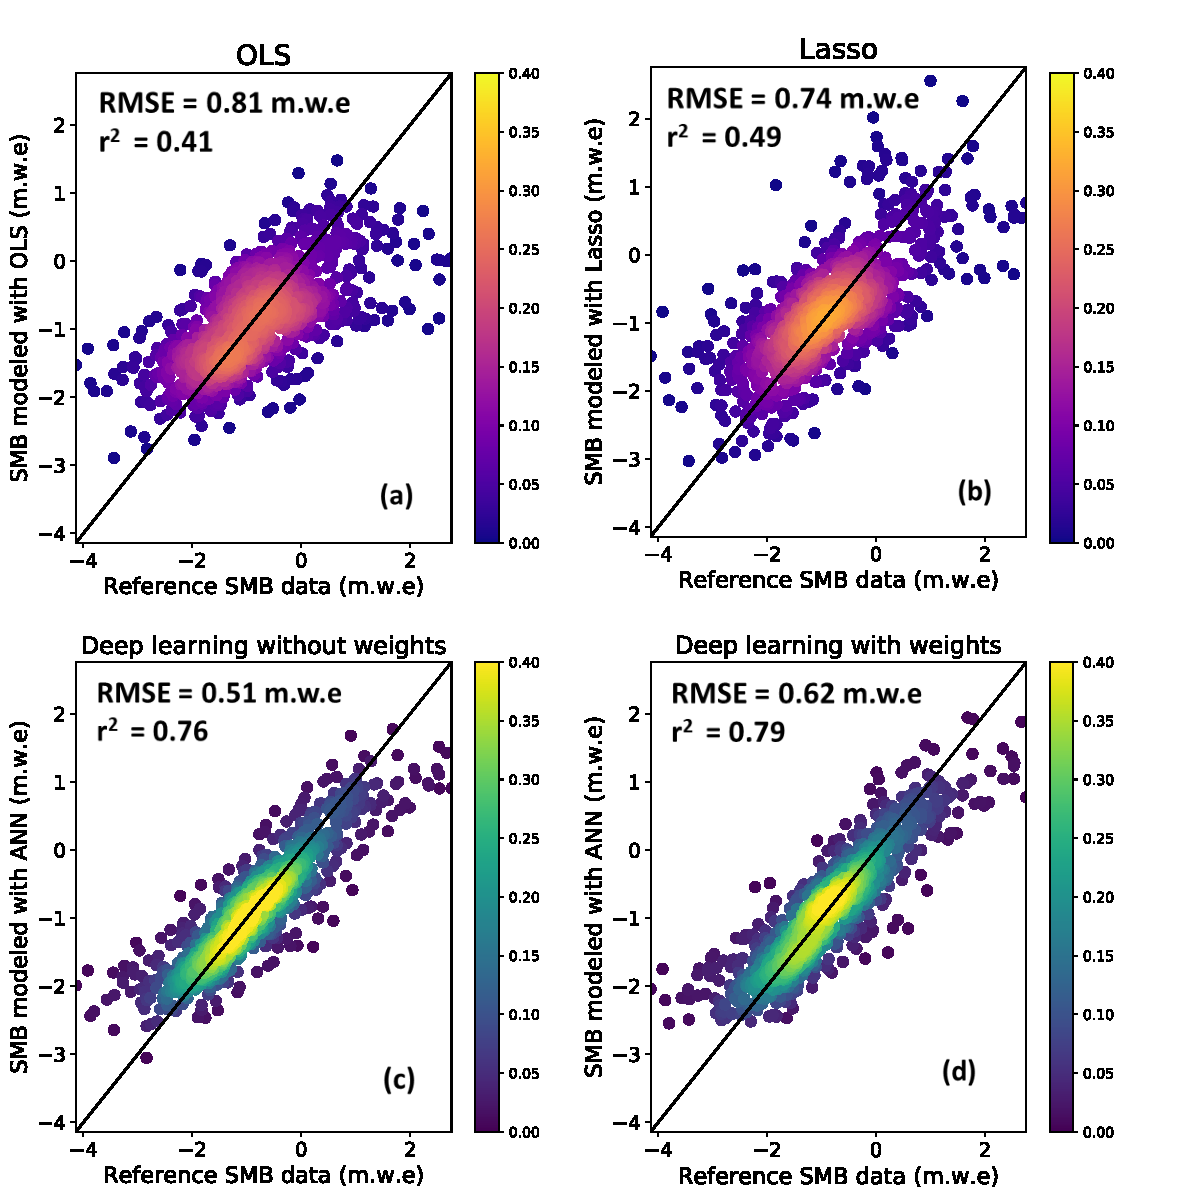
\includegraphics[width=12cm]{Figures/methods/Figure_6.pdf}
\caption{Evaluation of modelled annual glacier-wide SMB against the ground truth SMB data (both in m.w.e. $ a^{-1}$) using Leave-One-Glacier-Out cross-validation. The colour (purple-orange for linear; blue-green for nonlinear) indicates frequency based on the probability density function. The black line indicates the reference one-to-one line. a) Scatter plot of the OLS model results; b) Scatter plot of the Lasso linear model results; Scatter plots of the deep artificial neural network nonlinear models without (c) and with sample weights (d)}
\label{methods:fig6}
\end{figure*}

As a consequence, the added value of deep learning is especially relevant on glaciers with steeper annual changes in glacier-wide SMB (Fig. \ref{methods:fig7}a). The use of sample weights can scale up or down this factor, thus playing with a performance trade-off depending on how much one wants to improve the model’s behaviour for extreme SMB values. 

\begin{figure*}[t]
\centering
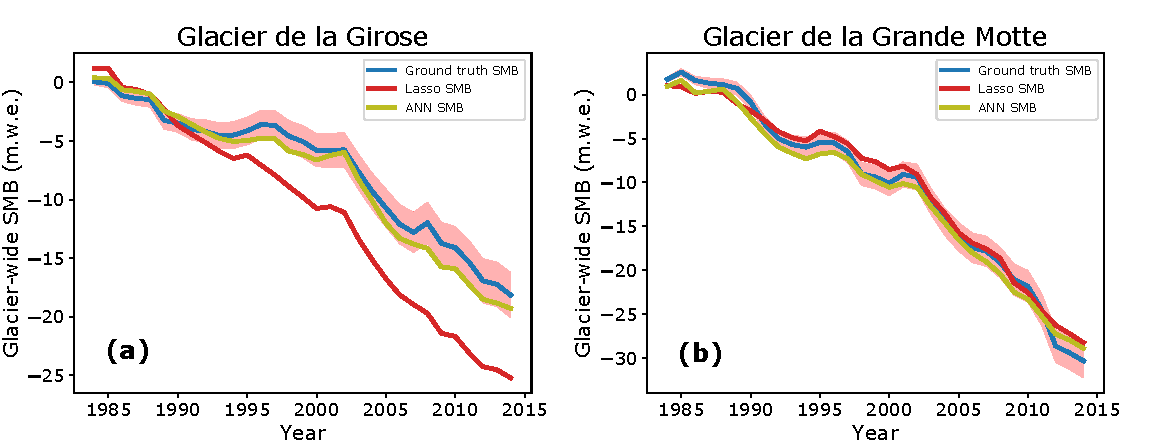
\includegraphics[width=14cm]{Figures/methods/Figure_7.pdf}
\caption{Examples of cumulative glacier-wide SMB (m.w.e.) simulations against the ground truth SMB data. The pink envelope indicates the accumulated uncertainties from the ground truth data. The deep learning SMB model has not been trained with sample weights in these illustrations.}
\label{methods:fig7}
\end{figure*}

Overall, deep learning results in a lower error throughout all the glaciers in the dataset when evaluated using LOGO cross-validation (Fig. \ref{methods:fig8}). Moreover, the bias is also systematically reduced, but it is strongly correlated to the one from Lasso. 

\begin{figure*}[t]
\centering
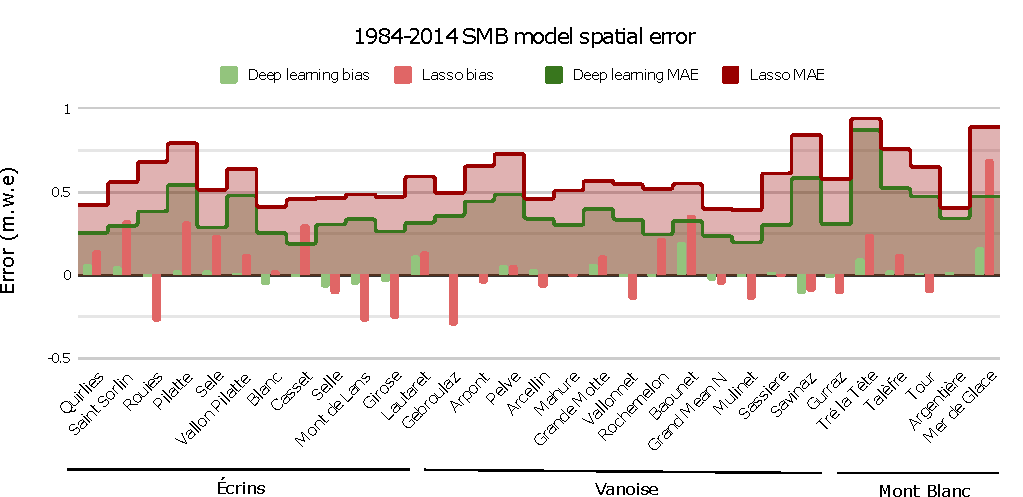
\includegraphics[width=16cm]{Figures/methods/Figure_8.pdf}
\caption{Mean average error (MAE) and bias (vertical bars) for each glacier of the training dataset structured by clusters for the 1984-2014 LOGO glacier-wide SMB simulation. No clear regional error patterns arise}
\label{methods:fig8}
\end{figure*}

\subsubsection{Temporal predictive analysis}

In order to evaluate the performance of the machine learning SMB models in time, we perform a leave-one-year-out (LOYO) cross-validation. This validation serves to understand the model’s performance for past or future periods outside the training time period. The best results achieved for Lasso make no use of any monthly average temperature or snowfall, suggesting that these features are not relevant for temporal predictions unlike the spatial case.

As in Sect. \ref{methods:case_study:SMB}, the results between the linear and nonlinear machine learning algorithms were compared. Interestingly, using LOYO, the differences between the different models were even greater than for spatial validation, revealing the more complex nature of the information in the temporal dimension. As illustrated by Fig. \ref{methods:fig9}, we found remarkable improvements between the linear Lasso and the nonlinear deep learning in both the explained variance (between +94\% and +108\%) and accuracy (between +32\% and +58\%). This implies that 35\% more variance is explained using a nonlinear model in the temporal dimension for glacier-wide SMB balance in this region. Deep learning manages to keep very similar performances between the spatial and temporal dimensions, whereas the linear methods see their performance affected most likely due to the increased nonlinearity of the SMB reaction to meteorological conditions. 

\begin{figure*}[h]
\centering
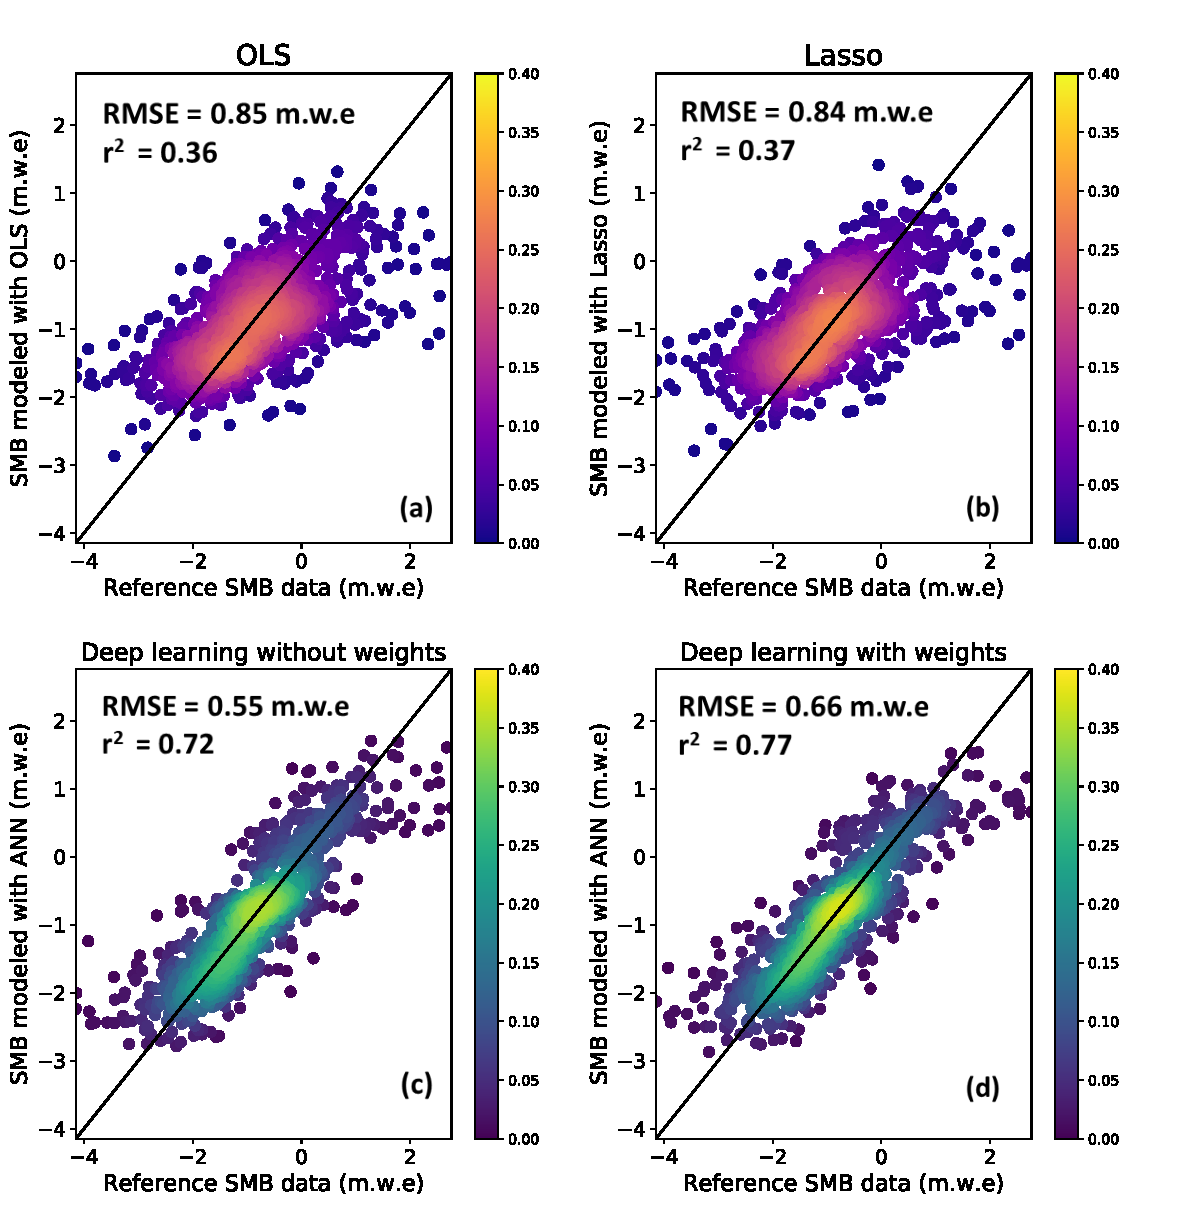
\includegraphics[width=12cm]{Figures/methods/Figure_9.pdf}
\caption{Evaluation of modelled annual glacier-wide SMB against the ground truth SMB data (both in m.w.e. $ a^{-1}$) using Leave-One-Year-Out cross-validation. The colour (purple-orange for linear; blue-green for nonlinear) indicates frequency based on the probability density function. The black line indicates the reference one-to-one line. a) Scatter plot of the OLS model results; b) Scatter plot of the Lasso linear model results; Scatter plots of the deep artificial neural network nonlinear models without (c) and with sample weights (d).}
\label{methods:fig9}
\end{figure*}

A more detailed year by year analysis reveals interesting information about the glacier-wide SMB data structure. As seen in Fig. \ref{methods:fig10}, the years with the worst deep learning precision are 1984, 1985 and 1990. All these three hydrological years present a high spatial variability in observed (or remotely-sensed) SMBs: very positive SMB values in general for 1984 and 1985 with few slightly negative values, and extremely negative SMB values in general for 1990 with few almost neutral values. These complex configurations are clearly outliers within the dataset, which push the limits of the nonlinear patterns found by the ANN. The situation becomes even more evident with Lasso, which struggles to resolve these complex patterns and often performs poorly where the ANN succeeds (\textit{e.g.}, years 1996, 2012 or 2014). The important bias present only with Lasso is representative of its lack of complexity towards nonlinear structures, which results in an underfitting of the data. The average error is not bad, but it shows a high negative bias for the first half of the period, which mostly has slightly negative glacier-wide SMBs, and a high positive bias for the second half of the period, which mostly has very negative glacier-wide SMB values.

\begin{figure*}[t]
\centering
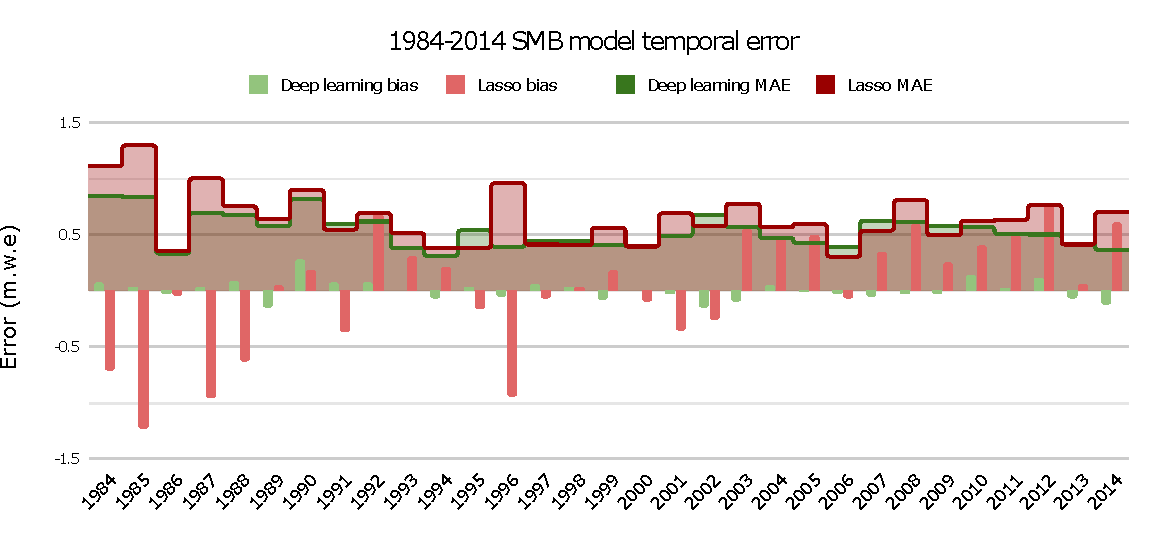
\includegraphics[width=16cm]{Figures/methods/Figure_10.pdf}
\caption{Mean average error (MAE) and bias (vertical bars) for each year of the training dataset for the 1984-2014 LOYO glacier-wide SMB simulation.}
\label{methods:fig10}
\end{figure*}

\subsubsection{Spatiotemporal predictive analysis}

Once the specific performances in the spatial and temporal dimensions have been assessed, the performance in both dimensions at the same time is evaluated using Leave-Some-Years-and-Glaciers-Out (LSYGO) cross-validation. 64 folds were built, with test folds being comprised of data for 2 random glaciers on 2 random years, and train folds of all the data except the 2 years (for all glaciers) and the 2 glaciers (for all years) present in the test fold. These combinations are quite strict, implying that for every 4 tested values we need to drop between 123 and 126 values for training, depending on the glacier and year, to respect the spatiotemporal independence \citep{roberts_cross-validation_2017}. 

The performance of LSYGO is similar to LOYO, with a RMSE of 0.51 m.w.e. and a coefficient of determination of 0.77 (Fig. \ref{methods:figS5}).  This is reflected in the fact that very similar ANN hyperparameters were used for the training. This means that the deep learning SMB model is successful in generalizing and it does not overfit the training data. 

\subsection{Glacier geometry evolution: Validation and results} 
\label{methods:case_study:deltah}

As mentioned in Sect. \ref{methods:methods:deltah}, the Δh parameterization has been widely used in many studies \citep[e.g.,][]{huss_modelling_2008, huss_future_2010, vincent_future_2014, huss_new_2015, huss_global-scale_2018, hanzer_projected_2018, vincent_declin_2019}. It is not in the scope of this study to evaluate the performance of this method, but we present the approach developed in ALPGM to compute the $\Delta$h functions and show some examples for single glaciers to illustrate how these glacier-specific functions perform compared to observations. For the studied French alpine glaciers, the 1979-2011 period is used. This period was proved by \citet{vincent_future_2014} to be representative of Mer de Glace’s secular trend. Other sub-periods could have been used, but it was shown that they did not necessarily improve the performance. In addition, the 1979 and 2011 DEMs are the only ones available that cover all the French alpine glaciers. Within this period, some years with neutral to even positive surface mass balances in the late 1970s and early 1980s can be found, as well as a remarkable change from 2003 onward with strongly negative surface mass balances, following the heatwave that severely affected the western Alps in summer 2003.

The glacier-specific $\Delta$h functions are computed for glaciers $\geq$ 0.5 \(km^2\), which represented about 80\% of the whole glaciarized surface of the French Alps in 2015 (some examples are illustrated in the Supplement Fig. \ref{methods:figS4}). For the rest of very small glaciers (< 0.5 \(km^2\)), a standardized flat function is used in order to make them shrink equally at all altitudes. This is done to simulate the fact that generally, the equilibrium line of very small glaciers has surpassed the glacier’s maximum altitude, thus shrinking from all directions and altitudes in summer. Moreover, due to their reduced size and altitudinal range, the ice flow no longer has the same importance as for larger or medium sized glaciers.

In order to evaluate the performance of the parameterized glacier dynamics of ALPGM, coupled with the glacier-wide SMB component, we compared the simulated glacier area of the 32 studied glaciers with the observed area in 2015 from the most up-to-date glacier inventory in the French Alps. Simulations were started in 2003, for which we used the F19 ice thickness dataset. In order to take into account the ice thickness uncertainties, we ran three simulations with different versions of the initial ice thickness: the original data, -30\% and +30\% of the original ice thickness in agreement with the uncertainty estimated by the authors. Moreover, in order to take into account the uncertainties in the $\Delta$h glacier geometry update function computation, we added a ±10\% variation in the parameterized functions (Fig. \ref{methods:fig11}).

\begin{figure*}[h]
\centering
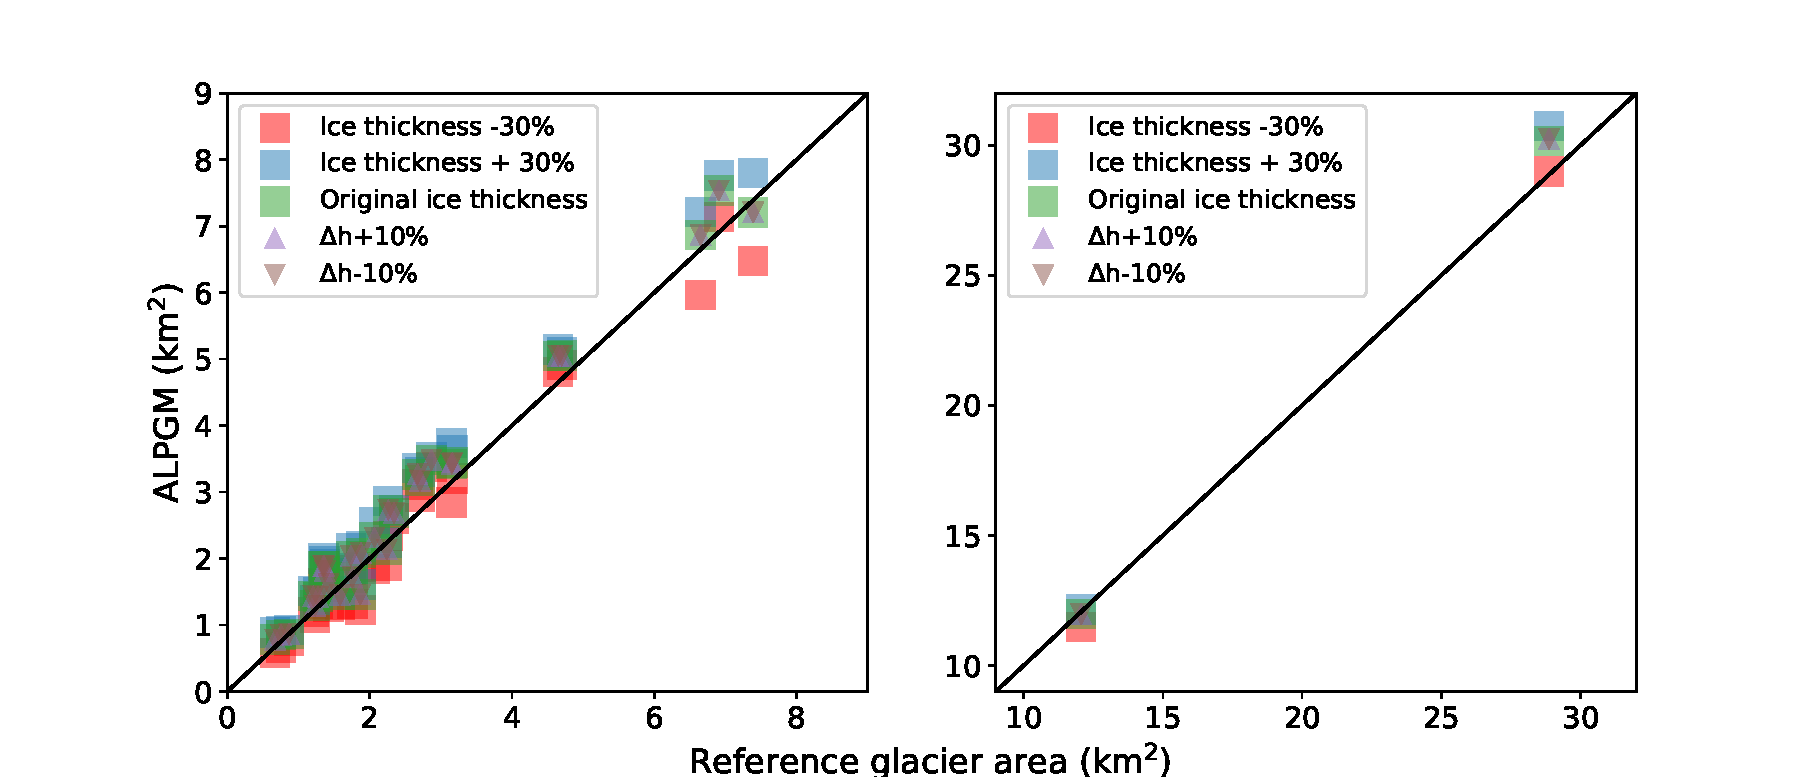
\includegraphics[width=15cm]{Figures/methods/Figure_11.pdf}
\caption{Simulated glacier areas for the 2003-2015 period for the 32 study glaciers using a deep learning SMB model without weights. Squares indicate the different F19 initial ice thicknesses used taking into account their uncertainties and triangles indicate the uncertainties linked to the glacier-specific geometry update functions. For better visualisation, the figure is split in two with the two largest French glaciers on the right.}
\label{methods:fig11}
\end{figure*}

Overall, the results illustrated in Fig. \ref{methods:fig11} show a good agreement with the observations. Even for a 12-year period, the initial ice thickness remains the largest uncertainty, with almost all glaciers falling within the observed area when taking it into account. The mean error in simulated surface area was of 10.7\% with the original F19 ice thickness dataset. Other studies using the $\Delta$h parameterization already proved that the initial ice thickness is the most important uncertainty in glacier evolution simulations, together with the choice of a GCM for future projections \citep{huss_new_2015}. 

\section{Discussion and perspectives} \label{methods:discussion}

\subsection{Linear methods still matter} \label{methods:discussion:linear}

Despite the fact that deep learning often outperforms linear machine learning and statistical methods, there is still a place for such methods in modelling. Indeed, unlike ANNs, simpler regularised linear models such as Lasso allow an easy interpretation of the coefficients associated to each input feature, which helps to understand the contribution of each of the chosen variables to the model. This means that linear machine learning methods can be used for both prediction and causal analysis. Training a linear model in parallel to an ANN has therefore the advantage to provide a simpler linear alternative which can be used to understand the dataset. Moreover, seeing the contribution of each coefficient, one can reduce the complexity of the dataset by keeping only the most significant predictors. Finally, a linear model serves as well as a reference to highlight and quantify the nonlinear gains obtained by deep learning. 

\subsection{Training deep learning models with spatiotemporal data} \label{methods:spatiotemporal}

The creation and training of a deep ANN requires a certain knowledge and strategy with respect to the data and study focus. When working with spatiotemporal data, the separation between training and validation becomes tricky. The spatial and temporal dimensions in the dataset cannot be ignored, and strongly affect the independence between training and validation data \citep{roberts_cross-validation_2017, berlingerio_evaluation_2019}. Depending on how the cross-validation is performed, the obtained performance will be indicative of one of these two dimensions. As it is shown in Sect. \ref{methods:case_study:SMB}, the ANNs and especially the linear modelling approaches had more success in predicting SMB values in space than in time. This is mostly due to the fact that the glacier-wide SMB signal has a greater variability and nonlinearities in time than in space, with climate being the main driver of the annual fluctuations in SMB, whereas geography, and in particular the local topography, modulates the signal between glaciers \citep{huss_extrapolating_2012, rabatel_spatio-temporal_2016, vincent_common_2017}. Consequently, linear models find it easier to make predictions on a given period of time for other glaciers elsewhere in space, than for time periods outside the training. Nonetheless, the deep learning SMB models were capable of equally capturing the complex nonlinear patterns in both the spatial and temporal dimensions. 

In order to cope with the specific challenges related to each type of cross-validation, there are several hyperparameters that can be modified to adapt the ANN’s behaviour. Due to the long list of hyperparameters intervening in an ANN, it is not advisable to select them using brute force with a grid search or cross-validation. Instead, initial tests are performed in a subset of random folds to narrow down the range of best performing values, before moving to the full final cross-validations for the final hyperparameter selection. Moreover, the ANN architecture plays an important role: the number of neurons as well as the number of hidden layers will determine the ANN’s complexity and its capabilities to capture hidden patterns in the data. But the larger the architecture, the higher are the chances to overfit the data. This undesired effect can be counterbalanced using regularization. The amount of regularization (dropout and Gaussian noise in our case, see Sect. \ref{methods:methods:SMB}) used in the training of the ANN necessarily introduces some trade-offs. The greater the dropout, the more we will constrain the learning of the ANN so the higher the generalization will be, until a certain point, where relevant information will start to be lost and performance will drop. On the other hand, the learning rate to compute the stochastic gradient descent, which tries to minimize the loss function, also plays an important role: smaller learning rates generally result in a slower convergence towards the absolute minima, thus producing models with better generalization. By balancing all these different effects, one can achieve the accuracy versus generalization ratio that best suits a certain dataset and model in terms of performance. Nonetheless, one key aspect in machine learning models is data: expanding the training dataset in the future will allow to increase the complexity of the model and its performance. Consequently, machine learning models see their performance improved as time goes by, with new data becoming available for training. 

Although the features used as input for the model are classical descriptors of the topographical and meteorological conditions of the glaciers, it is worth mentioning that applying the model in different areas or with different data sources would likely require a re-training of the model due to possible biases: different regions on the globe may have other descriptors of importance but also different measuring techniques will likely have different biases. 

\subsection{Perspectives on future applications of deep learning in glaciology} \label{methods:deeplearning}

The currently used meteorological variables in the deep ANN of ALPGM’s SMB component are based on the classic degree-day approach, which relies only on temperature and precipitation. However, the model could be trained with variables involved in more complex models, such as SEB-type models, for which the longwave and shortwave radiation, as well as the turbulent fluxes and albedo intervene. The current model framework allows flexibility in the choice and number of input variables that can reflect different degrees of complexity for the resolved processes. Despite the fact that it has been shown that for glaciers in the European Alps there is almost no added value in transitioning from a simple degree-day to a SEB model for annual glacier-wide SMB simulations \cite[e.g.,][]{reveillet_which_2017}, it could be an interesting way to expand the training dataset for glaciers in tropical and subtropical regions, where shortwave radiation plays a much more important role \citep{benn_glaciers_2014}. \citet{maussion_enso_2015} followed a similar approach with linear machine learning in order to calibrate a regression-based downscaling model that linked local SEB/SMB fluxes to atmospheric reanalysis variables. 

In this work, we also evaluated the resilience of the deep learning approach: since many glacierized regions in the world do not have the same amount of data used in this study, we trained an ANN only with monthly average temperature and snowfall, without any topographical predictors, to see until which point the algorithm is capable of learning from minimal data. The results were quite interesting, with a coefficient of determination of 0.68 (against 0.76 from the full model) and a RMSE of 0.59 m.w.e. $a^-1$ (against 0.51 from the full model). These results indicate that meteorological data is the primary source of information, determining the interannual high frequency variability of the glacier-wide SMB signal. On the other hand, the “bonus” of topographical data helps to  modulate the high frequency climate signal, by adding a low frequency component to better differentiate glaciers and the topographical characteristics included in the glacier-wide SMB data \citep{huss_conventional_2012}. The fact that glacier-wide SMB is influenced by glacier topography poses the question of determining if the simulated glacier geometries can correctly reproduce topographical observations, needed to represent the topographical feedback present in glacier-wide SMB signals. These aspects are analyzed and discussed in Sect. \ref{methods:case_study} of the Supplementary material, showing small differences between the observed and simulated topographical parameters for the 2003-2015 period (Table S1). Additionally, the simulated glacier-wide SMBs using simulated topographical parameters show very small differences (0.069 m.w.e. $a^-1$ on average) compared to simulations using topographical observations (Fig. \ref{methods:figS6}). Since glacier ice thickness estimates date from the year 2003 \citep{farinotti_consensus_2019}, our validation period can only encompass 12 years. According to all the available data for validation, our model seems to be able to correctly reproduce the glacier geometry evolution, but since the 2003-2015 validation period is quite short, the validation performance might not be representative when dealing with future glacier evolution projections of several decades. Consequently, these aspects will have to be taken into account for future studies using this modelling approach for projections. Moreover, the cross-validation results of the SMB model(s) (Fig. \ref{methods:fig6}-\ref{methods:fig10}) are representative of the performance of predictions using topographical observations. Despite the small differences found between simulated and observed topographical parameters, the SMB model's performance might be slightly different than the performance found in the cross-validation analysis. Therefore, it would be interesting for future studies to investigate the use of point SMB data, which could avoid the complexities related to the influence of glacier topography in glacier-wide SMB. 

A nonlinear deep learning SMB component like the one used for ALPGM could provide an interesting alternative to classical SMB models used for regional modelling. The comparison with other SMB models is beyond the scope of this study, but it would be worth investigating to quantify the specific gains that could be achieved by switching to a deep learning modelling approach. Nonetheless, the linear machine learning models trained with the CPDD and cumulative snowfall used in this study behave in a similar way to a calibrated temperature-index model. Even so, we believe that future efforts should be taken towards physics-informed data science glacier SMB and evolution modelling. Adding physical constraints in ANNs, with the use of physics-based loss functions and/or architectures \cite[e.g.,][]{karpatne_physics-guided_2018}, would allow to improve our understanding and confidence in predictions, reduce our dependency on big datasets, and to start bridging the gap between data science and physical methods \citep{karpatne_theory-guided_2017, de_bezenac_deep_2018, lguensat_learning_2019, rackauckas_universal_2020}.  Deep learning can be of special interest once applied in the reconstruction of SMB time series. More and more SMB data is becoming available thanks to the advances in remote sensing \citep[e.g.,][]{brun_spatially_2017, zemp_global_2019, dussaillant_two_2019}, but these datasets often cover limited areas and the most recent time period in the studied regions. An interesting way of expanding a dataset would be to use a deep learning approach to fill the data gaps, based on the relationships found in a subset of glaciers as in the case study presented here. Past SMB time series of vast glaciarized regions could thereby be reconstructed, with potential applications in remote glaciarized regions such as the Andes or High Mountain Asia. 

\section{Conclusions} 

We presented a novel approach to simulate and reconstruct glacier-wide SMB series using deep learning for individual glaciers at a regional scale. This method has been included as a SMB component in ALPGM \citep{bolibar_jordibolibar/alpgm:_2019}, a parameterized regional glacier evolution model, following an alternative approach to most physical and process-based glacier models. The data-driven glacier-wide SMB modelling component is coupled with a glacier geometry update component, based on glacier-specific parameterized functions. Deep learning is shown to outperform linear methods for the simulation of glacier-wide SMB with a case study of French alpine glaciers. By means of cross-validation, we demonstrated how important nonlinear structures (up to 35\%) coming from the glacier and climate systems in both the spatial and temporal dimensions are captured by the deep ANN. Taking into account this nonlinearity substantially improved the explained variance and accuracy compared to linear statistical models, especially in the more complex temporal dimension. As we have shown in our case study, deep ANNs are capable of dealing with relatively small datasets, and they present a wide range of configurations to generalize and prevent overfitting. Machine learning models benefit from the increasing number of available data, which makes their performance constantly improve as time goes by. 

Deep learning should be seen as an opportunity by the glaciology community. Its good performance for SMB modelling in both the spatial and temporal dimensions shows how relevant it can be for a broad range of applications. Combined with in situ or remote sensing SMB estimations, it can serve to reconstruct SMB time series for regions or glaciers with already available data for past and future periods, with potential applications in remote regions such as the Andes or the high mountains of Asia. Moreover, deep learning can be used as an alternative to classical SMB models as it is done in ALPGM: important nonlinearities from the glacier and climate systems are potentially ignored by these mostly linear models, which could give an advantage to deep learning models in regional studies. It might still be too early for the development of such models in certain regions which lack consistent datasets with a good spatial and temporal coverage. Nevertheless, upcoming methods adding physical knowledge to constrain neural networks \cite[e.g.,][]{karpatne_physics-guided_2018, rackauckas_universal_2020} could provide interesting solutions to the limitations of our current method. By incorporating prior physical knowledge in neural networks, the dependency on big datasets would be reduced, and it would allow to transition towards more interpretable physics-informed data science models. 

\section{Supplementary material}

\subsection{Filtering of DEM rasters}

Before computing the glacier-specific $\Delta$h parameterized functions, some preprocessing is done to the regional French Alps DEM raster files in order to filter artefacts and noise. The processing chain works as follows:

\begin{enumerate}
 
\item The regional DEM files are cropped using the 2003 glacier inventory shapefile outlines, thus obtaining glacier-specific rasters with the DEMs from 1979 and 2011.
\item The glacier surface altitude difference for this period (so-called dh/dt) which corresponds to the change in ice thickness is computed glacier by glacier by subtracting the two previously mentioned DEM rasters.
\item A first empirical filter is applied to all rasters to filter unrealistic values coming from artefacts (e.g., presence of clouds or saturation on the images used to generate de DEMs).
\item The filtered ice thickness difference (dh/dt) and DEM rasters are paired together as in Figure 12, and a low-order polynomial fit is applied in order to get the main trend of the scatterplot between the ice thickness difference vs. altitude.
\item A dynamic envelope/buffer around the polynomial fit line is computed for each glacier based on a quantile between maximum and minimum values for each altitude. In order to smooth the computed envelope for each altitude, a convolutional filter is applied to these values in order to smooth them and to follow the polynomial fit. A dynamic sliding window size is used to adjust the averaging process to the characteristics of each glacier. 
\item A second filter is then applied using the computed smoothed envelope buffer to remove outliers
\item A final polynomial fit is computed with a variable order depending on the number of remaining data values of each glacier.
\item The percentage of pixels of information available for computing the polynomial fit (the parameterized function) is displayed for each glacier at the end of the processing chain.

\end{enumerate}
 
\subsection{SMB statistical error analysis}

In order to determine the error due to each predictor, a Lasso model was trained with the same training matrix as the ANN, but instead of using SMB as ground truth data the errors generated by the ANN without weights were used. As discussed in section \ref{methods:discussion:linear}, Lasso performs a regularization on the training dataset, thus keeping only certain predictors and removing the rest. By looking at the resulting coefficients of the model, we can estimate the linear contribution of each predictor to the final model error. Latitude and longitude appear as the most important error predictors, but their contribution might in fact indicate the different magnitude of errors between glaciers or regions, since the pair of coordinates specifically identifies each glacier. October, August and March temperature follow behind, indicating that changes in temperature during these months have an influence in the simulation errors. It is not surprising that two of these months appear as top predictors (Fig. \ref{methods:fig5}), as changes in temperature during these months at the transition between the accumulation and ablation season can have a strong importance on the surface mass balance processes. 

\begin{figure*}[h]
\centering
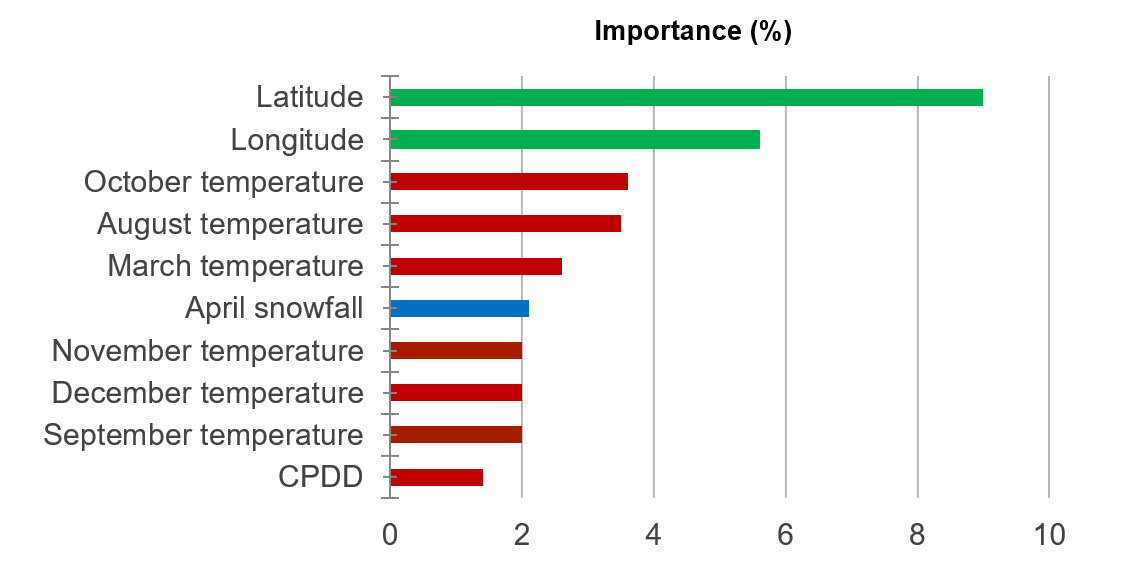
\includegraphics[width=12cm]{Figures/methods/Figure_S1.png}
\caption{Importance (\%) of the first 10 predictors using Lasso to predict residual error from the ANN SMB model. Green bars indicate topographical features, red bars temperature-related features and blue bars precipitation-related features.}
\label{methods:figS1}
\end{figure*}

Such an approach to analyze the influence of the different predictors into the quantification of uncertainties is of course limited, since a linear model is trained with nonlinear results. But these results are useful to determine the main contributors to errors rather than quantifying these errors, which has been done with the LOGO, LOYO and LSYGO cross-validations. 

\subsection{Topographical glacier-wide SMB predictors}

Since topography plays a role in the glacier-wide SMB signal, besides the climate, the representation of the glacier’s topography is important in order to correctly simulate its glacier-wide SMB and its geometrical evolution. As explained in Sect. \ref{methods:methods} “Model overview and workflow” and Sect. \ref{methods:case_study:data} “Topographical glacier data and altimetry”, the source of the topographical predictors used for the simulation of glacier-wide SMB is different at different steps of the glacier evolution simulation chain. Two cases exist:

\begin{enumerate}
 
\item For the machine learning training of the glacier-wide SMB models, which is performed on historical data, all topographical data comes from the multitemporal glacier inventories (Gardent et al., 2014, with 2015 update). In order to have an annual timestep, topographical data from these inventories are linearly interpolated. 
\item For the full glacier evolution simulation, coupling the glacier-wide SMB component with the glacier geometry evolution component, the model must be capable of generating all the input topographical predictors even for non-observed glaciers and future periods. For every glacier and year, all the topographical predictors are computed from the updated glacier-specific ice thickness and DEM raster files from Farinotti et al. (2019), which then are used to simulate a single glacier-wide SMB for that glacier and year. Then, this glacier-wide SMB together with the glacier-specific geometry update function are used to update the glacier’s geometry and their respective ice thickness and DEM rasters. For the next year, all the topographical predictors are recomputed with the updated raster files, and this process is repeated in a loop with an annual timestep. Therefore, the glacier-wide SMB model is called with an annual timestep, simulating only single values in order to take into account the evolution of the glacier’s topography. 

\end{enumerate}

In order to show that the glacier geometry update component, coupled with the glacier-wide SMB simulation component can successfully simulate the evolution of the topographical characteristics of glaciers in the region, a specific test was designed. Using the same validation period as in Sect. \ref{methods:case_study:SMB} (2003-2015), we ran parallel simulations of glacier-wide SMB for all the 32 case study glaciers. The first simulation was done using case (1), with the multitemporal glacier inventories data, and the second one was done following case (2), with the full glacier evolution model and the Farinotti et al. (2019) raster files. The results of both simulations were really similar, revealing only small differences. On average, the simulated glacier-wide SMBs for this period differed on 0.069 m.w.e. a$^{-1}$, due to the differences in the input topographical predictors, which are computed from different datasets (Fig. \ref{methods:figS6}). Moreover, the performances of both simulations for this period are very similar, with a RMSE of 0.49 m.w.e. a$^{-1}$ for case (1) and 0.52 m.w.e. a$^{-1}$ for case (2). The results with all the differences between the simulated glacier-wide SMB values and input topographical values are summarized in Table \ref{methods:tableS1}:

\\

\begin{table}[h!]
\centering
\begin{tabular}{ | m{4cm} | m{2.5cm}| m{1.5cm} | m{4cm} | m{1cm} |} 
 \hline
 Variable (multitemporal inventories vs. full glacier    evolution) & SMB simulated & Slope & Average glacier elevation & Area\\
 \hline MAE or mean difference  & 0.069 m.w.e a$^{-1}$	  & 1.8º	 & 31.3 m & 0.2 km$^{2}$ \\
\hline
\end{tabular}
\caption{Differences on simulated glacier-wide SMB and topographical predictors between a simulation using interpolated topographical predictors from the multitemporal glacier inventories and the full glacier evolution simulations including the coupling of the glacier-wide SMB with the glacier geometry update. }
\label{methods:tableS1}
\end{table}

\\

The only striking difference is perhaps the difference in simulated areas. This is mainly due to the fact that the Farinotti et al. (2019) dataset uses the RGI v6, which for the largest glaciers of Argentière and Mer de Glace, overestimates its surface area (from 32 to 34 km2 for Mer de Glace in 2003). The differences in slope are explained by the fact that this variable is not included in the multitemporal glacier inventories (Gardent et al., 2014), therefore it has been computed once with a global DEM and kept constant for each glacier throughout the years for the training of the SMB model. On the other hand, in order to include the long term effects of glacier morphology changes in the glacier evolution simulations (glacier-wide SMB simulation + glacier geometry update), the glacier slope is re-computed with an annual timestep and it evolves through time. Therefore, there are small differences for certain glaciers whose slope has evolved during this period, thus accounting for the differences with the fixed value used for the training of the SMB model.
 
This test serves to prove that the full glacier evolution simulations in ALPGM are capable of reproducing the topographical predictors used for the training of the glacier-wide SMB machine learning models. Moreover, this test also helps to prove that ALPGM can correctly simulate the topographical evolution of glaciers, which allows to capture the topography induced feedback, which plays a role in the simulation of glacier-wide SMBs. 

\subsection{Supplementary figures}

\begin{figure*}[h]
\centering
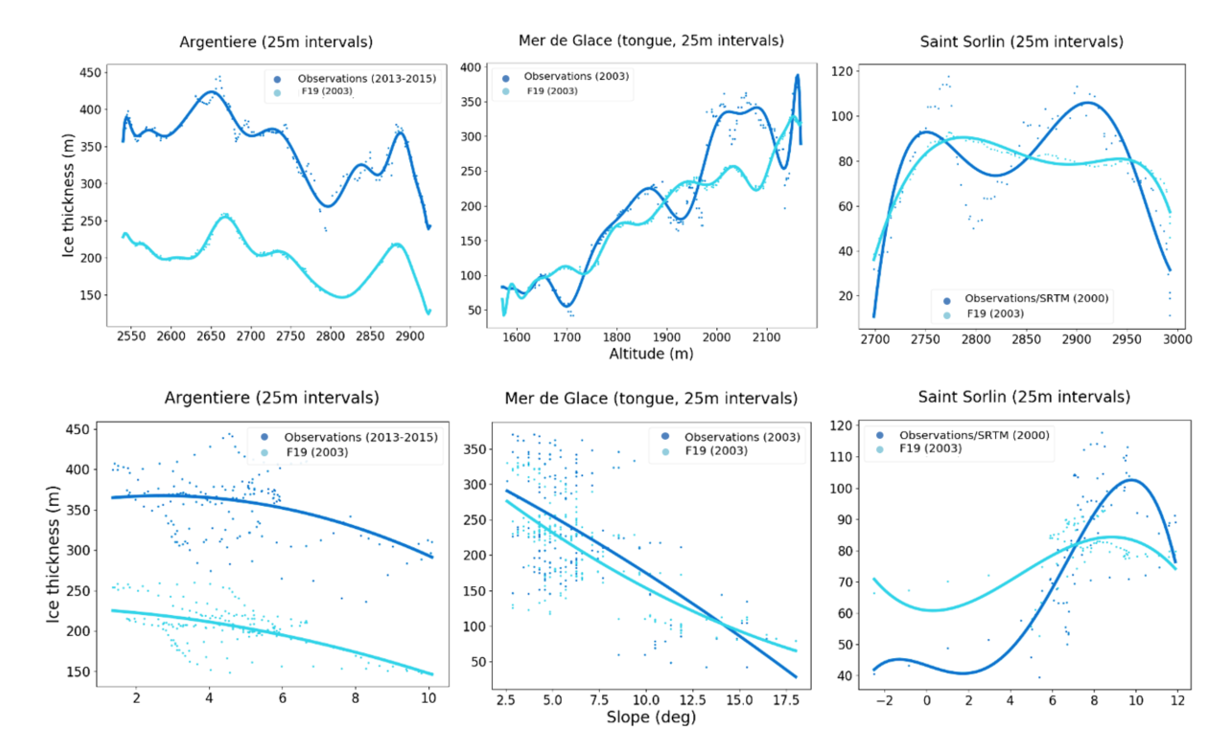
\includegraphics[width=15cm]{Figures/methods/Figure_S2.png}
\caption{Comparison of simulated glacier ice thicknesses from F19 with observations from the GLACIOCLIM observatory. Points are compared at 25 m intervals on the glacier flowline. The polynomial fits have less degrees of freedom for the slope plots. Note that for some glaciers the dates are not the same}
\label{methods:figS2}
\end{figure*}

\begin{figure*}[h]
\centering
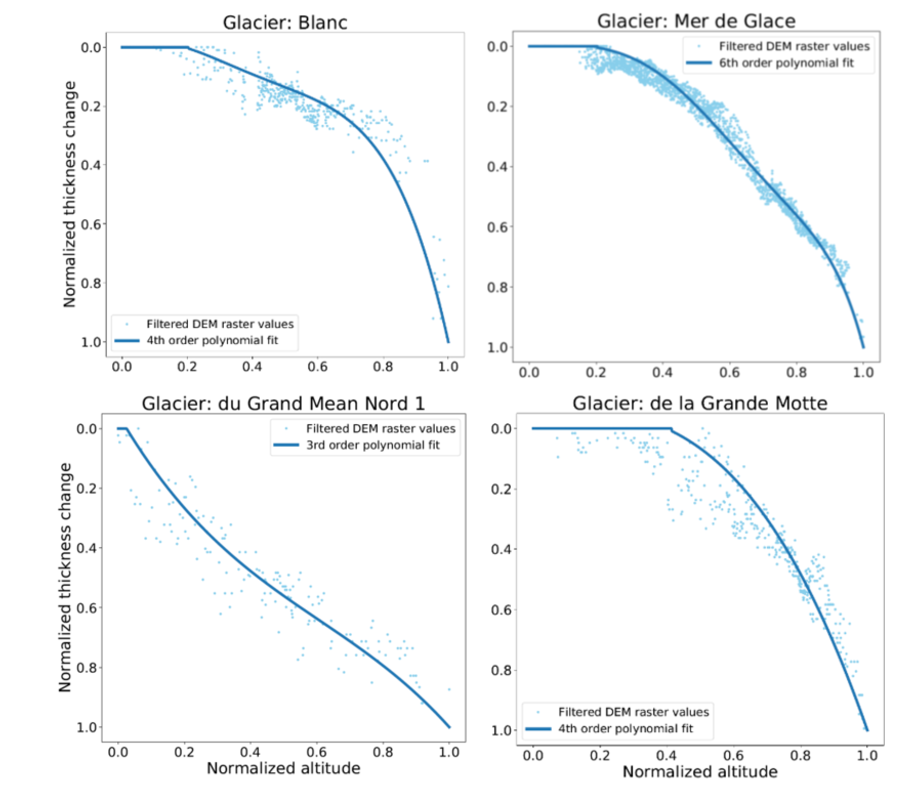
\includegraphics[width=14cm]{Figures/methods/Figure_S3.png}
\caption{Examples of glacier specific $\Delta$h parameterized functions generated by ALPGM. The order of the polynomial fit depends on the number of available pixels.}
\end{figure*}

\begin{figure*}[h]
\centering
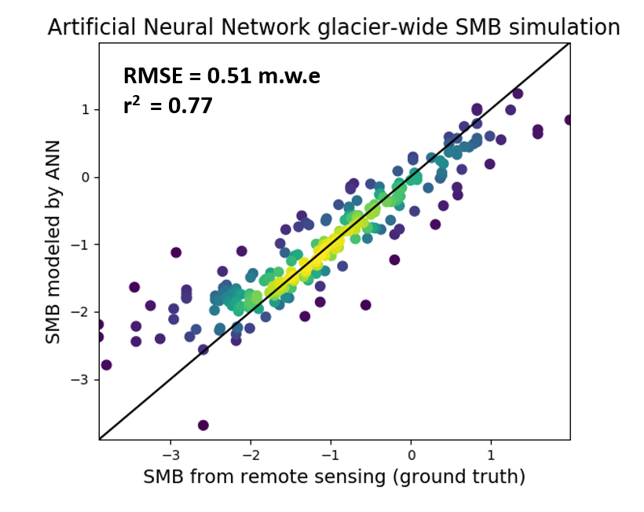
\includegraphics[width=9cm]{Figures/methods/Figure_S4.png}
\caption{Results for the spatiotemporal cross-validation using Leave-Some-Glaciers-and-Years-Out (LSYGO). SMB values are in m.w.e. Compared to the other scatter plots from 3.2, there are less values available for test due to the severity of the spatiotemporal independence.}
\label{methods:figS4}
\end{figure*}

\begin{figure*}[h]
\centering
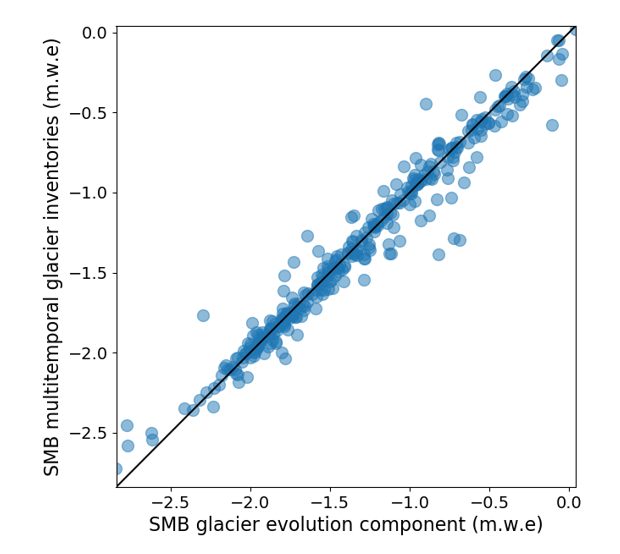
\includegraphics[width=9cm]{Figures/methods/Figure_S5.png}
\caption{Comparison of glacier-wide SMB simulations (2003-2015, 32 case study glaciers) using topographical predictors from the multitemporal glacier inventories (Y axis) vs. using the full glacier evolution simulations in ALPGM with the Farinotti et al. (2019) ice thickness and DEM rasters (X axis). Average difference = 0.069 m.w.e.  a$^{-1}$}
\label{methods:figS5}
\end{figure*}

\begin{figure*}[h]
\centering
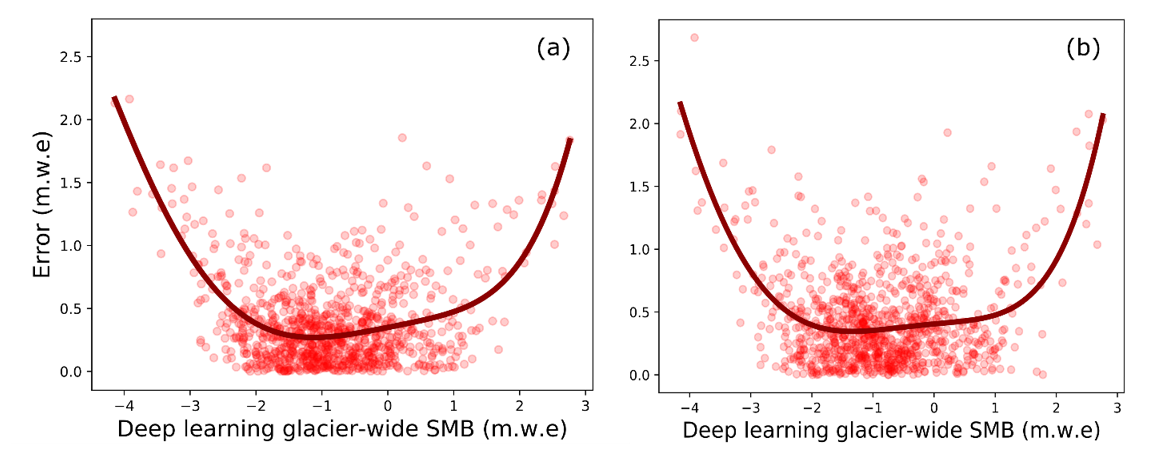
\includegraphics[width=15cm]{Figures/methods/Figure_S6.png}
\caption{Error distribution of deep learning (without weights) glacier-wide SMB simulations for the 1984-2015 period for the 32 case study glaciers. (a) Performance in the spatial dimension using LOGO cross-validation; (b) performance in the temporal dimension using LOYO cross-validation. The red line corresponds to a 5th order polynomial fit.}
\label{methods:figS6}
\end{figure*}
 



\chapter{A deep learning reconstruction of mass balance series for all glaciers in the French Alps: 1967-2015}
\label{chap:past}

\begin{flushright}
{\small \textit{In using the present in order to reveal the past, we assume that the forces in the world are essentially the same through all time; for these forces are based on the very nature of matter.}\\
James Dwight Dana}
\end{flushright}

\section*{Preface}

After the development of the deep learning modelling approach, it was clear that the initial objectives of this PhD project regarding the glacio-hydrological modelling of the Rhône catchment would be transformed. In order to properly apply this new method to a regional-scale scientific problem, we decided to use all climate, topographical and glaciological data available during the last 50 years in the French Alps, in order to reconstruct annual mass balance series for all French alpine glaciers. This new study, served as a proof of concept of the methodology, but also enabled the presentation of a new open reference dataset of mass balance changes in the French Alps. Despite the high quality and availability of data for this region and period, as it always happens in science, inference is based on hypotheses. Empirical and statistical approaches can suffer when applied to largely different conditions, proving wrong the words of James Dwight Dana. Following the philosophy of the previous chapter, we tried again to be as sure as possible that we were obtaining the results for the right reasons. This dataset carries indeed important uncertainties, particularly for very small glaciers, but it represents, to our knowledge, the best approximation on how the mass balance of French alpine glaciers evolved through the last half century. I am very grateful for the reviews by Ben Marzeion and Matthias Huss during the open peer review of this paper. I cannot think of more qualified people to judge my work, and I was greatly pleased with their constructive and thoughtful comments, that helped to improve this study in many ways. A common thread throughout this PhD work has been to render this work as transparent and open as possible. By sharing the source-code used for simulations, and publishing the results in open-access journals and repositories, I aim at doing my part to make science a more accessible and transparent collective enterprise. 

\textit{Based on Bolibar, J., Rabatel, A., Gouttevin, I. and Galiez, C.: A deep learning reconstruction of mass balance series for all glaciers in the French Alps: 1967-2015, Earth System Science Data, preprint, Cryosphere – Glaciology., 2020.}


\section{Abstract}

Glacier mass balance (MB) data are crucial to understand and quantify the regional effects of climate on glaciers and the high-mountain water cycle, yet observations cover only a small fraction of glaciers in the world. We present a dataset of annual glacier-wide mass balance of all the glaciers in the French Alps for the 1967-2015 period. This dataset has been reconstructed using deep learning (i.e. a deep artificial neural network), based on direct MB observations and remote sensing annual estimates, meteorological reanalyses and topographical data from glacier inventories. The method's validity was assessed previously through an extensive cross-validation against a dataset of 32 glaciers , with an estimated average error (RMSE) of 0.55 m.w.e. a$^{-1}$,  an explained variance ($r^{2}$) of 75\% and an average bias of -0.021 m.w.e. a$^{-1}$. We estimate an average regional area-weighted glacier-wide MB of -0.69±0.21 (1$\sigma$) m.w.e. a$^{-1}$ for the 1967-2015 period, with negative mass balances in the 1970s (-0.44 m.w.e. a$^{-1}$), moderately negative in the 1980s (-0.16 m.w.e. a$^{-1}$), and an increasing negative trend from the 1990s onwards, up to -1.26 m.w.e. a$^{-1}$ in the 2010s. Following a topographical and regional analysis, we estimate that the massifs with the highest mass losses for the 1967-2015 period are the Chablais (-0.93 m.w.e. a$^{-1}$), Champsaur (-0.86 m.w.e. a$^{-1}$) and  Haute-Maurienne and Ubaye ranges (-0.84 m.w.e. a$^{-1}$ both), and the ones presenting the lowest mass losses are the Mont-Blanc (-0.68 m.w.e. a$^{-1}$), Oisans and Haute-Tarentaise ranges (-0.75 m.w.e. a$^{-1}$ both). This dataset - available at: https://doi.org/10.5281/zenodo.3925378
 \citep{bolibar_deep_2020} - provides relevant and timely data for studies in the fields of glaciology, hydrology and ecology in the French Alps, in need of regional or glacier-specific annual net glacier mass changes in glacierized catchments.
 
\section{Introduction}

Among all the components of the Earth system, glaciers are some of the most visibly affected by climate change, with an overall worldwide shrinkage despite important differences between regions (Zemp et al., 2019). The European Alps are among the regions with the strongest glacier mass loss over recent decades, with expected mass losses between 60\% and 95\% by the end of the 21st century \citep{zekollari_modelling_2019}. These major glacier mass changes are likely to have an impact on water resources, society and alpine ecosystems \citep[e.g.][]{huss_global-scale_2018, immerzeel_importance_2020, cauvy-fraunie_global_2019}. In order to study and quantify all these potential consequences, the availability of glacier mass balance data is of high relevance. Therefore, open historical datasets are crucial for the understanding of the driving processes and the calibration of models used for projections. Unlike glacier length, glacier mass balance (MB) provides a more direct indicator of the climate-glacier interactions \citep{marzeion_past_2012}. Glacier surface mass balance (SMB) is classically measured using the direct or glaciological method, by separately determining the ablation and accumulation totals. Direct measurements quantify the surface mass balance at different points of the glacier, and these values must be integrated at the glacier scale in order to assess the glacier-wide SMB \citep{benn_glaciers_2014}. These different point SMB measurements can show a high nonlinear variability, which can complicate this integration process towards glacier-wide estimates \citep{vincent_nonlinear_2018}. Moreover, field measurements require a lot of manpower, time and economic resources in order to be sustained for a meaningful period of time. On the other hand, recent advances in remote sensing allow estimating glacier MB changes at a regional level with unprecedented efficiency using geodetic and gravimetric methods \citep{kaab_contrasting_2012, fischer_surface_2015, berthier_decadal_2016, brun_spatially_2017, dussaillant_two_2019}. Due to constraints related to the availability of digital elevation models (DEMs) or airborne data, these mass balance estimates normally encompass several years or decades. Some studies are bridging the gap towards an annual temporal resolution \citep{rabatel_using_2005, rabatel_spatio-temporal_2016, rastner_automated_2019}, but the coverage is still limited to glaciers without cloud cover or acquisition-related artefacts. This means that these mass balance datasets are often restricted to certain glaciers and years within a region. All these new datasets are extremely beneficial for data-driven approaches, fostering the training of machine learning models capable of capturing the regional characteristics and relationships \citep{bolibar_deep_2020-1}. This type of approach allows to fill the spatiotemporal gaps in the MB datasets, therefore, it can be seen as a complement to remote sensing and direct observations. 

On the other hand, MB reconstructions have already been carried out in the European Alps, providing a basis for comparison between different approaches (see \citet{hock_glaciermip_2019} for a compilation). Two studies include reconstructions in the European Alps, including the French Alps, over a substantial period of the recent past: \citet{marzeion_past_2012, marzeion_brief_2015} reconstructed annual MB series of all glaciers in the Randolph Glacier Inventory for the last century. They used a minimal model relying only on temperature and precipitation data, based on a temperature-index method, with two parameters to calibrate the temperature sensitivity and the precipitation lapse rate. \citet{huss_extrapolating_2012} presented an approach to extrapolate SMB series of a limited number of glaciers to the mountain-range scale. By comparing multiple methods, he found the best results with a multiple linear regression based on 6 topographical parameters. From this relationship he reconstructed area-averaged SMB series of all the glaciers of the European Alps between 1900-2100 and analysed the trends for the different alpine nations and different glacier sizes.

Here, we introduce a dataset of annual glacier-wide MB of all the glaciers in the French Alps \citep{bolibar_deep_2020}, located in the westernmost part of the European Alps, between 5.08° and 7.67°E, and 44° and 46°13’N. Glacier-wide MBs have been reconstructed for the 1967-2015 period, using deep learning (i.e. a deep artificial neural network) (Fig. \ref{past:fig1}). This approach was introduced in \citet{bolibar_deep_2020-1}, for which a deep artificial neural network (ANN) was trained with data from 32 French alpine glaciers, as part of the ALpine Parametrized Glacier Model (ALPGM) \citep{bolibar_alpgm_2020}. Annual glacier-wide MB values are reported for each glacier in the French Alps found in the 2003 glacier inventory \citep{gardent_multitemporal_2014}. An overview of the methodology used to produce the dataset and a review of the associated uncertainties is presented in Sect. \ref{past:methods}, followed by a dataset overview in Sect. \ref{past:overview}, where the data structure and regional trends are described and where the dataset is compared to a previous study and observations. 

\begin{figure}[t]
\centering
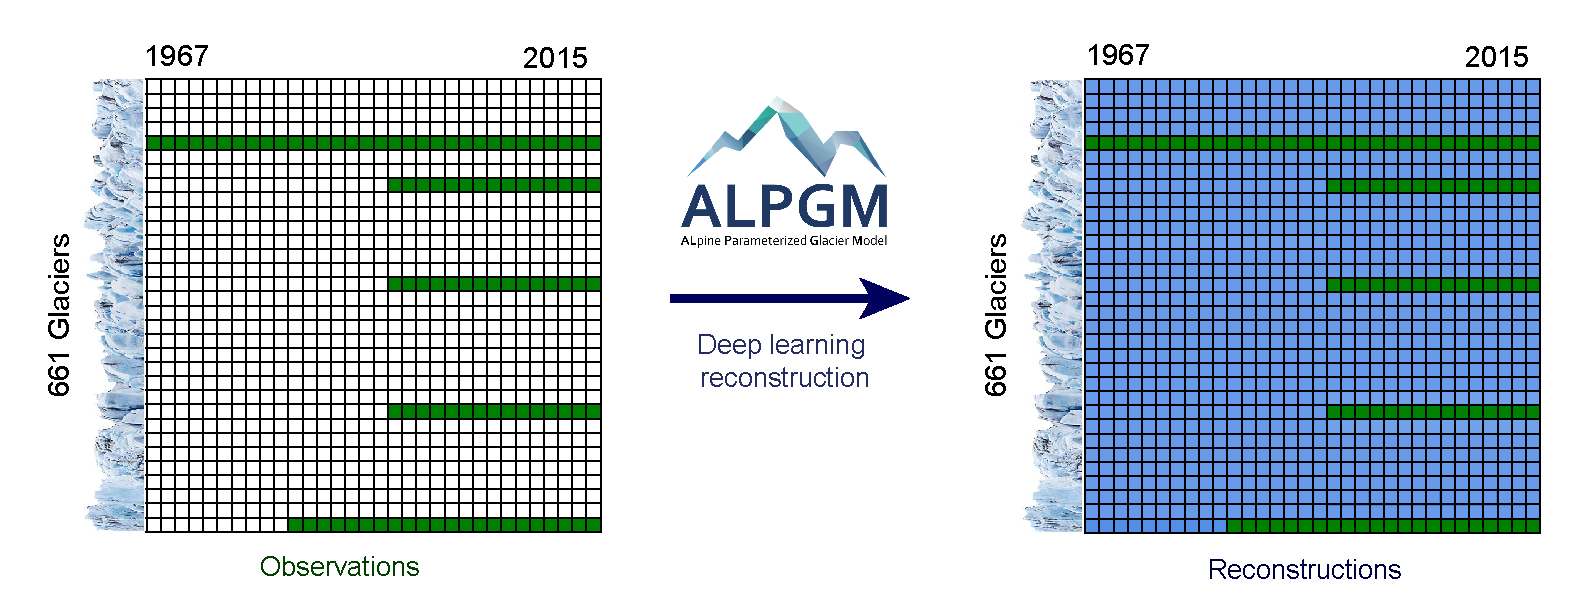
\includegraphics[width=15cm]{Figures/past/Figure_1.pdf}
\captionsetup{justification=centering}
\caption{Summary of the deep learning regional MB reconstruction approach. From the available annual glacier-wide MB data, a deep learning model is used to reconstruct the full dataset, thus filling the spatiotemporal gaps in the observational dataset. Green indicates glaciers and years with MB observations and remote sensing estimates, and blue indicates reconstructed MB values. Glacier ice cliffs in the vertical axis indicate rows representing individual glaciers. The grid size with glaciers and years is schematic and only serves to illustrate the concept.}
\label{past:fig1}
\end{figure}


\section{Data and methods} \label{past:methods}

\subsection{Training data} \label{past:methods:data}

For the reconstruction presented here, a dataset of 32 French alpine glaciers has been used for training, covering most of the massifs within the French Alps, which exhibit a great variability of topographical characteristics (Fig. \ref{past:figS10)}. The French Alps are located in the westernmost part of the European Alps, rising from the Mediterranean sea northwards between 44 and 46º13' N, 5.08 and 7.67º E. Due to its particular geographical setup, glacierized mountain ranges in the French Alps have distinct climatic signatures. Southern glaciers exhibit a Mediterranean influence, whereas northern glaciers are mostly affected by western fluxes from the Atlantic, except for eastern glaciers close to the Italian border, which are more influenced by east returns. 

Out of the 32 glaciers from this dataset, four glaciers include direct MB measurements from the GLACIOCLIM observatory, some of which since 1949. These direct observations have been calibrated using photogrammetric geodetic MB \citep{vincent_common_2017}. On the other hand, 28 glaciers include estimates of annual glacier-wide MB from remote sensing between 1984 and 2014 \citep{rabatel_spatio-temporal_2016}. These remote sensing estimates were computed using (1) the end-of-summer snowline for every year, which in the European Alps is a proxy of the equilibrium-line altitude (ELA); and (2) geodetic MB for the 1984-2014 period quantified from two high-resolution DEMs. Both data sources are used to reconstruct the annual glacier-wide MB of each individual glacier for the same period of the geodetic MB. 

This dataset of 32 glaciers, with a total of 1048 annual glacier-wide MB values, is used as a reference. Unlike point MB, glacier-wide MB is influenced by both climate and glacier geometry, producing complex interactions between climate and glacier morphology that  need to be taken into account in the model. For each annual glacier-wide MB value available, the following data are compiled to train the ANN with an annual time step: (1) climate data from the SAFRAN meteorological reanalyses \citep{durand_reanalysis_2009}, with: cumulative positive degree days (CPDD), cumulative winter snowfall, cumulative summer snowfall, mean monthly temperature and mean monthly snowfall, all variables being quantified at the altitude of the glacier's centroid. In order to capture the climate signal at each glacier's centroid, temperatures are taken from the nearest SAFRAN 300 m altitudinal band and adjusted with a 6 ºC/km lapse rate. The updated temperature is then used to update the rain-snow parts from the same 300 m altitudinal band. Snowfall is considered as all precipitation fallen at temperatures equal or lower than 0º C. (2) annually interpolated topographical data between the 1967, 1985, 2003 and 2015 glacier inventories in the French Alps \citep[update of][]{gardent_multitemporal_2014}, with: mean and maximum glacier altitude, slope of the lowermost 20\% altitudinal range of the glacier, surface area, latitude, longitude and aspect. Therefore, the topographical feedback of the shrinking glaciers is captured from these annually interpolated topographical predictors. These topoclimatic parameters were identified as relevant for glacier-wide MB modelling in the French Alps \citep{bolibar_deep_2020-1}, and the dates of the glacier inventories determined the time interval for the reconstructions presented here.

For more details on the choice of predictors, the reader can find a more detailed analysis in \citet{bolibar_deep_2020-1}.

\subsection{Methods} \label{past:methods:methods}

The annual glacier-wide MB dataset for the 661 French alpine glaciers has been reconstructed using a deep artificial neural network (ANN), also known as deep learning. ANNs are nonlinear statistical models inspired by biological neural networks \citep{fausett_fundamentals_1994, hastie_elements_2009}. Recent developments in the field of machine learning and optimization enabled the use of deeper ANN architectures, which allows capturing more nonlinear and complex patterns in data even for small datasets \citep{ingrassia_neural_2005}.  This modelling approach is part of the MB component of ALPGM \citep{bolibar_alpgm_2020}, an open-source data-driven parameterized glacier evolution model. For a detailed explanation of the methodology, please refer to \citet{bolibar_deep_2020-1}. For the final reconstructions presented here, a cross-validation ensemble approach was used based on 60 Leave-Some-Years-and-Glaciers-Out (LSYGO) cross-validation models. Individual predictions of each of the  members were averaged to produce a single output. An ensemble approach has the advantage of further improving generalization, and reducing overfitting as well as the inter-model high variance typical from neural networks \citep{krogh_neural_1995}. A weighted bagging approach \citep{hastie_elements_2009} was used in order to balance the dataset, giving more weight to under-represented data samples from the years 1967-1983. On the other hand, for the 32 glaciers with glacier-wide MB observations and remote sensing estimates used for training, an ensemble of 50 models trained with the full dataset was used, in order to achieve the best possible performance for this subset of glaciers, which represents a substantial fraction (45\% in 2003) of the total glacierized surface area in the French Alps.

\subsection{Uncertainty assessment} \label{past:methods:uncertainty}

The uncertainties linked to the deep learning approach used in this study have been assessed through cross-validation, for which deep learning predictions were compared with observations and remote sensing estimates. A detailed presentation of the method's uncertainties and performance from the cross-validation study can be found in \citet{bolibar_deep_2020-1}. Block cross-validation ensured that all the 32 glaciers in the dataset were evaluated, with spatiotemporal structures formed by glaciers and years being considered in order to prevent the violation of the assumption of independence \citep{roberts_cross-validation_2017}. This means that three different deep ANNs were produced: one for reconstructing glacier-wide MB in space, one for the reconstruction in time (future and past), and another one for both dimensions at the same time; each of these with a different calibration and performance. It was shown that the deep ANN performs better in the spatial dimension, in which the MB signal relationships with the predictors are the simplest. MB annual variability is mostly driven by climate, whereas geography and local topography (i.e. differences between glaciers) modulate the signal in space in a simpler way \citep{vincent_common_2017, bolibar_deep_2020-1}. Therefore, deep learning is capable of finding more structures in the spatial dimension, accounting for a better accuracy and explained variance compared to the temporal dimension. The deep ANN used in this study presents an RMSE of 0.55 m.w.e a$^{-1}$ with an $r^{2}$ of 0.75 in LSYGO cross validation. The ANN MB reconstructions accurately reproduce the annual variability of glaciological observations from the GLACIOCLIM observatory (Figure S1). This reinforces the trust in the produced model ensemble, indicating that models trained with  heterogeneous data comprised by glaciological and remote sensing estimates can correctly reproduce direct annual observations.  

\begin{figure}[t]
\centering
\includegraphics[width=11cm]{Figures/past/Figure_2.pdf}
\captionsetup{justification=centering}
\caption{Comparison of average annual glacier-wide MB for the 2000-2015 period between the glaciological MB from the GLACIOCLIM observatory (GC), the ASTER-derived geodetic MB from Davaze et al., 2020 (D20), the MB reconstructions from this study (B20) and the reconstructions from this study recalibrated using the ASTER-derived geodetic MB (B20').}
\label{past:fig2}
\end{figure}

Nonetheless, only one glacier in the training dataset is smaller than 0.5 km$^{2}$ (Glacier de Sarennes, 0.3 km$^{2}$ in 2003), implying that uncertainties for very small glaciers (< 0.5 km$^{2}$) might differ from those estimated using cross-validation. In 2015, very small glaciers in the French Alps represented about 80\% of the total glacier number, but they accounted for only 20\% of the total glacierized area. This means that their importance is relative, for example in terms of water resources, but a user of this dataset should bear in mind that MB from these very small glaciers might carry greater uncertainties than the ones assessed during cross-validation. This might be especially true for extremely small glaciers (< 0.05 km$^{2}$) which can be considered as spatial outliers for the deep ANN. Since there is only one glacier with MB observations for very small glaciers and none for extremely small glaciers, there is no precise way to quantify these uncertainties. On the other hand, the ANN is mostly trained with glacier-wide MB data between 1984 and 2014, with a reduced amount of values between 1967 and 1984 (986 and 62 values, respectively). Since this early period contains on average more positive and neutral glacier-wide MB values than the 1984-2014 period, the performance of the ANN was specifically assessed for this period. An additional cross-validation was performed with four folds, each with a glacier including glacier-wide MB data before 1984. For each fold, all MB data of that glacier and time period were hidden from the ANN, and the simulated glacier-wide MBs between 1967 and 1983 were tested in order to assess the model’s performance. The results showed that the ANN is capable of correctly reconstructing glacier-wide MB for glaciers and years before 1984 (Fig. \ref{past:figS5}), with an estimated accuracy (RMSE) of 0.47 m.w.e. a$^{-1}$ and an estimated explained variance ($r^{2}$) of  0.65. This uncertainty assessment is based on roughly 10\% of the full dataset, meaning that these estimates lack the robustness of the full cross-validation from \citet{bolibar_deep_2020-1}, but they serve to show that the model can accurately reconstruct glacier-wide MB data outside the main cluster of years used during training. 

In order to further validate the reconstructions presented here, a comparison against independent ASTER \citep{davaze_region-wide_2020} and Pléiades \citep{berthier_glacier_2014} geodetic MB data was performed, that helps to assess the bias of the MB reconstructions for the 2000-2015 (Fig. \ref{past:fig2}) and 2003-2012 (Fig. \ref{past:figS2}) sub-periods.  The photogrammetric geodetic MB used to calibrate the MB datasets from \citet{rabatel_spatio-temporal_2016} and the glaciological observations from GLACIOCLIM have a much higher resolution than ASTER-derived geodetic MB, but the comparison can bring interesting information for glaciers outside the training dataset. Our reconstructions show a good agreement with the geodetic MB for certain regions (e.g. Grandes Rousses), except for some particular steep large high-altitude glaciers (e.g. Bossons and Taconnaz in the Mont-Blanc massif) that substantially differ from most glaciers in the French Alps. A more detailed analysis and additional figures comparing the MB datasets can be found in Sect. \ref{past:supp:comparison} of the Supplementary. In order to exploit this additional geodetic MB dataset, we have recalibrated our MB reconstructions for the 2000-2015 period using the ASTER-derived geodetic MB from \citet{davaze_region-wide_2020} for some glaciers outside our training dataset (i.e. B20' in Fig. \ref{past:fig2}). Since ASTER-derived geodetic MB present important uncertainties for small glaciers (i.e. < 1 km$^{2}$), we have only recalibrated MB series for 16 large glaciers outside the training dataset with uncertainties lower than 0.15 m.w.e. a$^{-1}$. The calibration has been performed by adding the average annual bias between \citet{davaze_region-wide_2020} and this study for the 2000-2015 sub-period.


\section{Dataset overview} \label{past:overview}

\subsection{Dataset format and content} \label{past:overview:format}

The MB dataset is presented in two different formats: (a) A single netCDF file containing the MB reconstructions, the glacier RGI and GLIMS IDs and the glacier names. This file contains all the necessary information to correctly interact with the data, including some metadata with the authorship and data units. (b) A dataset comprised of multiple CSV files, one for each of the 661 glaciers from the 2003 glacier inventory (Gardent et al., 2014), named with its GLIMS ID and RGI ID with the following format: \textit{ GLIMS-ID\_RGI-ID\_SMB.csv}. Both indexes are used since some glaciers that split into multiple sub-glaciers do not have an RGI ID. Split glaciers have the GLIMS ID of their "parent" glacier and an RGI ID equal to 0. Every file contains one column for the year number between 1967 and 2015 and another column for the annual glacier-wide MB time series. Glaciers with remote sensing-derived estimates \citep{rabatel_spatio-temporal_2016} include this information as an additional column. This allows the user to choose the source of data, with remote sensing data having lower uncertainties (0.35±0.06 ($\sigma$) m.w.e. a$^{-1}$ as estimated in \citet{rabatel_spatio-temporal_2016}). Columns are separated by semicolon (;). All topographical data for the 661 glaciers can be found in the updated version of the 2003 glacier inventory included in the Supplementary material and in the dataset repository. 

\begin{figure}[t]
\centering
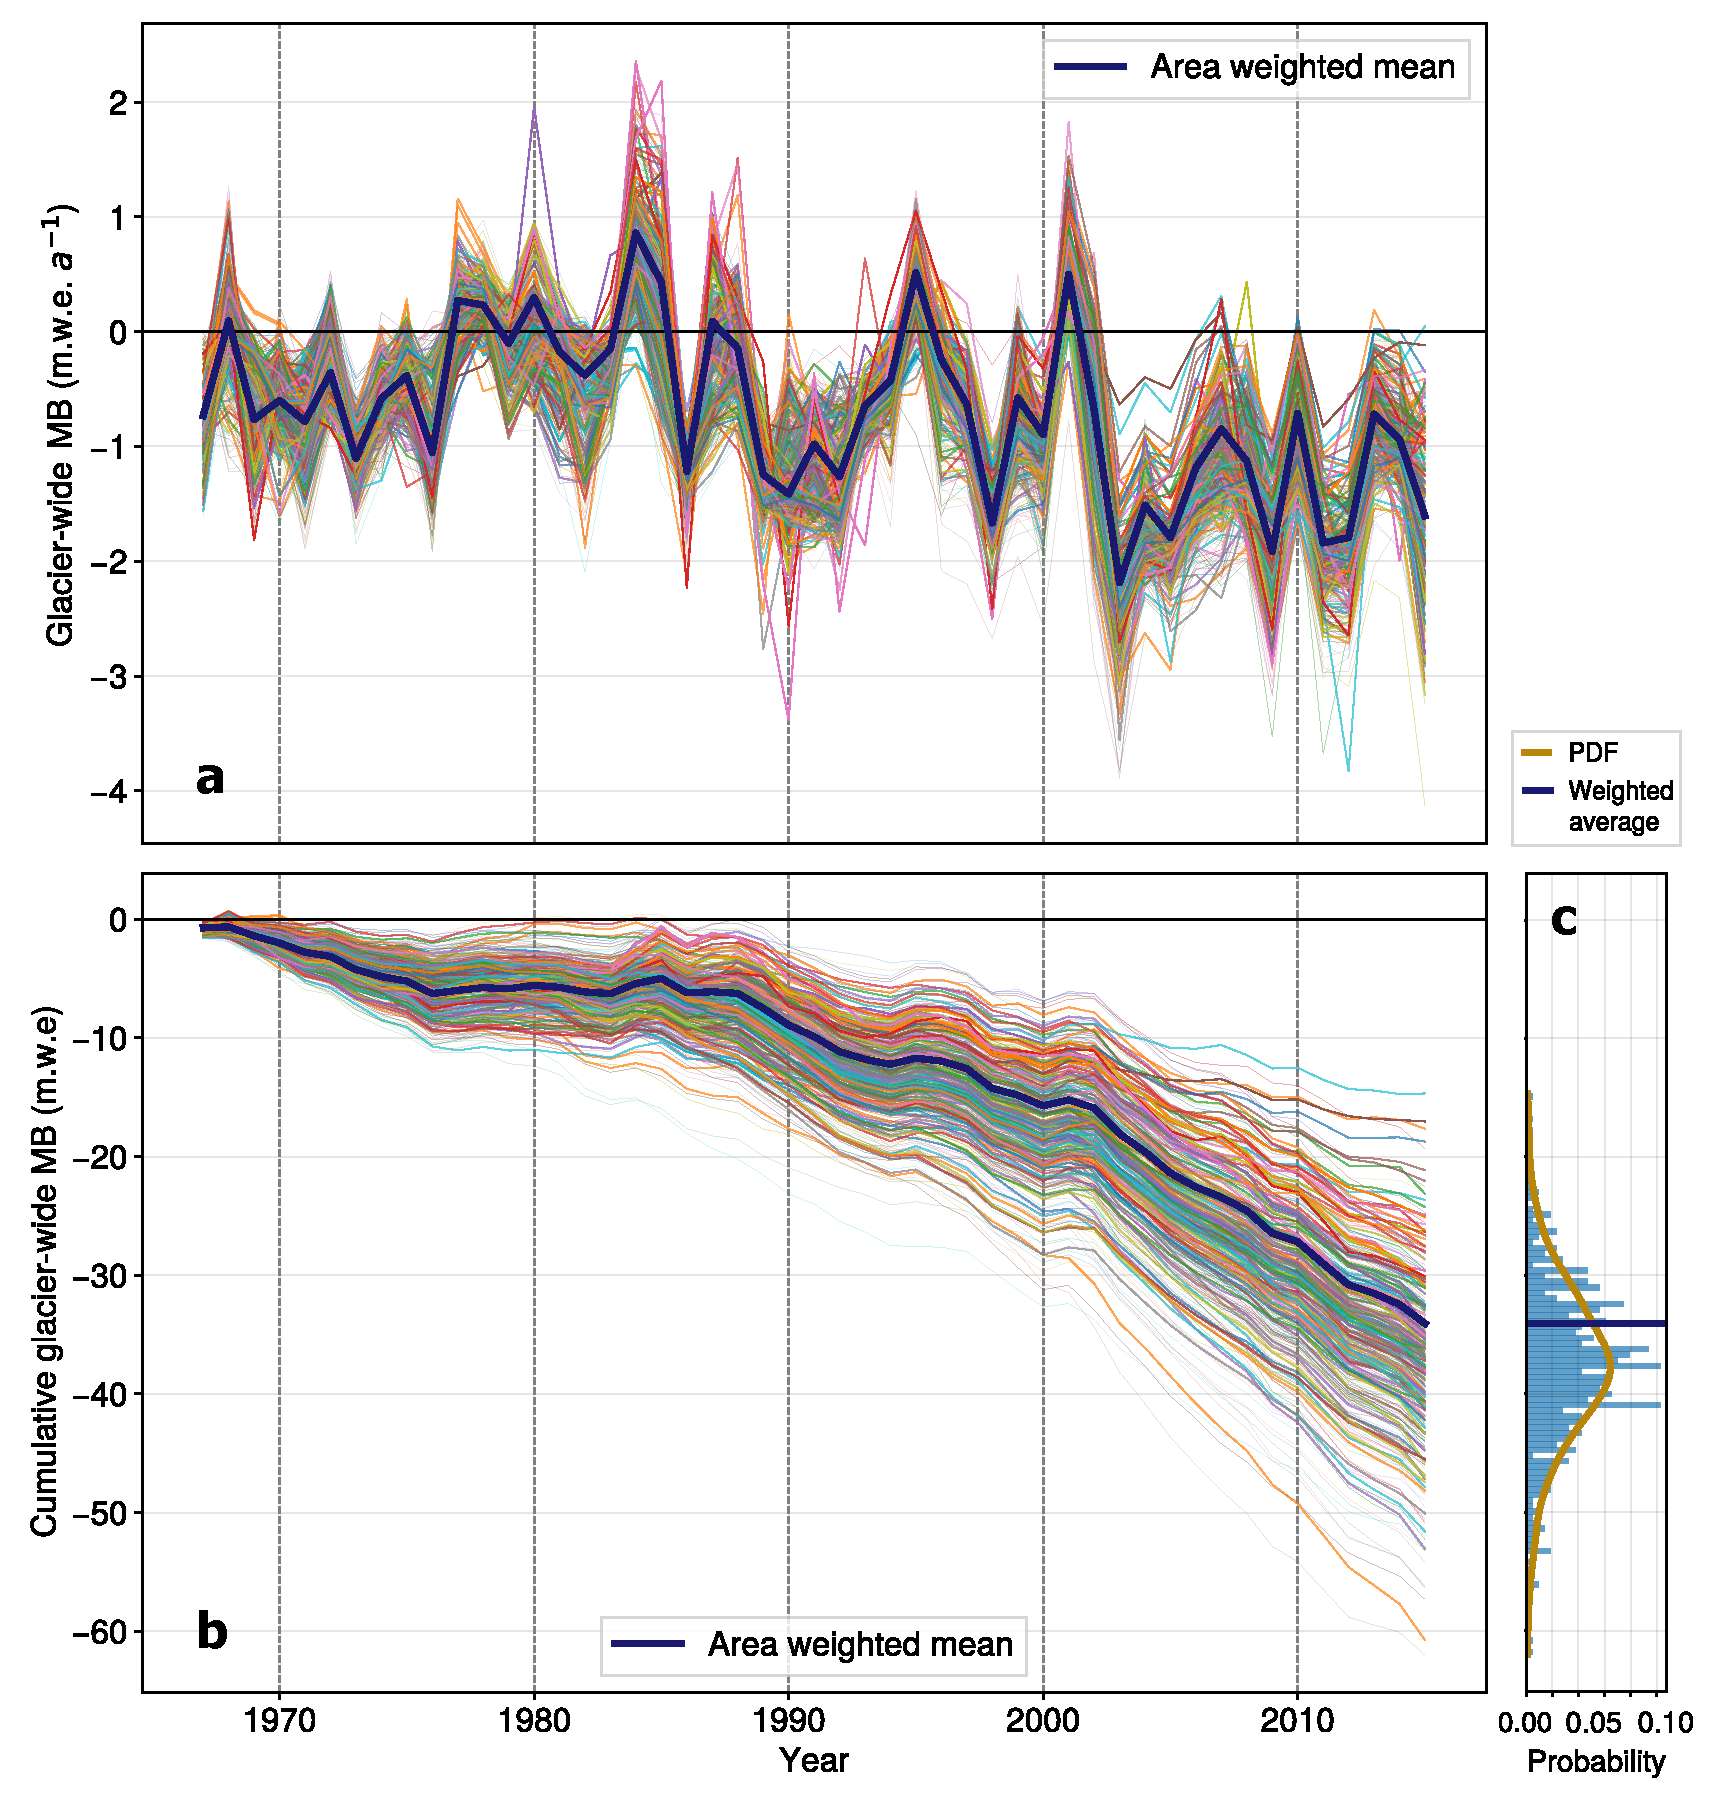
\includegraphics[width=11cm]{Figures/past/Figure_3.pdf}
\captionsetup{justification=centering}
\caption{(a) Annual glacier-wide MB and (b) cumulative glacier-wide MB reconstructions of all the glaciers in the French Alps ($N$ = 661) between 1967 and 2015. For each individual glacier, line thickness depends on glacier area, with smaller glaciers having thinner lines. The histogram (c) indicates the distribution and probability density function (PDF) of the 1967-2015 cumulative MB (m w.e.) of the dataset.}
\label{past:fig3}
\end{figure}

\subsection{Overall trends} \label{past:overview:overall}

We estimate an average area-weighted regional glacier-wide MB of -0.69±0.21 ($\sigma$) m.w.e. a$^{-1}$ between 1967 and 2015 (Fig. \ref{past:fig3} and \ref{past:fig4}). As reported in previous studies \citep{huss_extrapolating_2012, rabatel_spatio-temporal_2016, vincent_common_2017}, our reconstructed MB data show a slightly negative average value during the 1970s, even less negative in the 1980s, and then increasingly negative values in recent decades with an abrupt change in 2003 (Fig. \ref{past:fig2}). For this period (1967-2015), the year 2003 with its remarkable heatwave remains the most negative glacier-wide MB year (-2.26 m.w.e. a$^{-1}$ on average), with 1984 being the most positive year of the study period (+0.85 m.w.e. a$^{-1}$ on average). The area-weighted average MB is slightly less negative than the mean annual glacier-wide MB, showing a light asymmetry in the probability distribution function (PDF) (Fig. \ref{past:fig3}c). 

\begin{figure}[t]
\centering
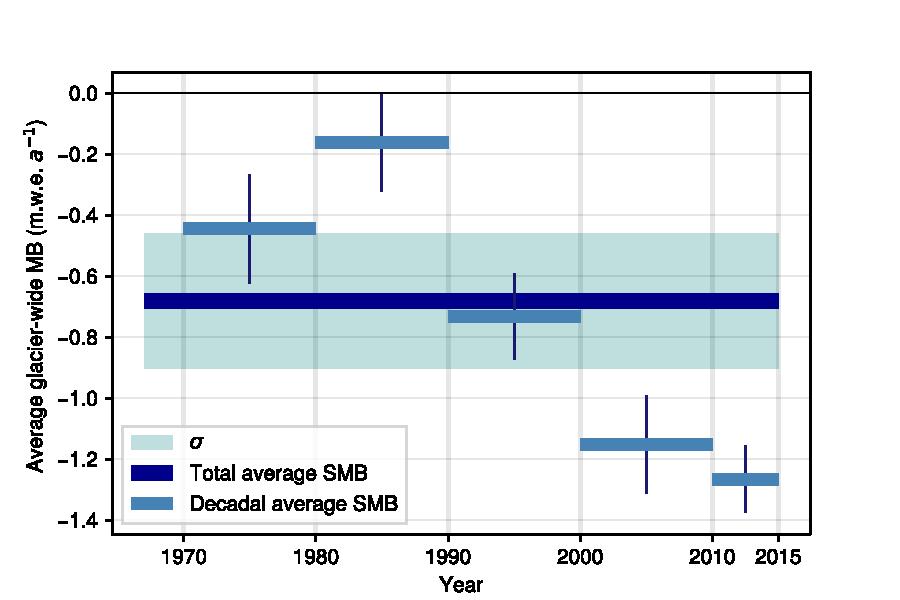
\includegraphics[width=11cm]{Figures/past/Figure_4.pdf}
\captionsetup{justification=centering}
\caption{Averaged area-weighted decadal glacier-wide MB for the French Alps with decadal uncertainties.  The total area-weighted glacier-wide MB is estimated for the 1967-2015 period.}
\label{past:fig4}
\end{figure}

\subsection{Regional and topographical trends} \label{past:overview:regional}

Here we analyse the main trends for the glacierized massifs and for some relevant topographical parameters. The reported glacier-wide MBs are only area-weighted if specifically mentioned. Interesting differences appear once the dataset is divided into mountain ranges (Fig. \ref{past:fig5}). The Mont-Blanc massif presents the lowest mass loss over the entire study period, with an average cumulative loss over the 1967-2015 period of 33.5 m.w.e. This is probably due to its northern location within the French Alps and its large high altitude accumulation areas, which resulted in more positive or less negative MBs, especially during the 1980-2000s. Oisans is the massif with the second lowest average cumulative mass loss (37.20 m.w.e.). Its glaciers have average altitudes ranging from 2290 to 3470 m.a.s.l., with around 50\% of them having mean altitudes over 3000 m.a.s.l. and with about 40\% of glaciers (including most of the large ones) having a northern aspect. Glaciers in Haute-Tarentaise present similar characteristics to those from Oisans, with mean altitudes ranging between 2300 and 3600 m.a.s.l., with about 60\% of the glaciers above 3000 m.a.s.l. This less negative trend was especially important during the recent years with high mass losses from 2003 onwards. On the other hand, the Ubaye, Champsaur, Chablais and Haute-Maurienne massifs appear as the most affected mountain ranges with cumulative mass losses reaching between 41 and 46 m.w.e. for the four massifs over the 1967-2015 period. The Chablais range has a very small number of glaciers remaining, all of them at rather low altitudes (2200-2900 m.a.s.l.), relatively small (0.01 - 1.1 km$^{2}$), and with a northwestern aspect. Despite being the northernmost mountain range in the French Alps, its low altitude is most likely the main reason for the very negative MBs, which were under the regional average even during the positive years in the 1980s. The Champsaur range shows a similar situation, with very small glaciers (0.03 - 0.89 km$^{2}$) lying at relatively low altitudes (2300-3100 m.a.s.l.) in the southernmost latitudes of the Alps (44º7’). Finally, the situation of the Ubaye massif is quite similar to the one of Champsaur, being the southernmost glacierized massif in the French Alps, with a strong mediterranean influence. Such glaciers are remnants of the Little Ice Age, far from being in equilibrium with the warming climate, and can quickly lose a lot of mass through non-dynamic downwasting \citep{paul_rapid_2004}.

When classifying the MB time series by glacier surface area, we encounter the following patterns, with $n$ being the number of glaciers in the subset and $s$ its standard deviation: (1) Very small glaciers (< 0.5 km$^{2}$; $n$ = 534; $\overline{MB}_{1967-2015}$ = -0.79 m.w.e. a$^{-1}$; $s$ = 0.23 m.w.e. a$^{-1}$) present more negative glacier-wide MBs than (2) small/medium glaciers (ranging from 0.5 to 2 km$^{2}$; $n$ = 93; $\overline{MB}_{1967-2015}$ = -0.74 m.w.e. a$^{-1}$; $s$ = 0.18 m.w.e. a$^{-1}$) and (3) large glaciers (> 2 km$^{2}$; $n$ = 34; $\overline{MB}_{1967-2015}$ = -0.68 m.w.e. a$^{-1}$; $s$ = 0.14 m.w.e. a$^{-1}$) (Fig. \ref{past:figS8}). Very small glaciers present a larger spread of values than small/medium and large glaciers ($s$ = 0.23 m.w.e. a$^{-1}$ versus 0.18 and 0.14 m.w.e. a$^{-1}$, respectively). As explained in Sect. \ref{past:methods}, the uncertainties for very small glaciers are greater due to their under-representation in the training dataset, meaning that analyses based on small glaciers have to be taken with greater care. The effects of these trends can be seen in the PDF of the cumulative MB reconstructions (Fig. \ref{past:fig3}c), where the area-weighted mean lies slightly outside the PDF maximum, showing how a great number of small glaciers are presenting higher losses. On the other hand, a clearer relationship between the glacier slope (computed here as the lowermost 20\% altitudinal range slope) and glacier-wide MB arises, with steeper glaciers having less negative glacier-wide MBs (Fig. \ref{past:figS6} and \ref{past:figS9}). Glaciers with a gentle tongue slope generally present longer response times and higher ice thickness, which are associated with more negative mass balances \citep{hoelzle_secular_2003, huss_sensitivity_2016, zekollari_imbalance_2020}. These results are in agreement with the findings by \citet{fischer_surface_2015}, who computed the geodetic mass balance of all the Swiss glaciers for the 1980-2010 period. Overall, the topographical relationships found here are similar, although more negative than for the Swiss Alps \citep{huss_extrapolating_2012, huss_new_2015-2}, showing how the southernmost glaciers in the Écrins and Vanoise regions present stronger glacier mass losses. This is mostly due to their mediterranean climatic influence compared to the more continental Swiss and Austrian glaciers, which results in more negative MB in a warming climate \citep{oerlemans_relating_2000}. Nonetheless, results from this type of bivariate analysis can show rather biased trends, since the topographical variables are highly intercorrelated, with for example small glaciers having steeper slopes and \textit{vice versa} \citep{gardent_multitemporal_2014}. The position and evolution of the equilibrium line can totally reverse the trends of small or steep glaciers, so these relationships can strongly vary depending on the region or time period observed. 


\begin{figure}[t]
\centering
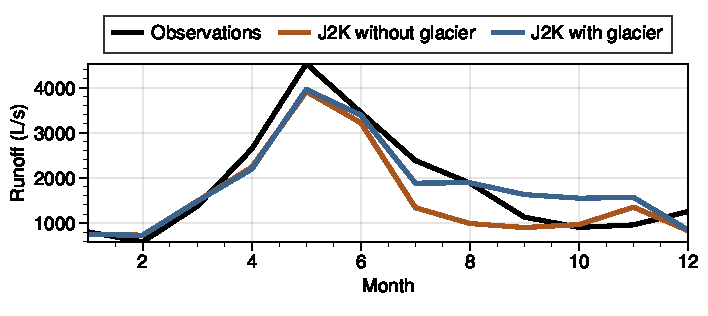
\includegraphics[width=15cm]{Figures/past/Figure_5.pdf}
\captionsetup{justification=centering}
\caption{(a) Averaged annual glacier-wide MB and (b) cumulative averaged glacier-wide MB time series for each of the massifs in the French Alps between 1967 and 2015. (c) Glacierized massifs in the French Alps with the average glacier-wide MB for the 1967-2015 period. Coordinates of bottom left map corner: 44º32' N, 5º40' E. Coordinates of the top right map corner: 46º08' N, 7º17' E.}
\label{past:fig5}
\end{figure}

\subsection{Comparison with previous studies and observations} \label{past:overview:comparison}

In order to put into perspective the reconstructions presented in this study, we compare them to an updated version from the \citet{marzeion_brief_2015} reconstructions (B. Marzeion, personal communication, October 2019 - January 2020), and to all the available glacier-wide MB observations and remote sensing estimates in the French Alps. The goal of this comparison is not to draw conclusions on the quality of either reconstruction, but to analyse the differences among them and to try to understand the causes. In the updated version of \citet{marzeion_brief_2015} - referred as $M_{15U}$ from now on -  a global MB model relying on temperature and solid precipitation was used to reconstruct MB time series for all the glaciers in the world present in the Randolph Glacier Inventory \citep{consortium_randolph_2017}. This model was optimized based on five parameters: the temperature sensitivity of the glacier (local); and a precipitation correction factor, precipitation lapse rate, temperature threshold for solid precipitation and melt temperature threshold (global). As in \citet{bolibar_deep_2020-1}, the approach by $M_{15U}$ was cross-validated respecting the spatiotemporal independence in order to evaluate its performance for unobserved glaciers and years. Due to the highly different methodologies and forcings of the two models, a direct comparison is not possible, so the following analysis is focused on the overall trends and sensitivities in the reconstructions and their potential sources. All the specific differences and details between the two models can be found in Sect. \ref{past:supp:diff} from the Supplement. 

The annual variability (Fig. \ref{past:fig6}), driven by climate, is quite similar between the two reconstructions. Conversely, important differences are found for different subperiods in the amplitude of the area-weighted mean glacier-wide MB series. These differences are the greatest in the 1970s, 1980s and 2010s, with similar average values for the 1990s and 2000s (Fig. \ref{past:fig6} and \ref{past:figS7}). $M_{15U}$ presents less negative and more positive glacier-wide MB values in the 1970s, but on the contrary, it presents more negative values in the 1980s compared to our results. We believe there might be two potential reasons for this: (1) In 1976 there was a shift in the winter mass balance regime in the French Alps, with more humid winters bringing more accumulation; and in 1982 there was a shift in the summer mass balance, resulting in increased ablation \citep{thibert_climatic_2013}. Since both models use parameterized or statistical relationships for MB response to precipitation and temperature, they are likely to react differently to these changes. A similar situation is found from the year 2003 onwards, where there was a substantial increase in temperatures and mass loss \citep[e.g.][]{six_sensitivity_2014}. Our reconstructions show a marked change in 2003 (change of slope in the cumulative plot in Fig. \ref{past:fig6}), whereas $M_{15U}$ present a rather linear trend. The fact that $M_{15U}$ used a volume-area scaling compared to the interpolated topographical data from inventories from this study means that the topographical feedback of the models might differ as well throughout the reconstructed period. (2) For the 1967-1983 interval, the amount of available glacier-wide MB data for training is much lower than for the rest of the period (green numbers in Fig. \ref{past:fig6}). This is likely the reason why the differences between our reconstructions and training data are greater for that period (Fig. \ref{past:fig6}). On the other hand, the similarities between our reconstructions and the training data for the 1984-2014 period are explained by the fact that the 32 glaciers with observations represent around 45\% of the total glacierized area in the French Alps in the year 2003. For the periods before and after this interval, differences and uncertainties in the reconstructed values are greater because of the smaller sample size.

\begin{figure}[t]
\centering
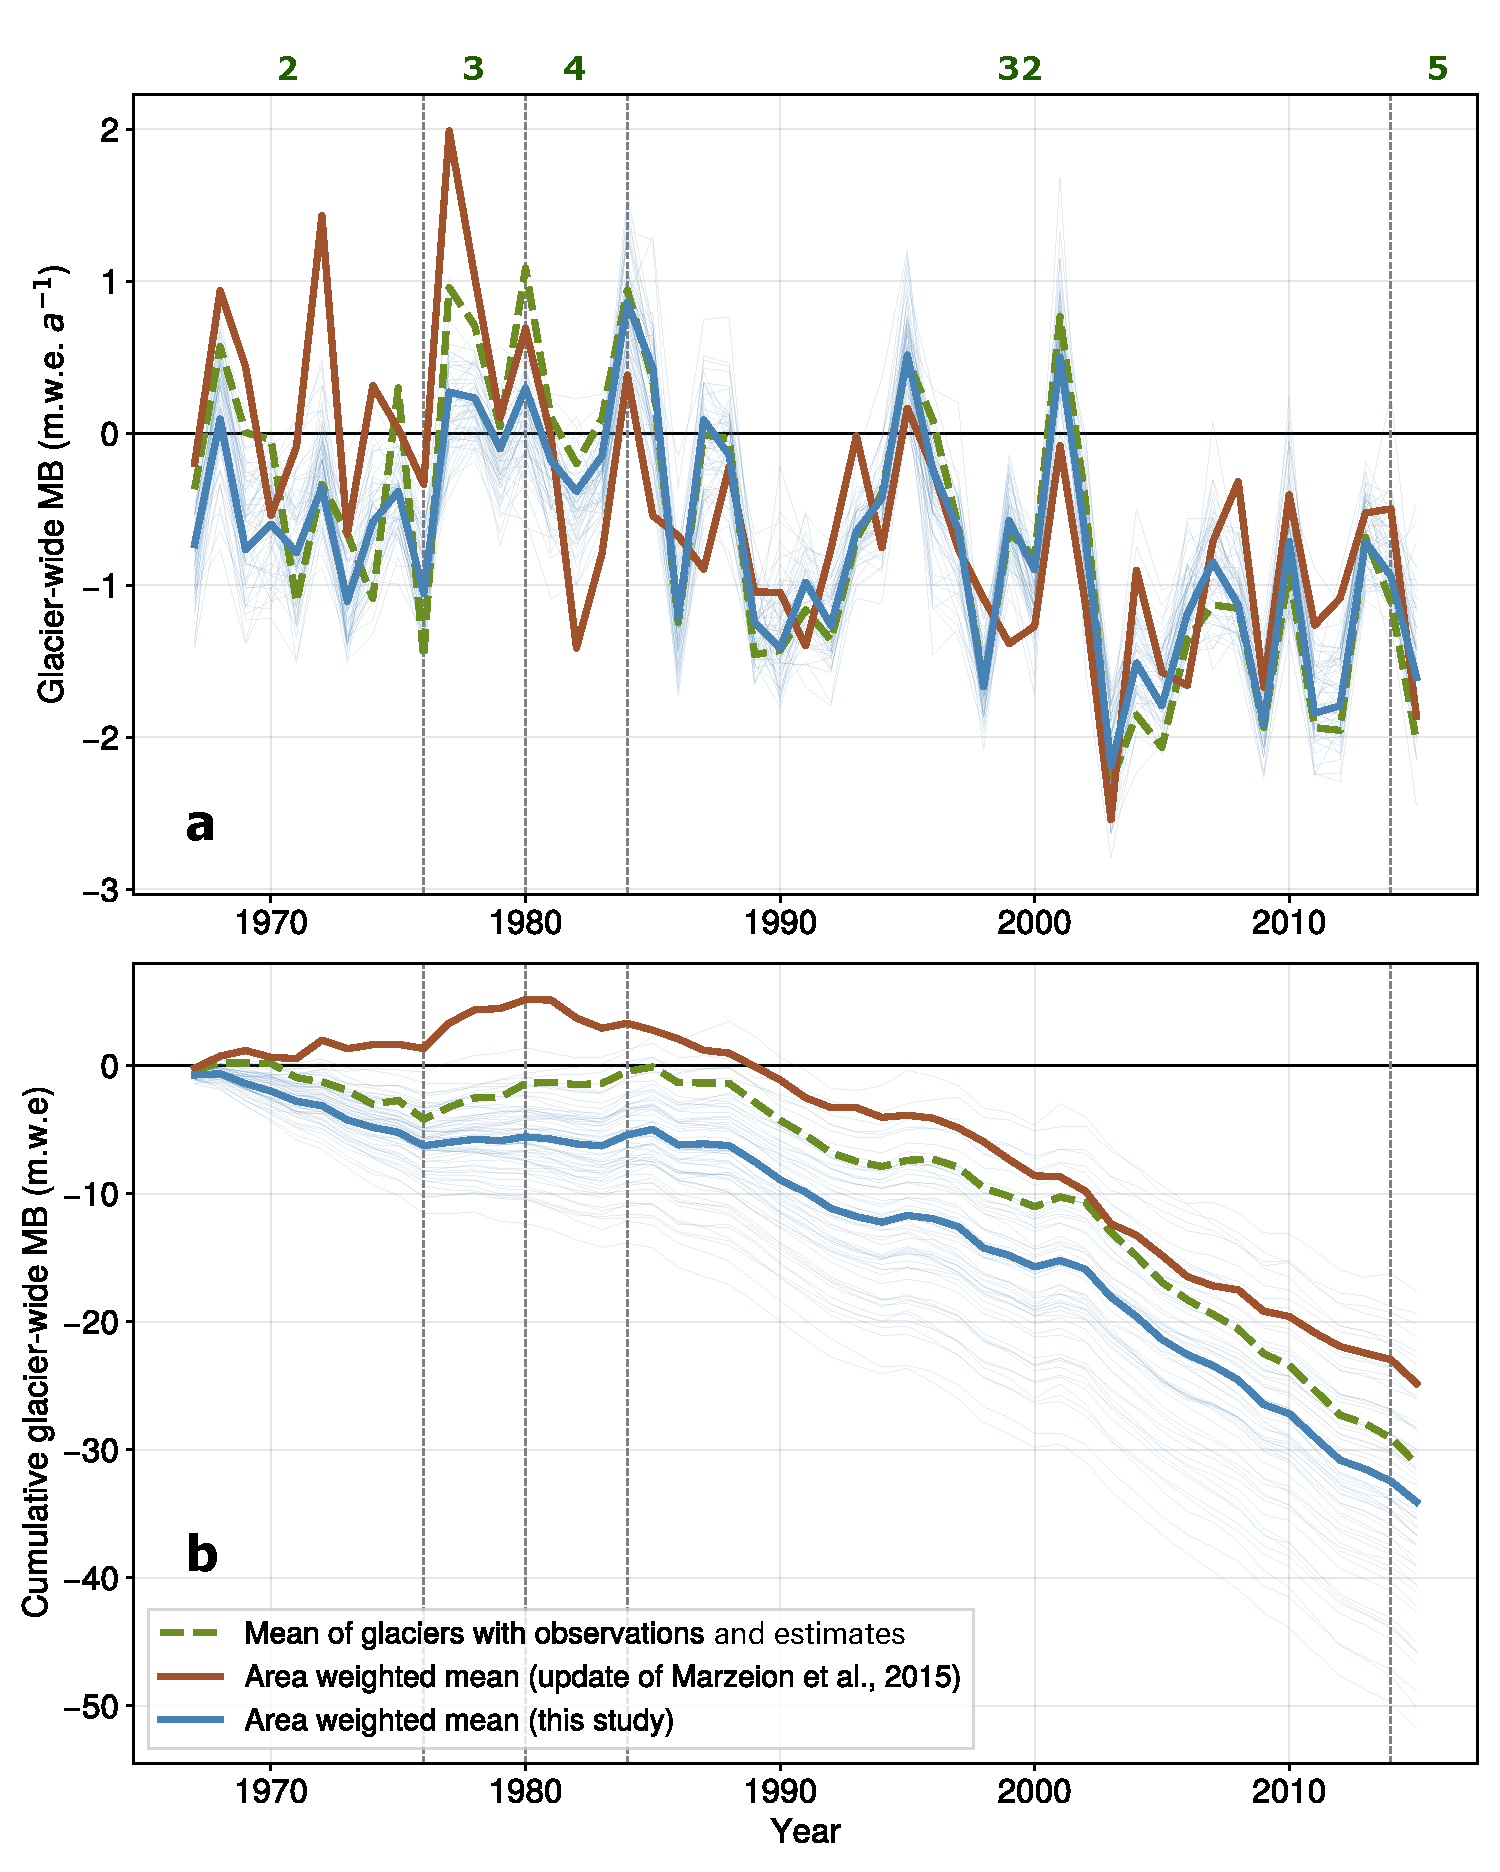
\includegraphics[width=10cm]{Figures/past/Figure_6.pdf}
\captionsetup{justification=centering}
\caption{Comparison of (a) annual and (b) cumulative glacier-wide MB simulations in the French Alps between this study, reconstructions from an update from Marzeion et al. (2015) and the mean of all observations and remote sensing estimates available in the French Alps. Green numbers indicate the number of glaciers with MB observations and remote sensing estimates for each period and thin light blue lines indicate the area-weighted mean of each of the cross-validation ensemble members.}
\label{past:fig6}
\end{figure}

In the following, we argue that similarities between observations, remote sensing estimates and the reconstructed glacier-wide MB values for the 1984-2015 period in this study (Fig. \ref{past:fig6}) are not due to overfitting. First, for the vast majority of the 661 French glaciers, the reconstructions are based on an ensemble of cross-validated models, which intrinsically limits overfitting (Sect. \ref{past:methods}).  Second, we analysed the deviation to the climatological mass-balance signal of the MB for each cluster of glacier-sizes. This analysis is presented in Sect. \ref{past:supp:overfitting} of the supplementary material. It reveals that the similarities between the training data and the reconstructed glacier-wide MB values for the 1984-2015 period in Fig. \ref{past:fig6} originate from big glaciers, that dominate both in the area-weighted reconstructions and in the training data (Fig. \ref{past:figS3} and \ref{past:figS4}). However, for the other glacier-size classes, our reconstruction shows different patterns from the data in the training data, which suggests that the model is not overfitting (Fig. \ref{past:figS3}). 

\section{Conclusions} \label{past:conclusions}

We presented a dataset of annual glacier-wide MB of all the glaciers in the French Alps (44° - 46°13’N, 5.08° - 7.67°E) for the 1967-2015 period \citep{bolibar_deep_2020}. This dataset has been reconstructed using deep learning (i.e. an artificial neural network), based on direct and remote sensing annual glacier-wide MB observations and estimates, climate reanalysis and topographical data from multitemporal glacier inventories. The deep learning model is capable of reconstructing glacier-wide MB time series for unobserved glaciers in the same region based on patterns and structures learnt by the artificial neural network from the training data and their relationships with predictors. An extensive cross-validation was implemented to understand the characteristics of the MB signal in the region and to assess the method’s validity and uncertainty. The average accuracy (RMSE) of the dataset is estimated at 0.55 m.w.e. a$^{-1}$ with an explained variance ($r^{2}$) of 75\%. Reconstructions show a mean area-weighted glacier-wide MB of -0.69±0.21 (1 $\sigma$) m.w.e. a$^{-1}$ for the 1967-2015 period. Important differences are found among different massifs, with the Mont-Blanc (-0.68 m.w.e. a$^{-1}$), Oisans (-0.75 m.w.e. a$^{-1}$ both) presenting the lowest mass losses and the Chablais (-0.93 m.w.e. a$^{-1}$), Champsaur (-0.86 m.w.e. a$^{-1}$) and Haute-Maurienne and Ubaye (-0.84 m.w.e. a$^{-1}$ both) showing the highest losses. In order to put these results into perspective, this reconstruction was compared to all available glacier-wide MB observations and remote sensing estimates in the French Alps as well as the physical/empirical reconstructions from another study \citep[update from][]{marzeion_brief_2015}. Interesting differences were found between the two methods, highlighting the different sensitivities and responses of different approaches to climate shifts that occurred during the study period. These differences are particularly relevant in the 1970s and 1980s, previous to a winter precipitation and summer temperature shift that occurred in the French Alps in the years 1976 and 1982, respectively. Moreover, after the famous 2003 European heatwave, glaciers experienced an acceleration in mass loss which is well captured by our reconstruction. This open glacier-wide MB dataset can be useful for hydrological or ecological studies in need of net glacier mass contributions of glacierized catchments in the French Alps. The publication of such open datasets is essential to future community-based data-driven scientific studies.

\section{Supplementary material}

\begin{figure}[h]
\centering
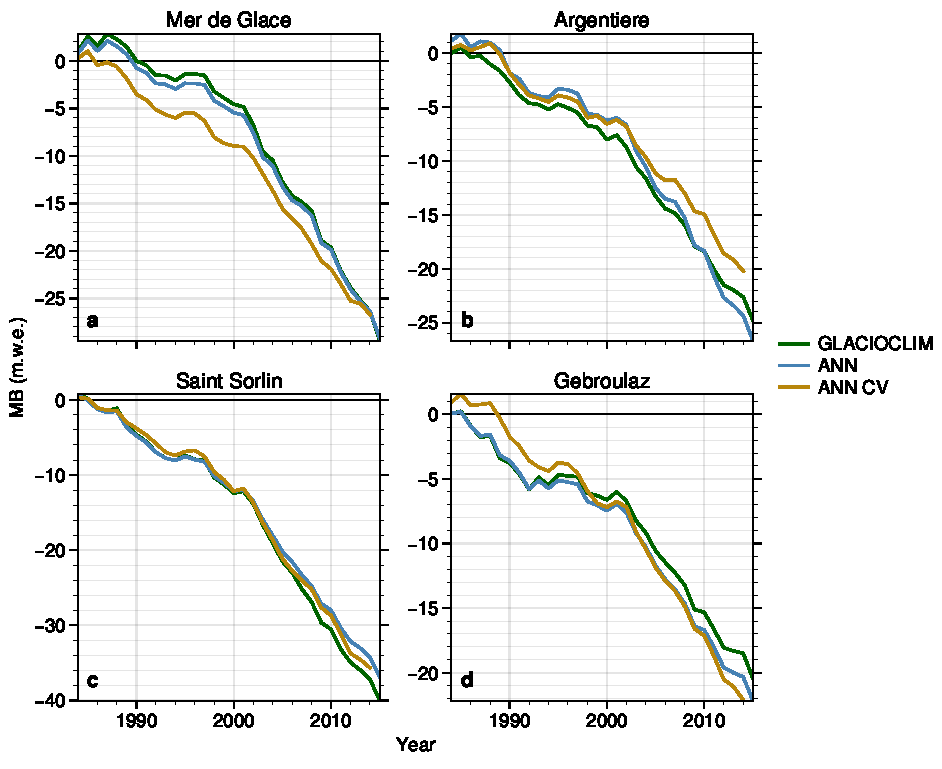
\includegraphics[width=12cm]{Figures/past/Figure_S1.pdf}
\captionsetup{justification=centering}
\caption{Comparison between glaciological observations from the GLACIOCLIM observatory, cross-validated MB reconstructions from this study (ANN CV) and fitted MB reconstructions (ANN). The cross-validated models are shown to display the out-of-sample performance. The fitted reconstructions display the actual reconstructions from the dataset, with models especially fitted for glaciers with data.}
\label{past:figS1}
\end{figure}

%\copyrightstatement{TEXT}

\subsection{Comparison with independent geodetic mass balance data} \label{past:supp:comparison}

All available annual glacier-wide MB data in the French Alps have been used to train the MB ANN of the present study. However, some multi-annual geodetic mass balance (MB) datasets exist that can provide a means to validate the reconstruction's bias for specific glaciers during multi-annual time intervals. This type of analysis is more limited than the cross-validation done to annual glacier-wide MB values in \cite{bolibar_deep_2020-1}, as it only gives information about the bias of a sub-period of the reconstructions instead of the accuracy found via cross-validation. Our MB reconstructions are compared against ASTER geodetic MB from \citet{davaze_region-wide_2020} for the 2000-2015 and 2003-2012 periods (Fig. \ref{past:fig2} and \ref{past:figS2}) and against Pléiades geodetic MB from \citet{berthier_glacier_2014} for the 2003-2012 period (Fig. \ref{past:figS2}).

For certain glaciers, the ASTER and Pléiades geodetic MB give a less negative MB than the glaciological SMB used to train the deep learning SMB model. This fact might explain the slightly more negative trend of our reconstructions seen for the 2000-2015 and 2003-2012 periods, which experienced very negative MB after the well known summer 2003 heatwave. This is quite surprising, since both the GLACIOCLIM glaciological MB measurements and the annual glacier-wide MB data from Rabatel et al. (2016) have been calibrated with geodetic MB from photogrammetric DEMs, which have a very high spatial resolution. For some regions (i.e. Grandes Rousses), the independent geodetic MB are well within the uncertainty range of our model. However, large and steep glaciers in the Mont-Blanc massif and some other regions, such as Bossons, Talèfre and Tour display important differences. These glaciers have very large and high altitude accumulation areas, not seen in almost any glacier in our training dataset. On the other hand, several small glaciers present very important differences, with ASTER-derived MB being much less negative than our reconstructions. Data for small glaciers carry very large uncertainties, often of the same order of magnitude as the observations themselves. On top of that, flat or dome-type glaciers with large white areas with high reflectance present an important amount of noise, further increasing the associated uncertainty. This means that is quite hard to jump to conclusions from a direct comparison between these glaciers and our reconstructions. The differences and influence of geodetic MB on the calibration of MB series should be properly studied, as they are often not taken into account as an additional uncertainty source. This topic goes beyond the scope of this study, but glacier modelling studies could benefit from integrating this in the list of uncertainties. 

\begin{figure}[t]
\centering
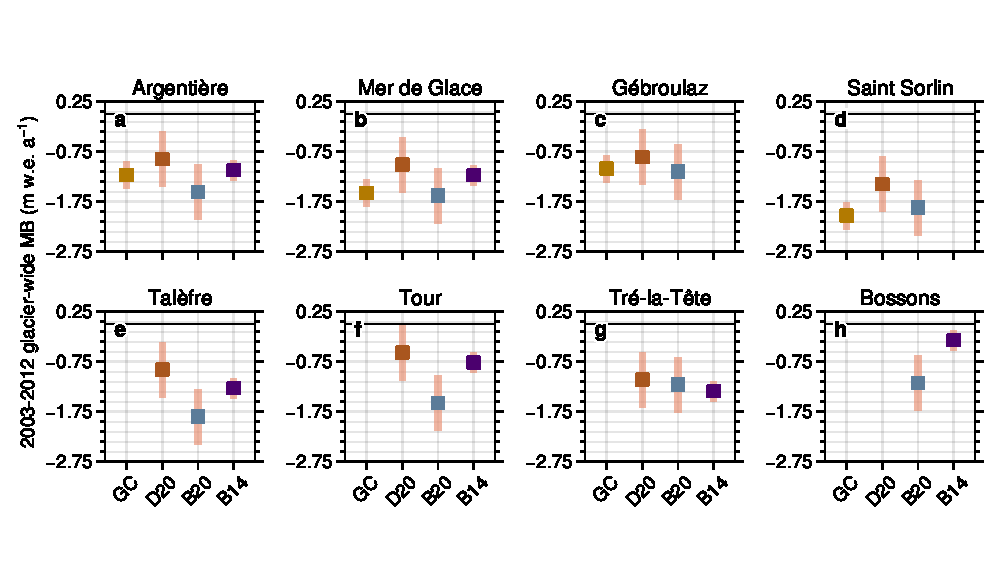
\includegraphics[width=12cm]{Figures/past/Figure_S2.pdf}
\captionsetup{justification=centering}
\caption{Comparison between glaciological observations from the GLACIOCLIM observatory (GC), ASTER geodetic mass balances from Davaze et al. (2020) (D20), the deep learning reconstructions from the present study (B20) and Pléiades geodetic mass balances from Berthier et al. (2014) (B14).}
\label{past:figS2}
\end{figure}

\subsection{Model differences between the updated version of Marzeion et al. (2015) and this study} \label{past:supp:diff}

In order to contrast the results from Sect. \ref{past:overview:comparison}, three important different aspects between our approach and the one of $M_{15U}$ need to be highlighted: 

\begin{enumerate}
\item $M_{15U}$’s model works with simplified physics, with a temperature-index model calibrated on observations; in this study we used a fully statistical approach based on deep learning, where physics-based considerations only appear in the predictor selection.
\item $M_{15U}$ calibrated their model with global MB observations, including 38 glaciers in the European Alps, most of them located in Switzerland for the 1901-2013 period; in this study we used observations of 32 glaciers, all located in the French Alps for the 1967-2015 period.
\item $M_{15U}$ forced their updated model with CRU 6.0 \citep[update of][]{harris_updated_2014}, with 0.5° latitude/longitude grid cells, which has a significantly lower spatial resolution and suitability to mountain areas than the SAFRAN reanalysis \citep{durand_reanalysis_2009} used in this study, in which altitude bands and aspects are considered for each massif, and meteorological observations from high-altitude stations are assimilated.
\end{enumerate}

The cross-validations of both studies determined a performance with an average RMSE of 0.66 m.w.e. $a^{-1}$ and an $r^{2}$ of 0.43 for $M_{15U}$ for the European Alps, and an average RMSE of 0.49 m.w.e. $a^{-1}$ and an $r^{2}$ of 0.79 for this study. However, due to the highly different methodologies and forcings of the two models, a direct comparison is not possible, so the following analysis is focused on the overall trends and sensitivities in the reconstructions and their potential sources. 

\subsection{Influence of area in glacier-wide MB signal and proof on non overfitting} \label{past:supp:overfitting}

Due to similarities between the averaged reconstructed glacier-wide MB and the observations during the 1984-2015 period, we decided to include an analysis to isolate the topographical influence in the glacier-wide MB signal, in order to verify that the model is not overfitting. Since the climate signal is the main common driver of annual variability of glacier-wide MB in the region, one needs to find a way to isolate the topographical signal. In Fig. \ref{past:figS3}, the median reconstructed annual glacier-wide MB of the 661 glaciers in the French Alps (i.e. the annual variability, hence a proxy of the climate signal) is subtracted to the mean annual values of the observations and of 4 subsets of glaciers divided by area classes. Therefore, one can observe the residual influence of glacier area on the glacier-wide MB signal. The influence of area on glaciers with observations is quite similar to glaciers with areas greater than 2 $km^{2}$, which is reasonable since glaciers with observations have an average of 4 $km^{2}$ (range: 0.3-31.8 $km^{2}$ in 2003). Moreover, one can see that even for a relatively short period of 30 years, the differences between the reconstructions for very small glaciers (< 0.5 $km^{2}$) and observations are quite important, accounting for an average cumulative loss of more than 5 m.w.e. As stated in Sect. \ref{past:methods}, this does not necessarily mean that the model has fully captured the topographical influence in the glacier-wide MB signal in the region, but it does prove that the model is not overfitting since it exhibits consistent variations in MB when the topographical predictors move away from the training data. Moreover, this is coherent with the importance attributed to topographical predictors \citep{bolibar_deep_2020-1}. 

The same analysis has been performed with the reconstructions from the updated version of Marzeion et al. (2015) (Fig. \ref{past:figS4}). The gradient with respect to glacier surface area appears to be similar, except for the behaviour of glaciers after 2007. Small and middle sized glaciers (0.1 - 2 $km^{2}$) switch to a positive influence, as opposite to large glaciers (> 2 $km^{2}$), which transition to a negative influence. Conversely, our results show a more continuous trend, without a change of behaviour in the last years of the analysed period. 

\newpage
%\break
\subsection{Supplementary figures}

\begin{figure}[h]
\centering
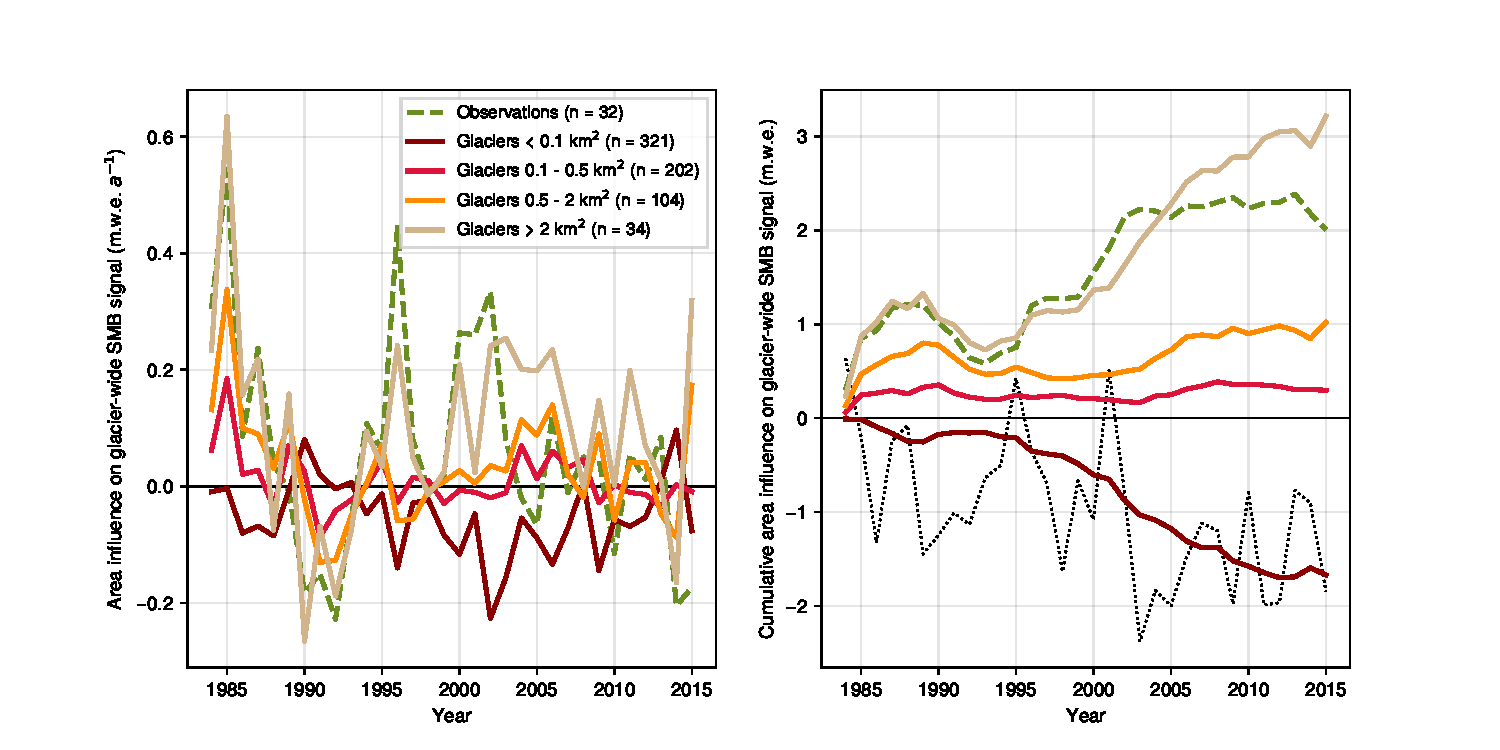
\includegraphics[width=16cm]{Figures/past/Figure_S3.pdf}
\captionsetup{justification=centering}
\caption{Influence of glacier area on the glacier-wide MB signal. The reconstructed median annual glacier-wide MB of the 661 glaciers in the French Alps can be seen as a proxy of the climate signal in the region. It is subtracted to the mean annual glacier-wide MB of the glaciers with observations and to four different subsets of reconstructions divided into glacier area size, showing only the annual differences based on glacier area classes. The dotted line depicts the subtracted signal (non cumulative) in order to give some context.}
\label{past:figS3}
\end{figure}

\begin{figure}[h]
\centering
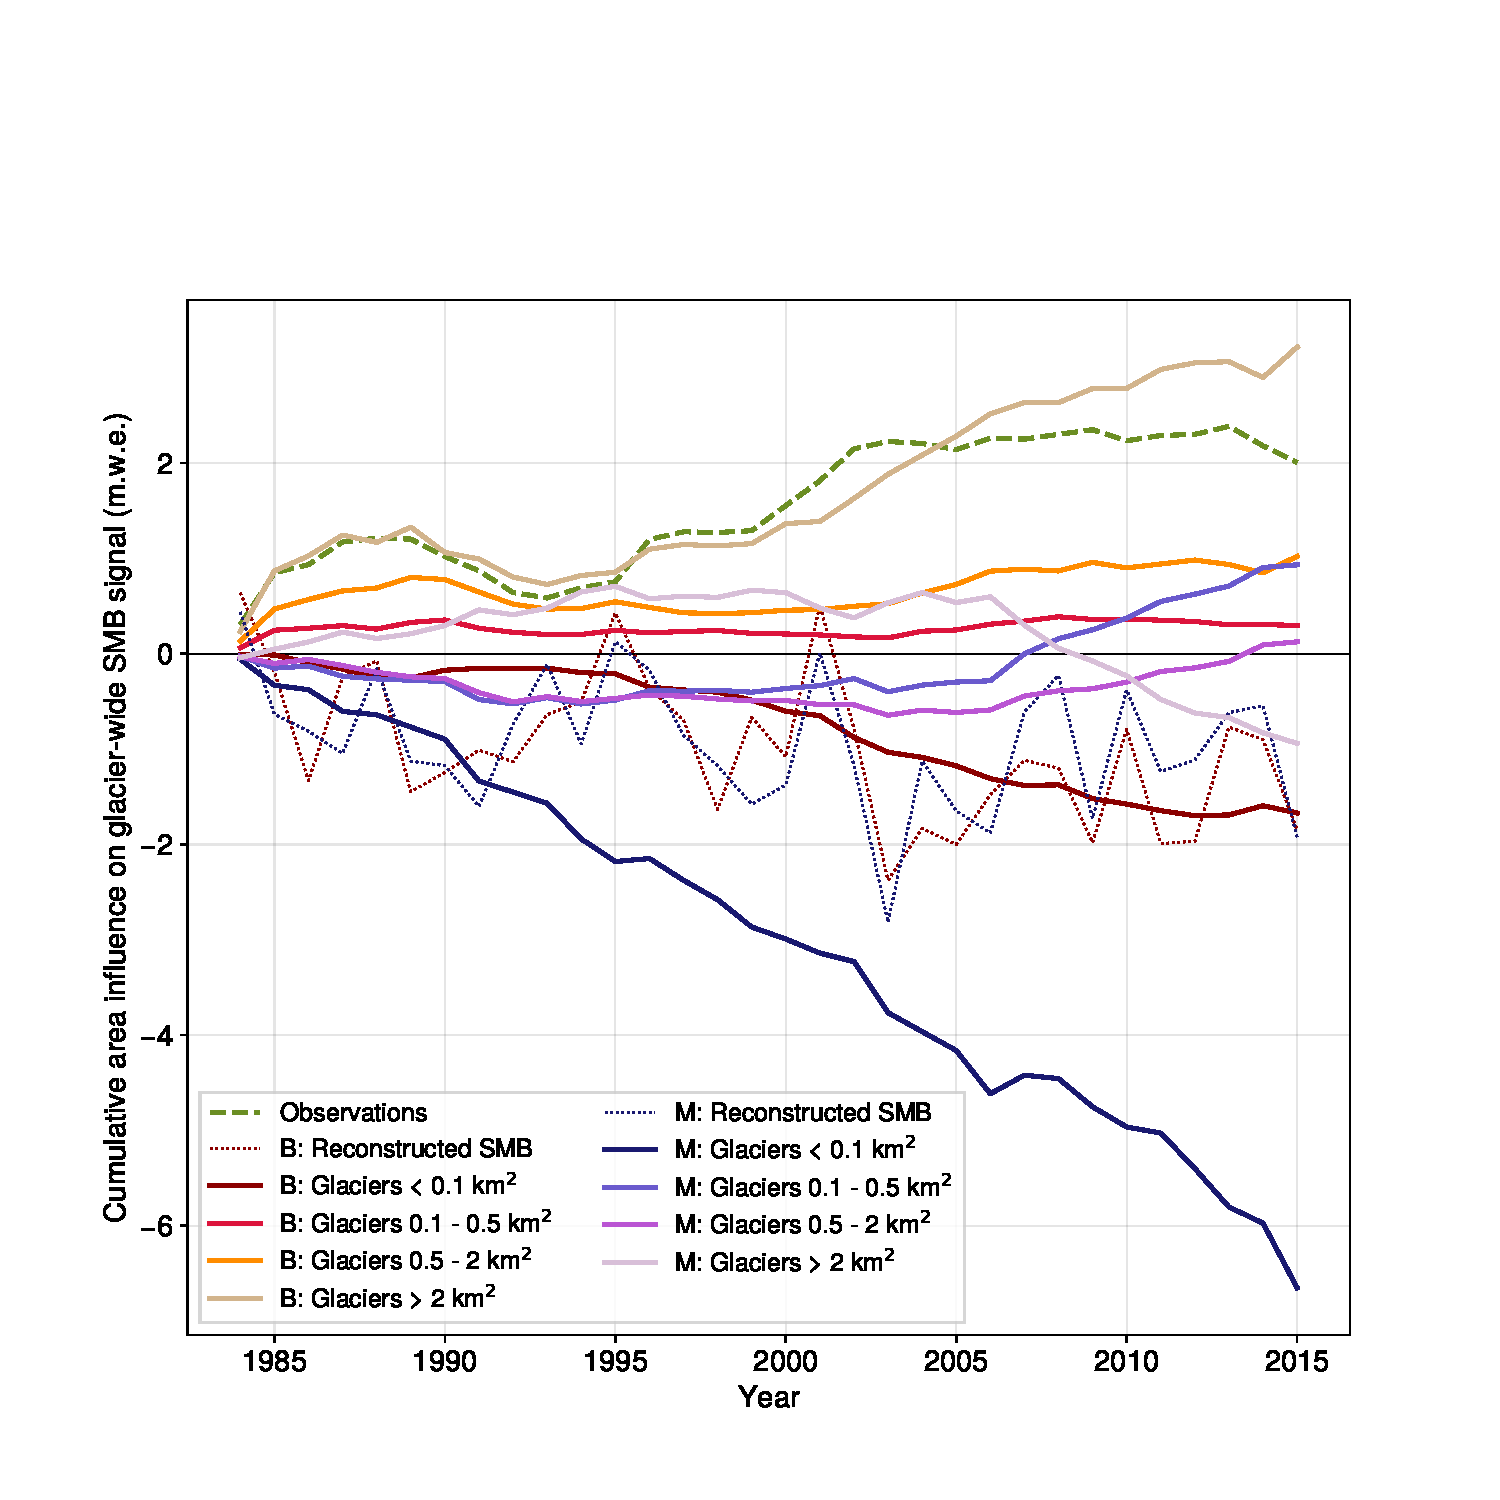
\includegraphics[width=14cm]{Figures/past/Figure_S4.pdf}
\captionsetup{justification=centering}
\caption{Same as S3 but comparing this study to the updated version of Marzeion et al. (2015). In the legend, “B” stands for Bolibar et al. (this study) and “M” for the update of Marzeion et al. (2015). Both models show a relatively similar gradient effect with respect to glacier area, with differences in the amplitude of the effects. The main differences appear from 2007, where small and middle sized glaciers (0.1 - 2 $km^{2}$) from the update of Marzeion et al. (2015) switch to a positive influence, as opposite to large glaciers (> 2 $km^{2}$), which transition to a negative influence. The reconstructed MB dotted lines are not cumulative and they are depicted in order to give some context of the subtracted climate signal.}
\label{past:figS4}
\end{figure}


\begin{figure}[t]
\centering
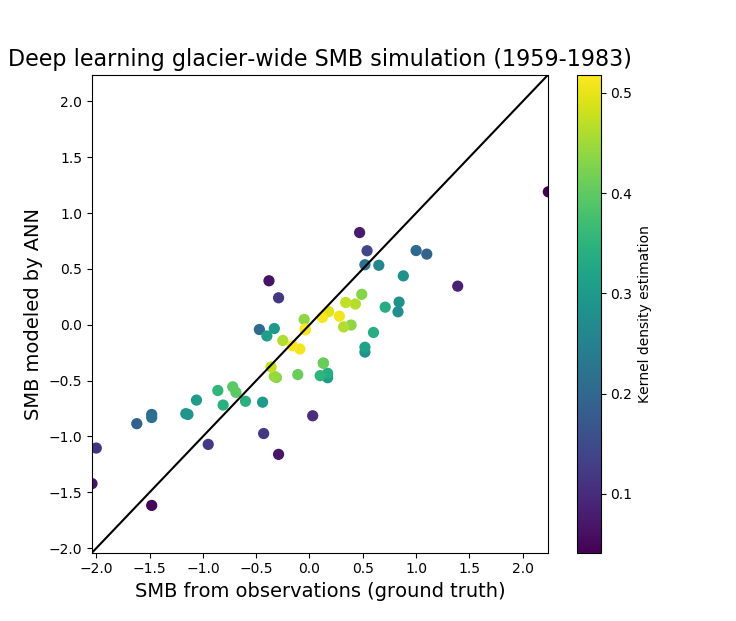
\includegraphics[width=9cm]{Figures/past/Figure_S5.png}
\captionsetup{justification=centering}
\caption{Cross-validation for annual glacier-wide MB values outside the main 1984-2014 training period. The black line indicates the one-to-one reference. Simulations have been done from 1959, the earliest date with observations to validate against the maximum number of values. This serves to confirm that the model is capable of reproducing glacier-wide MB outside the main observed period.}
\label{past:figS5}
\end{figure}


\begin{figure}[t]
\centering
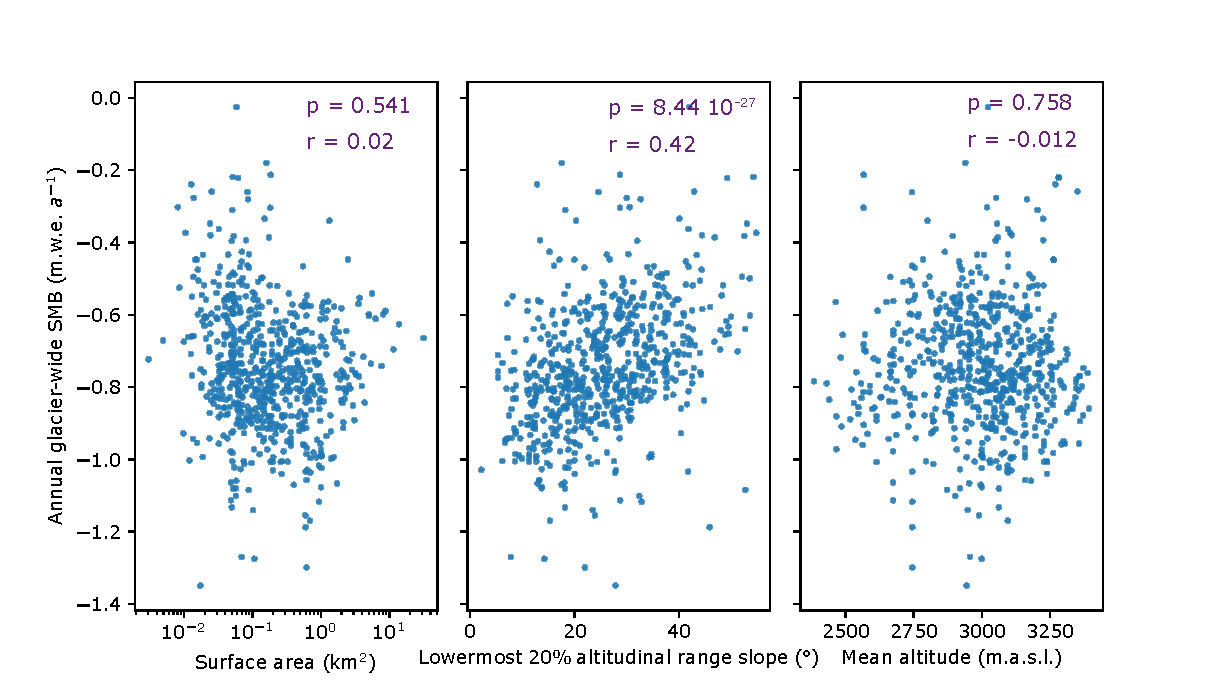
\includegraphics[width=16cm]{Figures/past/Figure_S6.pdf}
\captionsetup{justification=centering}
\caption{Average annual glacier-wide MB for each glacier over the entire study period with respect to (a) glacier surface area, (b) the lowermost 20\% altitudinal range slope and (c) mean glacier altitude. p indicates the p-value and r the correlation between the topographical variables and the average glacier-wide MB.}
\label{past:figS6}
\end{figure}


\begin{figure}[t]
\centering
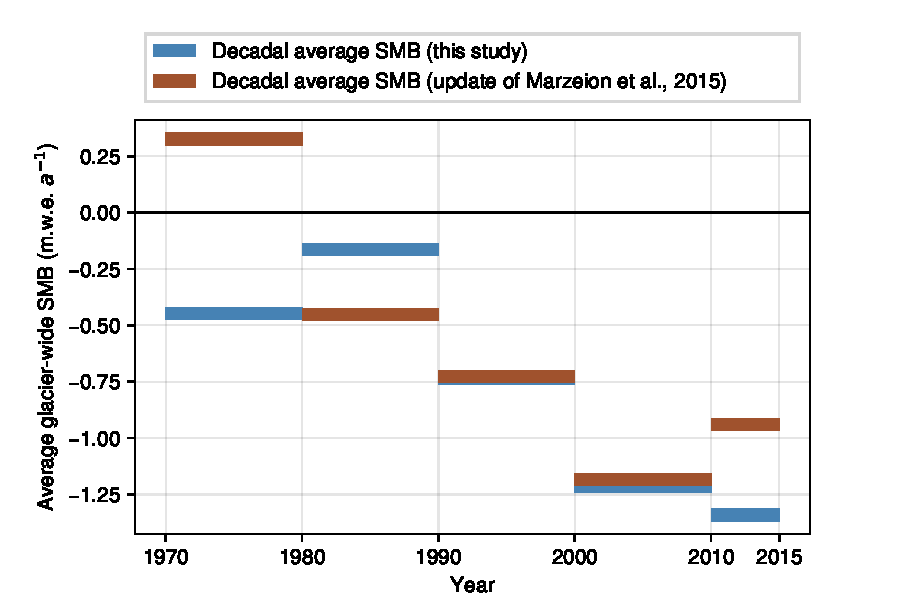
\includegraphics[width=12cm]{Figures/past/Figure_S7.pdf}
\captionsetup{justification=centering}
\caption{Comparison of area-weighted decadal glacier-wide MB simulations in the French Alps between this study and an update from Marzeion et al. (2015).}
\label{past:figS7}
\end{figure}


\begin{figure}[t] 
\centering
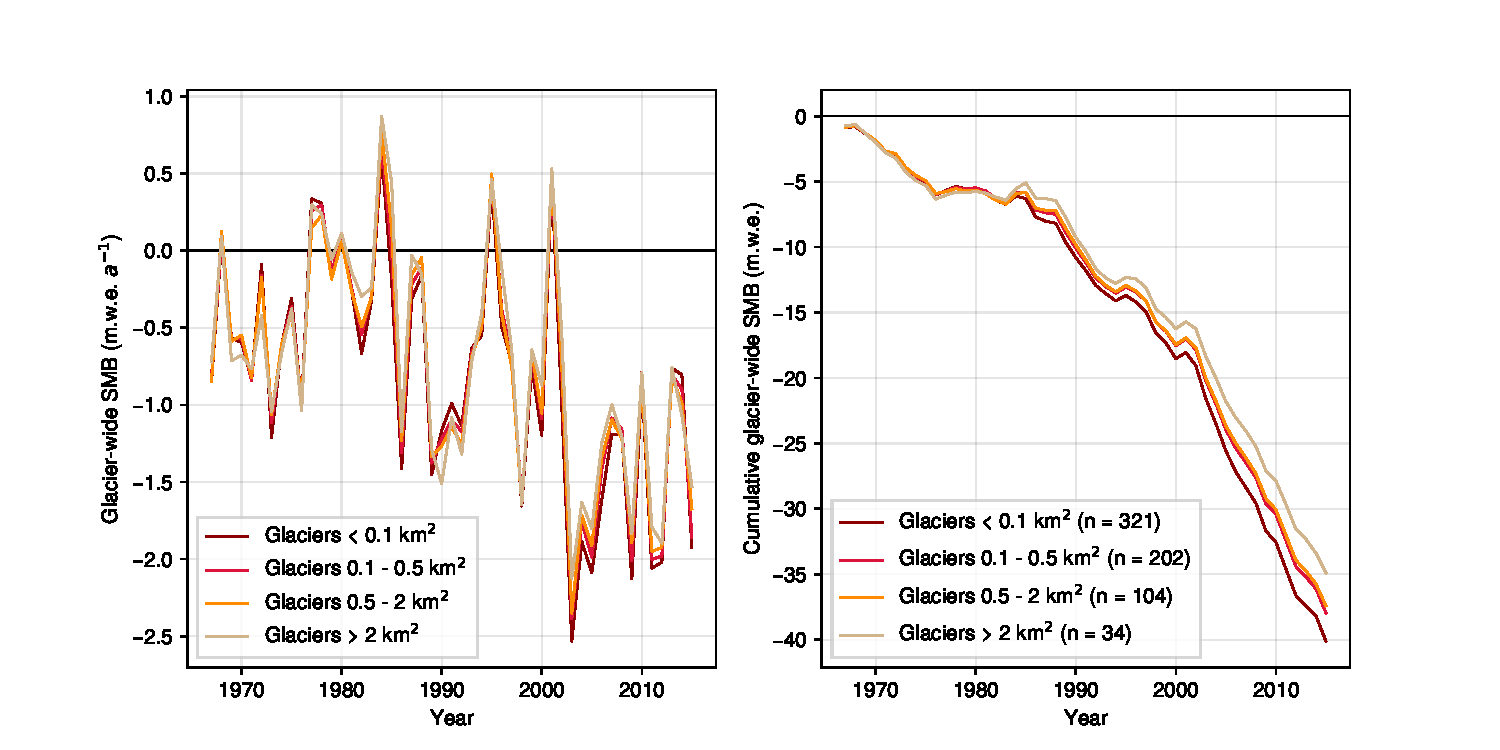
\includegraphics[width=16cm]{Figures/past/Figure_S8.pdf}
\captionsetup{justification=centering}
\caption{Average annual glacier-wide MB per glacier area classes}
\label{past:figS8}
\end{figure}


\begin{figure}[t]
\centering
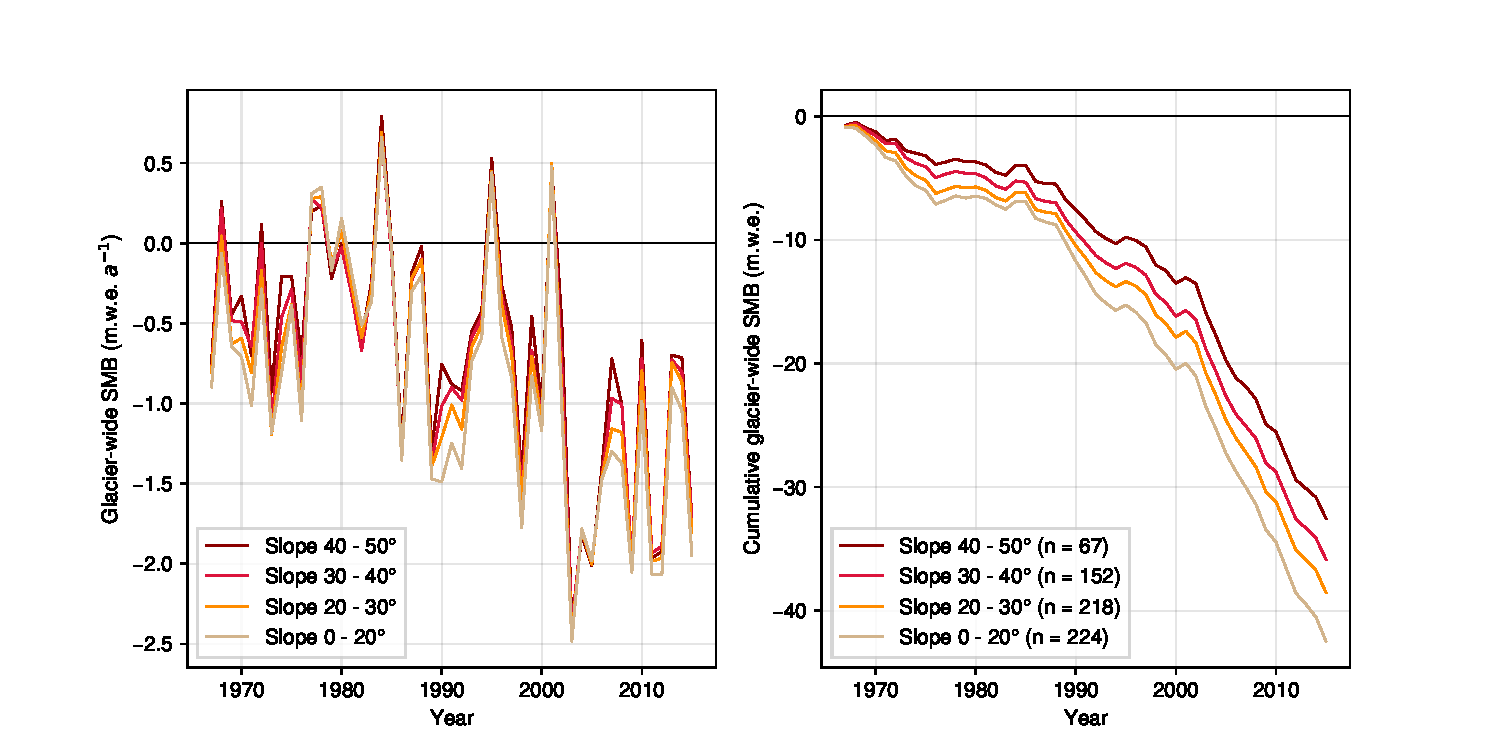
\includegraphics[width=16cm]{Figures/past/Figure_S9.pdf}
%\captionsetup{justification=centering}
\caption{Average annual glacier-wide MB for classes of glacier slope of the lowermost 20\% altitudinal range (i.e. a proxy of the glacier’s tongue slope)}
\label{past:figS9}
\end{figure}



\chapter{The 21$^{st}$ century deglaciation of the French Alps: unraveling climate-glacier interactions with deep learning}
\label{chap:future}

\begin{flushright}
{\small \textit{All models are wrong, but some are useful.}\\
George Box}
\end{flushright}

\section*{Preface}




\part{Glacierized mountain catchments}

\chapter{Hydroglaciological modelling of glacierized mountain catchments}
\label{chap:discussion}

\begin{flushright}
\begin{small}
\textit{In the study of nature, as in the practice of art, it is not given to man to achieve the goal without leaving a trail of dead ends he had pursued.}\\ \\
Baron Louis Bernard Guyton de Morveau
\end{small}
\end{flushright}

\section*{Preface}

This second part dedicated to hydroglaciological modelling is much shorter than the first part dedicated to regional glacier evolution modelling. An unexpected shift in the initial objectives of this PhD project resulted in a lengthy investigation of machine learning methods applied to glacier evolution modelling, which impacted the initial plans for hydroglaciological modelling. Efforts for this part of the PhD work have been focused on the technical implementation and validation of a novel glacier component for a hydrological model. With this implementation, we are providing the technical means for an application on hydroglaciological applications at a regional scale in the French Alps. This work has been done with the help of Sven Kralisch from the University of Jena. His expertise on the hydrological model used in this study has greatly helped to accelerate the development of the new glacier module in the last months of this project.

\section{Introduction}

Glaciers supply water that supports ecosystems and human communities both nearby and far away from glaciers \citep{ipcc_climate_2018}. The strong climatic diversity of glacierized alpine catchments enables the storage of precipitation in the form of snow, firn and ice at high altitudes. This water storage is progressively released throughout the year during the warmest months, providing a more constant runoff than non-glacierized catchments. At the beginning of the melt season, snow provides important water resources downstream. Once most of the snow has melted, leaving bare glacier ice exposed, glaciers continue providing freshwater resources, ensuring an uninterrupted runoff throughout the melt season \citep{huss_toward_2017}. This role of glaciers as late summer buffers is currently being challenged by anthropogenic climate change. Glacier retreat in the European Alps is transforming the hydrological regime of high-mountain catchments, with potential environmental and social impacts \citep{zekollari_modelling_2019}. In the French Alps, the local population have a strong dependency on water resources, using them for the ski business \citep{spandre_winter_2019}, hydropower generation and domestic use. The regional socioeconomic model is built around mountain tourism, with a strong dependency on the cryosphere, both as a tourism attraction \citep{schut_sport_2013} and as an electricity generation source \citep{schaefli_role_2019}. Moreover, late summer runoff from glaciers provides reliable water resources for domestic use, industries and agriculture. This decrease in glacier freshwater contributions has ecological impacts as well, decreasing biodiversity in glacier-fed rivers \citep{cauvy-fraunie_global_2019} and in humid areas that no longer receive runoff during the warmest period of the year \citep{carlson_monitoring_2020}. Glaciers provide cold water resources that help regulate the temperature, flow regimes, sediment concentration and nutrient supply of mountain streams \citep{huss_toward_2017}. These cold waters are essential to some specialized species, whose survival will be challenged by glacier retreat \citep{lencioni_glacial_2018, cauvy-fraunie_global_2019}.  Alternatively, these changing streams can be quickly colonized by aquatic communities adapted to higher water temperatures, increasing competition between species  \citep{robinson_ecosystem_2014}. Anticipating these future hydrological changes is of paramount importance in order to correctly adapt and manage future water social and environmental needs. 

Hydrological models can provide answers to these questions, predicting the hydrological evolution under of different future climate scenarios. In France, multiple hydrological models are being developed and used for research and operational purposes. The lumped GR rainfall-runoff models, coupled with the CemaNeigne snow component \citep{coron_suite_2017}, use a simplified modelling approach with catchment-scale representations of the transformation of precipitation into discharge. CROCUS-ISBA-MODCOU \citep{etchevers_simulation_2001} is coupled model, combining a soil-vegetation-atmosphere transfer scheme (ISBA), a one-dimensional snow model (CROCUS) and a macroscale hydrological model (MODCOU) developed by Météo-France. The MORDOR model \citep{paquet_evolution_2004}, developed by Électricité de France (EDF), is a hydrological operational model used to forecast runoff in mountain catchments in France. It is actively being used to anticipate changes in hydropower production, both for short and long term periods. The GSM-Socont model \citep{schaefli_conceptual_2005}, is a Swiss semi-distributed model used to simulate glacierized catchments. It has been recently applied to perform projections of the Arve watershed in the Mont-Blanc massif through the 21${st}$ century \citep{laurent_impact_2020}. Out of all these models, only the GSM model include a dynamic representation of glaciers (VERIFY FOR MORDOR). The vast majority of hydrological models have a very simplified representation of glaciers, including them as static ice reservoirs. Such a representation is problematic in the current context of glacier retreat, neglecting future changes in hydrological regimes driven by glaciers. 

This static representation of glaciers is also found in the J2K hydrological model \citep{krause_quantifying_2002}, developed at the University of Jena (Germany). J2K is a semi-distributed open-source model, based Hydrological Response Units (HRUs), homogeneous spatial units in terms of hydrological processes. It allows the representation of multiple physical processes, land use covers, pedology, geology and topography. Moreover, the representation of multiple anthropogenic water uses, such as agriculture or dams can be taken into account into the model.  J2K is being used by a large community of hydrologists, both in France and internationally, for a wide variety of geographical configurations \citep{krause_quantifying_2002, nepal_understanding_2014, braud_j2000-rhone_2017}. J2K has already been applied to glacierized catchments in the Himalayas \citep{nepal_understanding_2014}, but simulations have only been performed for past periods, keeping the glacier surface area constant in time. In this chapter, I present an updated glacier module for J2K, including a dynamic representation of glaciers. We introduce and validate this new implementation in a partially-glacierized alpine catchment in the French Alps: the Arvan catchment in the Grandes Rousses massif. By introducing glacier evolution in a hydrological model, we aim at improving hydrological projections of glacierized catchments, in order to assess the impacts of these changes on communities living in glacier-fed streams. This objective is driven by the BERGER project, which combines the hydroglaciological modelling efforts of my work with an ecological study on the impacts and adaptation of glacier retreat on aquatic communities in the French Alps.

\section{Methods}

\subsection{Study area}

The Arvan catchment (Fig. \ref{hydro:figA1}) is a partially glacierized alpine catchment, situated in the Grandes Rousses massif, between 1368 and 3373 m.a.s.l. It includes the Saint Sorlin glacier (2.069 km$^{2}$ in 2015), being the glacier with the second longest mass balance observation series in France (1957-present). Two villages are located within the catchment: Saint-Sorlin-d'Arves and Saint-Jean-d'Arves, with the latter including runoff measurements for the 2000-2016 period. This station measured an average interannual runoff of 1.864 m$^{3}$/s, with 10\% of temporal gaps for this period (Fig. \ref{hydro:figA1}). This study site has been chosen due to its wealth of data, providing an excellent testbed to validate the modelling approach.

\subsection{Data}

This work has been implemented in a version of J2K dedicated to the Rhône rive catchment, situated in France and Switzerland. Therefore, all data used are based on this area. 

\subsubsection{Climate}

The J2K hydrological model is forced with climate data coming from SPAZM \citep{gottardi_statistical_2012}. SPAZM is a statistical method to interpolate meteorological data, particularly precipitation, in mountain areas. This interpolation has been applied on French mountainous regions, based on an observational network, taking into account the local orography and the main atmospheric patterns bringing precipitation. With a resolution of 1 km$^{2}$, this dataset is well adapted to representing the complex meteorological conditions of a glacierized alpine catchment. Climate data is available from the year 1985 until the end of the year 2012.

\subsubsection{Land cover}

Land cover use is determined by the Corine Land Cover 2006 (CLC2006) European database. It has a minimum vectorial detail of 25 ha and it takes into account a maximum of 44 different land cover uses. 

\subsubsection{Pedology}

Pedology information is used to estimate the size of the superficial soil reservoirs in the model. The following databases have been use to describe pedology: The Soil European Database, providing soil thickness data; and the ECOCLIMAP database, with a 1 km resolution, describing soil texture. The representation of these superficial soil reservoirs is based on \citet{sauquet_project_2015}, adapted for mountain territories. 

\subsubsection{Geology}

Geology data is taken from the Bureau des Recherches Géologiques et Minières (BRGM) dataset, grouped in eight different classes, five of which are dominant in the French Alps: fluvioglacial deposits, shale and metamorphic rocks, detrital rocks, limestone and marls. In J2K, geology is used to determine the size and time to empty the deep ground reservoirs. 

\subsubsection{Hydrology}

Hydrological observations at the Saint-Jean-d'Arves station (Fig. \ref{hydro:figA1}), are available with a daily frequency for the 2000-2016 period. This data is compiled as part of INRAE's large database of hydrological observations (Banque Hydro).

\subsubsection{Glaciology}

Seasonal (winter and summer) glacier-wide MB data of the Saint Sorlin glacier from the GLACIOCLIM French national observatory cover the 1957-2019 period. Glacierized surface areas for this glacier proceed from the results of model simulations using the ALPGM model, introduced in Chapter 2. 

\subsection{The J2K hydrological model}

J2K is an open-source hydrological model coded in Java. It is structured in HRUs, irregular spatial divisions representing homogeneous conditions from a hydrological point of view. HRUs are determined by a combination of different spatial data, such as the surface slope, altitudes from a DEM, vegetation cover, geology and the distribution of sub-catchments. For the J2K model version used in our study, HRUs are determined by taking into account the sub-catchments with control stations from the hydrological network of observations. These control points are used for model calibration and validation, enabling a comparison of model simulations with observations. The automatic generation of HRUs is performed with a special tool named HRU-delin, providing the modelling structure for any given catchment with the required data. The physical characteristic of each HRU are stored in specific files, which are used by the model to simulate different hydrological processes. 

Simulations are performed separately for each HRU (Fig. \ref{hydro:fig1}). Precipitation can be partially intercepted by vegetation, whose remaining fraction that reaches the ground will be further divided into infiltrated and surface runoff (RD1) fractions. Infiltrated water will first fill a Large Pore Space (LPS) reservoir, which can then be transferred towards a Medium Pore Space (MPS) reservoir (Fig. \ref{hydro:fig1}). Evapotranspiration is mainly retrieved from water intercepted by vegetation and water available in the MPS reservoir. It is computed on vegetation following the Penman-Monteith reference potential evapotranspiration \citep{howell_penman-monteith_2004}. J2K allows ground water to form subsurface runoff (RD2) if the surface slope is steep enough or the substrate has low infiltration. The remaining fraction is assumed to percolate towards a deep reservoir (RG1). The simulated total water flow within an HRU is equivalent to the sum of the runoff, the subsurface flow and a slow flow from the deep reservoir. Water flow is routed among HRUs via streams if the HRU is located on a valley bed. Conversely, HRUs not containing a water stream route their water flow towards neighbouring HRUs using a simplified kinematic wave method \citep{chen_surface_1970}. Every type of water storage (e.g. RD1, RD2) from each HRU is routed separately until reached the catchment's outlet. 

\begin{figure}[h]
\centering
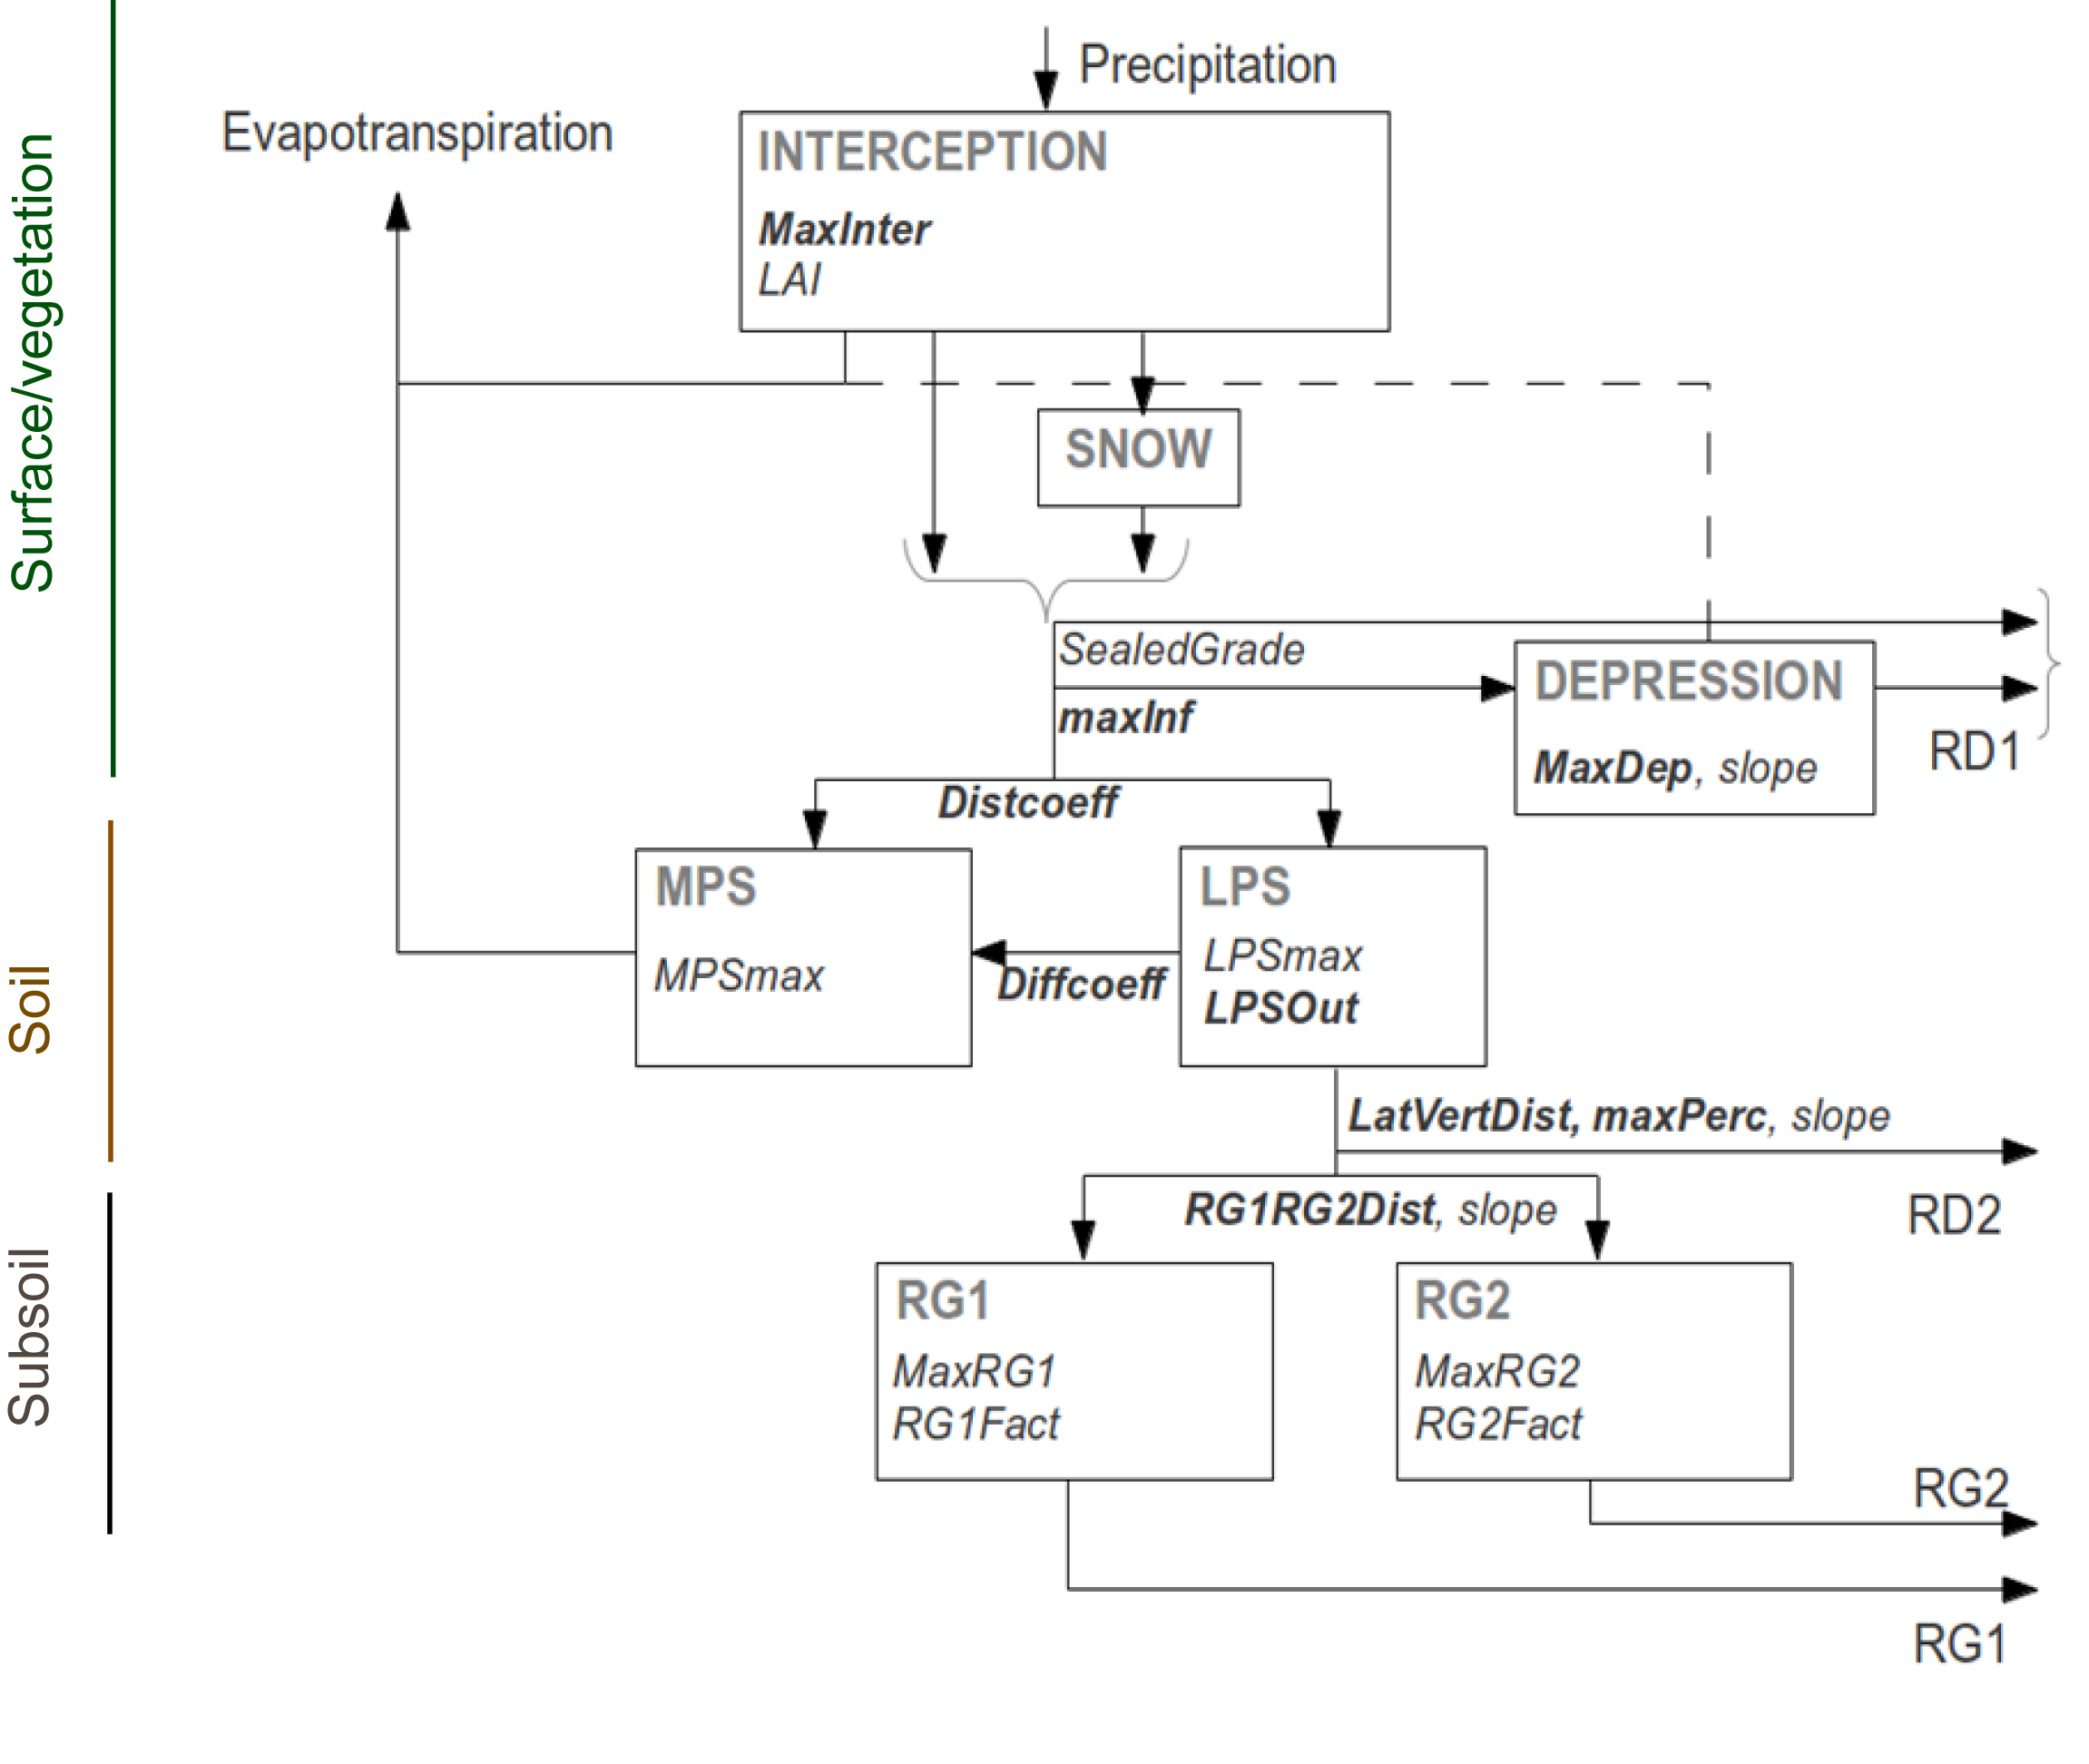
\includegraphics[width=10cm]{Figures/hydro/Figure_2.png}
\caption{Workflow of the J2K hydrological model. \textit{Slightly edited from the J2K documentation.}} 
\label{hydro:fig1}
\end{figure*}

J2K establishes a simulation workflow using temporal (HRU-Loop) and spatial (Time-Loop) contexts, which iterate and perform simulations for each HRU and day of a given catchment and time period. These contexts are implemented in the Jena Adaptable Modelling System (JAMS) platform, in which J2K is integrated. The simulation of specific hydrological processes are performed in components, being separate entities taking a given set of input parameters, processing them and returning multiple output parameters. 

\subsection{An updated glacier module for J2K}

In J2K, the generation of HRUs for a certain catchment can only be done prior to model simulations. The extent and content of HRUs is static in time, preventing the model from making them evolve throughout a simulation. This specificity of J2K makes it difficult for the model to include a dynamic representation of glaciers, explaining why all simulations for glacierized catchments have so far been performed with static glacierized areas \citep{gao_test_2012, nepal_understanding_2014}. In order to overcome this limitation, we have developed an approach allowing the introduction of glacier evolution through time, based on prescribed glacier surface areas. 

A Python package named \textit{Glaciers-to-J2K} has been created, which automatically computes the glacierized fraction of each HRU based on polygons with the extension and surface type of each HRU and annual glacier boundaries. Glacier boundaries can proceed from any glacier model providing annual gridded glacier extents. \textit{Glaciers-to-J2K} computes the glacierized and non-glacierized fraction of each HRU by overlapping HRU outlines with annual glacier extents. Then, these fractions are interpolated with an annual timestep throughout a given ablation season, with a default period between October 1${st}$ to March 31${st}$. This enables a daily representation of glacier area evolution, necessary for hydrological simulations with J2K. These time series are stored in a \textit{.dat} file.

Several components of J2K have been adapted in order to take into account these changes in glacier surface area. 

\subsubsection{Glacier evolution}

Two new components named \textit{GlacierFractionReader} and \textit{GlacierFractionAssigner} have been added, responsible for reading the daily glacierized fractions for each HRU and assigning them to the right HRU during the temporal (Time-Loop) and spatial (HRU-Loop) iterations. 

\subsubsection{Glacier mass balance and runoff}

An already existing glacier module from the J2K model version used in the Himalayas has been updated, creating a new module named \textit{GlacierModuleAlps}. If the glacierized fraction of a given HRU is different than zero, a glacier is detected and the simulation of glacier runoff is triggered. First of all, the snowpack on the glacier is processed with a dedicated snow component, determining the characteristics of snow on the glacier. It simulates accumulation and compaction of the snow pack caused by snow melt or rain. The thermal characteristics under the snow pack are also taken into account with the cold content (CC) of snow (Eq. \ref{hydro:eq:1}).

\begin{equation} \label{hydro:eq:1}
 CC = coldContFact \cdot T
 \end{equation} 
 
where $coldContFact$ is a calibration parameter and T the air temperature at a given HRU. This enables the accumulation of negative temperatures, which are decreased only by positive temperatures, resulting in a potential melting rate. Melting is triggered once the CC has reached zero. Snow occurs when precipitation falls with air temperatures lower than 0ºC. The density of new snow is determined by air temperature follow equation \ref{hydro:eq:3}.

\begin{equation} \label{hydro:eq:2}
 newSnowDens = 0.13 + 0.0135 \cdot T_{acc} + 0.000045 \cdot T_{acc}^{2}
\end{equation} 
 
where $T_{acc}$, which shares the same formulation as the melting temperature ($T_{melt}$), is defined by equation \ref{hydro:eq:3}.

\begin{equation} \label{hydro:eq:3}
 T_{acc} = T_{melt} = \frac{T_{min} + T_{avg}}{2}
\end{equation} 

If air temperature is lower than -15ºC the density of snow is assumed to be 0.02875. At this point, the change in snow depth ($\Delta SH$) from snowfall is determined by equation \ref{hydro:eq:4}.

\begin{equation} \label{hydro:eq:4}
 \Delta SH = \frac{snow}{newSnowDens}
\end{equation} 

Then, the snow water equivalent (SWE) of the previous day ($SWE_{dry}$) is increased with new snow, following equation \ref{hydro:eq:5}.

\begin{equation} \label{hydro:eq:5}
 SWE_{dry,t} = SWE_{dry,t-1} + snow
\end{equation} 

If $T_{melt}$ exceeds a certain threshold value (normally 0ºC) the snow pack transitions from accumulation phase to metamorphosis. The amount of energy available for melt is computed in three different ways: (1) the sensible heat from air temperature ($t_{snow}$), (2) the energy input from rain ($r_{factor}$), and (3) the energy input from soil heat flow ($g_{factor}$). The sum of these three components gives the potential snow melt rate ($M_{p}$), defined by equation \ref{hydro:eq:6}.

\begin{equation} \label{hydro:eq:6}
 M_{p} = (t_{snow} \cdot T_{melt} + r_{factor} \cdot rain \cdot T_{melt} + g_{factor}) \cdot \theta
\end{equation} 

where $\theta$ is a parameter modifying the melt according to the slope and aspect of the HRU. At this point, $M_{p}$ is used to update the $CC$ and the maximum change in the snow pack (Eq. \ref{hydro:eq:7}).

\begin{equation} \label{hydro:eq:7}
 \Delta SH = \frac{M_{p}}{dry_{density}}
\end{equation} 

where $dry_{density}$ is the snow dry density. If $\Delta SH$ is greater than the entire snow depth, it melts completely and the entire SWE contributes to runoff generation. If this is not the case, $SH$ is reduced accordingly, leading to an increase in the total snow density ($tot_{dens}$). Additionally to this change of density, changes in subsidence and density following the snow compaction scheme \citep{bertle_effect_1966} are taken into account. Water seeps into the snow pack, contributing to subsidence by recyrstallization of snow and by structural changes. This subsidence rate is computed using the snow-subsidence method, whose increase of accumulated water content in percentage is determined by equation \ref{hydro:eq:8}.

\begin{equation} \label{hydro:eq:8}
 P_{w} = \frac{SWE_{tot}}{SWE_{dry}}100
\end{equation} 

The greater the liquid water in input, the great the snow pack subsidence will be. The percentage of snow depth change ($P_{H}$) is computed from the input of free water (Eq. \ref{hydro:eq:9}).

\begin{equation} \label{hydro:eq:9}
 P_{H} = 147.4 - 0.474 \cdot P_{w}
\end{equation} 

allowing the calculation of the new snow depth ($SD$).

\begin{equation} \label{hydro:eq:10}
SH = SH\frac{P_{H}}{100}
\end{equation} 

Finally, the dry snow density ($dry_{dens}$) and the total snow density ($tot_{dens}$) are recomputed taking into account this updated snow depth (Eqs. \ref{hydro:eq:11} and \ref{hydro:eq:12}). 

\begin{equation} \label{hydro:eq:11}
dry_{dens} = \frac{SWE_{dry}}{SD}
\end{equation} 

\begin{equation} \label{hydro:eq:12}
tot_{dens} = \frac{SWE_{tot}}{SD}
\end{equation} 

The snow pack can store liquid water in its pores up to a certain critical density ($snow_{critDens}$). When a certain amount of liquid water is reached with respect to the total SWE (about 40-45\%), this storage is released \citep{bertle_effect_1966}. This process is taken into account in the model by computing a maximum water content in the snow pack ($SWE_{max}$), following equation \ref{hydro:eq:13}.

\begin{equation} \label{hydro:eq:13}
SWE_{max} = snow_{critDens}\cdotSD
\end{equation} 

The $snow_{critDens}$ needs to be provided by the user. Finally, the snow runoff ($Q_{snow}$) is determined by the water stored in the snow pack that exceeds this limit (Eq.\ref{hydro:eq:14}).

\begin{equation} \label{hydro:eq:14}
Q_{snow} = SWE_{tot} - SWE_{max}
\end{equation} 

Through time (daily time steps in our case), the snow pack can keep this critical threshold density until being defrosted or new snowfall occurs. 

If no snow is present in a given glacierized HRU, ice melt can occur. This is computed using a temperature-index melt model \citep{hock_temperature_2003}, following equation \ref{hydro:eq:15}.

\begin{equation} \label{hydro:eq:15}
ice_{melt} = \frac{1}{n}t_{ice} + \alpha_{ice } \cdot Q_{radiation} \cdot(T_{melt} - T_{base})
\end{equation} 

where $n$ is the time stemp ($n$ = 1 for a daily model), $t_{ice}$ is a melt factor specific for ice, $\alpha_{ice}$ is a fixed ice melt coefficient based on albedo, $Q_{radiation}$ is the actual global solar radiation and $T_{base}$ is a based temperature defined by the user to trigger melt (normally 0ºC). The previously existing glacier module implemented in the Himalayas also takes into account the effects of debris cover, which will not be described here since they have not been implemented in this work due to time constraints. 

Finally, snow melt and ice melt are further adapted depending on the slope and aspect of each HRU (Eqs. \ref{hydro:eq:16} and \ref{hydro:eq:17}).

\begin{equation} \label{hydro:eq:16}
Q_{snow} = (r_{t-1 }\cdot e^{(1/k_{snow})} \cdot Q_{snow} \cdot e^{(1/k_{snow})})g_{fraction}
\end{equation} 

\begin{equation} \label{hydro:eq:17}
Q_{ice} = (r_{t-1} \cdot e^{(1/k_{ice})} \cdot Q_{ice} \cdot e^{(1/k_{snow})})g_{fraction}
\end{equation} 

where $r_{t-1}$ is the outflow reservoir during the previous time step; $k_{snow}$ and $k_{ice}$ are storage coefficients for the reservoirs, determined by the user; and $g_{fraction}$ is the glacierized fraction of the HRU, used to scale the runoff coming from glaciers. 

\subsubsection{Non-glacierized fraction}

Glacierized HRUs might contain a non-glacierized fraction as well. The runoff computed outside the glacier, within the previously existing workflow in J2K, is multiplied by the non-glacierized HRU fraction ($1/g_{fraction}$). This enables an accurate separation between glacierized and non-glacierized runoff contributions for each HRU. 

\subsubsection{Mass balance calibration}

Therefore, this new glacier module computes glacier mass balance with a daily timestep. In order to correctly calibrate glacier mass balance, three parameters can be tuned: a precipitation lapse rate specific for the glacier, a snow melt factor ($t_{snow}$) and an ice melt factor ($t_{ice}$). Precipitation is known to be underestimated in climate datasets in the French Alps, for both the SAFRAN and SPAZM datasets used in this PhD work \citep{vionnet_numerical_2016}. This means that increasing precipitation via a lapse rate factor is often needed in order to correctly reproduce accumulation rates on glaciers. 

This implemented approach can be easily escalated to glacierized catchments with multiple glaciers. Every HRU has an ID which can be matched to any Randolph Glacier Inventory (RGI) ID, allowing a specific calibration of mass balance models for each individual glacier. In catchments with small glaciers located close together, these might end up sharing an HRU. For these cases, the optimization of the melt model would have to be shared among all the glaciers present in that HRU. Alternatively, the size of the HRU separation can be reduced, improving the spatial representation of the catchment. Nonetheless, this has an important computational cost. We believe this updated modelling framework has enough flexibility to enable an accurate calibration of different melt factors and precipitation lapse rates in mountainous regions. 

\section{Results}

This updated glacier module for the J2K hydrological model has been implemented and validated in the Arvan semi-glacierized catchment in the French Alps.

\subsection{Glacer evolution}

\subsection{Glacier mass balance}

In order to calibrate the temperature-index model in J2K, we used seasonal (winter and summer) glacier-wide MB data from the GLACIOCLIM glacier observatory on the Saint Sorlin glacier. The precipitation lapse rate was calibrated based on winter mass balance data, and the ice and snow melt factors on summer mass balance data. Due to time constraints, this calibration was performed manually. J2K includes a parameter optimization module, but the recalculation of glacier mass balance from a daily to seasonal frequency was performed outside J2K, in the Glaciers-to-J2K Python package, in order to accelerate the development. In the future, this recalculation should be moved inside J2K to enable the automatic calibration of the precipitation lapse rate and melt factors for ice and snow for large catchments. 

\subsection{Glacier runoff}

\section{Discussion and conclusions}

\section{Code availability}

The source code of the Python package \textit{Glaciers-to-J2K} is available in the following GitHub repository: https://github.com/JordiBolibar/Glaciers-to-J2K

\section{Appendix}

\begin{sidewaysfigure}[h]
\centering
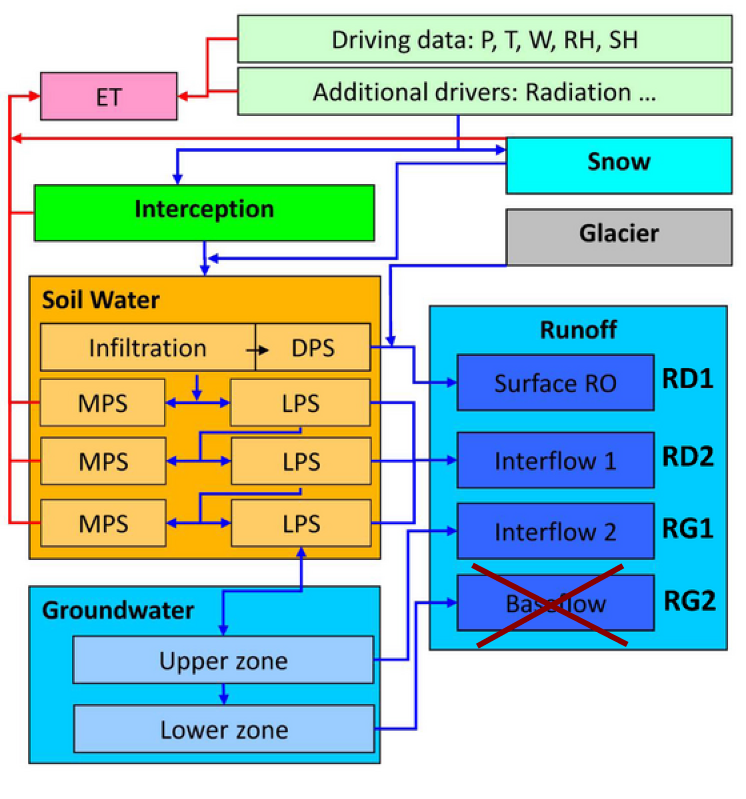
\includegraphics[width=23cm]{Figures/hydro/Figure_1.png}
\captionsetup{justification=centering}
\caption{Description of the Arvan catchment, based on hydrological data observed at the Saint-Jean-d'Arves (La Vilette) station. 
\textit{Figure from the HYDRO team from INRAE Antony}.}
\label{hydro:figA1}
\end{sidewaysfigure}






\part{Outlook}

\chapter{Conclusions and perspectives}
\label{chap:discussion}

\begin{flushright}
\begin{small}
\textit{In the study of nature, as in the practice of art, it is not given to man to achieve the goal without leaving a trail of dead ends he had pursued.}\\ \\
Baron Louis Bernard Guyton de Morveau
\end{small}
\end{flushright}

\section{Summary of the results}

The initial objective of this PhD work was to study the evolution of all glaciers in the French Alps from the last decades of the 20$^{th}$ century until the end of the 21$^{st}$ century, and to explore the impact of their retreat in the hydrological budget of the Rhône river catchment. However, this initial objective was adapted following the exploration of machine learning methods for glacier mass balance simulation at the end of the first year of the project. My strong interest in these rather unexploited methods in glaciology lead to important changes in the results, largely expanding the efforts dedicated on methods, and reducing the amount of results on hydroglaciological modelling. Consequently, the resulting scientific questions that were addressed during these three years also evolved. In this section, I will address each one of these questions, giving an overview of the results and determining the accomplished objectives as well as the remaining challenges.

\subsubsection{Question 1 - Can deep learning be applied to model annual glacier mass balance changes at a regional scale? What are the benefits of using nonlinear deep learning models compared to linear machine learning?}

In Chapter 2, based on a paper published in \textit{The Cryosphere} journal, we introduced, to our knowledge, the first effort ever to apply deep learning to simulate glacier evolution. A new open-source regional glacier evolution model was developed, whose main novelty was a mass balance component based on machine learning. Our work showed promising results, proving that deep learning can be successfully used to simulate glacier mass balance. A detailed comparison between linear machine learning methods and deep learning highlighted how important nonlinearities are captured by deep learning. Since both the climate and glacier systems are known to be highly nonlinear, this resulted in an improved performance from deep learning models. Moreover, despite using a rather small dataset of annual mass balance data, we proved that by rigorously cross-validating the models, deep learning can still learn from "small data" without overfitting. Spatiotemporal data demands that the independence of both dimensions have to be respected during cross-validation. We devised different types of cross-validation which enabled us to accurately evaluate the performance of models in the spatial and temporal dimensions, while fully utilizing the whole dataset to train the models. 

\subsubsection{Question 2 - What are the annual glacier changes of all glaciers in the French Alps for the last half century?}

In Chapter 3, based on a paper published in the \textit{Earth System Science Data} journal, we applied the deep learning methods developed in Chapter 2 to the reconstruction of annual glacier-wide MB series of all glaciers in the French Alps between 1967 and 2015. Our results showed that French alpine glaciers went through slightly negative MB rates from the late 1960s and during the 1970s (-0.44 m.w.e. a$^{-1}$). Then, during the 1980s  their MB was almost stable (-0.16 m.w.e. a$^{-1}$, with several positive years), before becoming more negative from the 1990s (-0.71 m.w.e. a$^{-1}$). Their MB rates became remarkably more negative from the 2000s (-1.18 m.w.e. a$^{-1}$), especially after the famous heatwave from the year 2003. This year established an inflection point, from which MB became increasingly negative up to -1.26 m.w.e. a$^{-1}$ for the first half of the 2010s. Important differences were found between massifs, with the Mont-Blanc massif showing the least negative MB, and the Chablais massif presenting the highest losses. We showed how this method correctly captured the interannual variability of the glacier-wide MB signal of glaciers in the French Alps, mostly driven by climate, and how it also captured differences between glaciers with various topographical characteristics. 

\subsubsection{Question 3 - How will French alpine glaciers evolve during the 21st century? How does glacier retreat affect the climate signal on glaciers? What are the main factors that determine glacier survival in the French Alps?}

\blindtext

\subsubsection{Question 4 - What are the current limitations in the representation of glaciers in hydrological models in France? How can we improve this?}

Current hydrological models in France generally suffer from a simplified representation of glaciers as static ice reservoirs. This is highly problematic in the current context of rapid glacier retreat in the French Alps. Glacio-hydrological models need to accurately represent glacier evolution in order to take into account the progressive changes in hydrologic regime, seasonality and glacier runoff. These changes can drive important social and environmental impacts in the French Alps, which demand adequate tools to perform accurate glacio-hydrological projections. In this work, we introduced an updated glacier module for the well-established J2K hydrological model \citep{krause_quantifying_2002}, capable of representing the daily evolution of glaciers. This approach is based on prescribed annual glacier extents, that can proceed from any glacier evolution model. We validated this method in the Arvan partially glacierized catchment, located in the Grandes Rousses massif, for which we also assessed the effects of glacier retreat on the recent past. With this new enhanced representation of glaciers in the J2K hydrological model, we have set the means for future glacio-hydrological studies in the Rhône river catchment to assess the hydro-ecological impacts of glacier retreat. 

\section{Perspectives on future research venues}

This PhD work served to bring attention to the benefits of using deep learning for regression problems in glacier evolution modelling. At the beginning of this PhD, to my knowledge, there were no papers published using deep learning on glaciers. For the AGU Fall Meeting 2019, a new session on machine learning, artificial intelligence (AI) and remote sensing on the cryosphere was created for the first time. This session served to catalyse all the current research in this sub-field, with many papers published around that period. For the first time, researchers working on these topics were able to exchange, discuss and even collaborate in bringing new methods to different applications in glaciology. This experience was followed by another session on machine learning and AI for glaciology at the EGU General Meeting 2020, which despite the virtual format due to the global COVID-19 crisis, further displayed the huge potential of these applications from a wide range of glaciological problems. Machine learning and data science in glaciology is still a very novel field, but many promising applications are being presented by the day \citep[e.g.][]{leong_deepbedmap_2020, brinkerhoff_constraining_2020}, showing multiple directions for the sub-field to evolve towards. 

So far, as it was shown in these two previous sessions at AGU and EGU, the great majority of efforts have been focused on classification problems. New satellite imagery, with ever improving spatial and temporal resolution, is being successfully exploited by deep learning methods to automatically extract glacier fronts in Greenland and Antarctica \citep[e.g.][]{lea_google_2018,baumhoer_automated_2019,mohajerani_detection_2019, zhang_automatically_2019} and supraglacial lakes \cite[e.g.][]{yuan_automatic_2020}. The validation of this approaches is more straightforward than for regression problems, mainly demanding the manual delineation or classification of geometric features in satellite imagery. Moreover, in such applications where interpretability is not a concern, the full predictive power of convolutional NNs can be unleashed. Conversely, regression problems in glaciology remain highly unexplored, due to the inherent complexity of correctly representing physical processes with NNs. This brings us to the last scientific question of this PhD work.

\subsubsection{Question 5 - What are the caveats of the deep learning modelling approach used in this work? What improvements are needed to overcome these limitations for glaciological studies?}

The work of this PhD showed how deep learning models can be extremely challenging to interpret. We attempted to partially do so by training a parallel linear machine learning model (Lasso) with the same dataset, and by thoroughly cross-validating it respecting spatiotemporal structures in data. Nonetheless, these represented just approximations of what the true underlying model actually is, and raised many questions on how to address these issues. 

Fortunately, in the last years enormous progress has been made towards interpretable machine learning and particularly interpretable NNs. NNs are universal function approximators, meaning that any sufficiently large NN can approximate any nonlinear function with a finite set of parameters \citep{winkler_performance_2017}. This remarkable predicting power comes at the cost of very low interpretability, requiring deep changes in the way we design NNs. In order to represent a partially known physical process with a NN, two main approaches are being proposed nowadays: (1) NNs are optimized following a certain loss function, which determines how they learn and update the weights of the different connections between neurons. By consciously modifying a NN's architecture, one can constrain the way NNs learn based on prior knowledge. The most prominent way so far has been to encode prior knowledge, in the form of differential equations (DEs), as the loss function of a NN. By doing so, the learning of NNs is constrained following currently known equations \citep{raissi_physics_2017,karpatne_physics-guided_2018}. Additionally, by using specific architectures that suit the specificities of a given physical process, the learning can be further constrained, limiting or enhancing the interactions between certain input predictors \citep{karpatne_theory-guided_2017}. Such an approach enables an equation-guided learning, but does not fully deal with the "black box" consequences on interpretability. (2) Another way of looking at this problem is that, instead of trying to constrain the learning of NNs, NNs can be reduced to the smallest possible entities, in order to decrease their complexity to the point they can be interpreted. This radically different approach is currently showing very exciting results. The beauty of this approach resides on the fact that it manages to create hybrid models, mixing a classical physical approach based on DEs with the phenomenal predictive power of NNs to optimize unknown parameters \citep{rackauckas_universal_2020}. The main structure of such a model remains a DE, which is augmented with NNs that replace the unknowns parameters. New methods enable the optimization of DEs combined with NNs, allowing the NNs to produce nonlinear functions that optimize the unknowns following an equation determined by the DE \citep{raissi_physics_2017,rackauckas_universal_2020,bradbury_jax_2020}. Since these "small" NNs are based on just one or two input predictors, their output values can be sampled using Monte Carlo methods at their input. By applying a sparse regression on its outputs, one can obtain a mathematical representation of the nonlinear function learnt by the NN \citep{brunton_discovering_2016}. This mathematical representation of NNs can be used to interpret them, while suggesting reformulations in the currently known equations used in the model \citep{rackauckas_universal_2020}. 

The sub-field of glacier machine learning and data science is ripe for progress, and many innovative studies are offering new perspectives on how to improve our understanding of glacier processes with models. Not all solutions go through NNs, as a study by \citet{werder_bayesian_2019} recently showed. They applied a Bayesian inference inverse model to estimate glacier ice thickness. By reusing an already established model describing the ice thickness distribution of glaciers, they were able to assimilate observations for the optimization of model parameters with a detailed assessment of their uncertainties and errors. \citet{rounce_quantifying_2020} followed a similar approach on regional modelling of glacier MB, providing new insight on the main sources of model uncertainty. More recently, a study by \citet{brinkerhoff_constraining_2020} took this approach to another level by applying it to a surrogate model based on deep learning. Bayesian inference can be computationally expensive, and its application to highly complex models involving several parameters, such as a 3D spatially-explicit hydrological model coupled with ice dynamics, is not feasible for now. In this study, they bypassed this limitation by substituting this model with a "black box" NN, producing an equivalent solution at a fraction of the computational cost. This surrogate model allowed the use of Bayesian inference in order to correctly estimate parameter uncertainties and errors. Such diverse approaches display new ways of tackling glaciological modelling, that can provide major changes in our understanding of glacier processes. 

These new methods offer a great perspective to overcome the main limitations of our current glacier evolution modelling approach. By reusing currently known equations of glacier processes, such as the Shallow Ice Approximation \citep{hutter_theoretical_1983} or enhanced temperature-index or surface energy balance models, we can aim at building new methods on top of the most reliable theoretical bases in our field. This offers the possibility to optimize and potentially reformulating these equations, in order to exploit data using NNs in an interpretable manner, creating knowledge that can be reused by the whole glaciological community. During the last year of my PhD, I have been thinking about and developing these ideas, gathering them in the form of a postdoc proposal. With it, I propose to use hybrid models composed by differential equations and NNs to simulate glacier evolution at a large scale. Such an approach can potentially enable a detailed interpretation of specific glacier processes (e.g. ice dynamics) from parameters optimized by NNs, which could be taken into account by reformulating currently known equations. I hope to be able to continue investigating this line of research, as I keep learning from these two fascinating research fields that are glaciology and machine learning. 



%\includepdf[scale=0.9,frame=true,pages=-,pagecommand={\thispagestyle{fancy}}]{D:/01_these/manuscrit/latex_files/list_publications/Brun_et_al_2016_JoG_ice-cliffs.pdf}

%\begin{small}
%\input{list_acronyms/list_acronyms}
%
%
%\listoffigures
%\addcontentsline{toc}{chapter}{List of figures} 
%\listoftables
%\addcontentsline{toc}{chapter}{List of tables} 
%\end{small}
%
%\newpage
%\input{publications.tex}
%\newpage


\linespread{1.}
\begin{small}

\bibliographystyle{copernicus}


\bibliography{references}
\addcontentsline{toc}{chapter}{Bibliography} 

\end{small}


\end{document}
%\addcontentsline{toc}{part}{Conclusion}















